\documentclass[UTF8, heading=true]{ctexart}
\usepackage{karnaugh-map}
%-----中文宏包-----
\usepackage{ctex}
\usepackage[UTF8]{ctex}
\usepackage{titling}
%-----数学宏包-----
\usepackage{amsmath,amsthm,amssymb,amsfonts}
\usepackage{mathrsfs,bm}
\usepackage{dirtree}
%-----draft下 label提示-----
%\usepackage[notcite,notref]{showkeys}
%-----页面布局-----
\usepackage{geometry}
\usepackage{stmaryrd}
\geometry{left=1.25in,right=1.25in,top=1in,bottom=1in}
%\geometry{left=1in,right=1in,top=1in,bottom=1in}
%\geometry{left=2.5cm,right=2.1cm,top=1.7cm,bottom=2cm,includehead,includefoot}

%-----设置超链接-----
\usepackage{url,hyperref}
\hypersetup{colorlinks=true,linkcolor=black,citecolor=black} % 去掉目录红框
%-----制作目录-----
\usepackage{imakeidx}
% 设置颜色
% \usepackage{color,xcolor}
% 插入图片
\usepackage{graphicx}
\usepackage{epsfig}
%-----设置表格-----
\usepackage{tabularx,array}
\usepackage{longtable}
\usepackage{booktabs}
\usepackage{multirow}
\usepackage{multicol}
\usepackage{fancybox}
%-----调整单元格格式-----
\usepackage{makecell}
%-----操作字符串-----
\usepackage{xstring}
%-----多语种处理-----
%\usepackage[english]{babel}
%-----设置代码环境-----
\usepackage{listings}
%-----设置章节标题和目录-----
\usepackage{titletoc}
\usepackage{titlesec}
%-----数学公式扩展-----
\usepackage{mathtools}
%-----浮动体设置-----
\usepackage{float}
%-----书签设置-----
\usepackage{bookmark}
%-----参考文献格式-----
\usepackage[numbers]{natbib}
%-----设置页眉页脚格式-----
\usepackage{fancyhdr}
\usepackage{minted}
\definecolor{bg}{rgb}{0.95, 0.95, 0.95}

\usepackage{algorithm}
\usepackage{algpseudocode}
\usepackage{setspace}
\floatname{algorithm}{Algorithm}
\algrenewcommand\algorithmicrequire{\textbf{输入:}}
\algrenewcommand\algorithmicensure{\textbf{输出:}}


% 设置 minted 环境的全局选项
\setminted{
    linenos, % 显示行号
    frame=lines, % 添加边框
    framesep=2mm, % 设置边框与代码之间的间距
    breaklines, % 自动换行
    bgcolor=bg, % 设置背景颜色
    baselinestretch = 1.0,
    numbersep = 5pt,
    numberblanklines = false,
	tabsize = 4
}

\geometry{
  left=3.0cm,        % 左边距
  right=3.0cm,       % 右边距
  top=2.5cm,         % 上边距
  bottom=2.0cm       % 下边距
}
\renewcommand*{\baselinestretch}{1.5}
\newcommand{\upcite}[1]{\textsuperscript{\textsuperscript{\cite{#1}}}}

\renewcommand{\thesection}{\chinese{section}、}
\renewcommand{\thesubsection}{(\chinese{subsection})}
\renewcommand{\thesubsubsection}{\arabic{subsubsection}.}
\titleformat{\section}{\bfseries \zihao{-3}}{\chinese{section}、}{0em}{}
\titleformat{\subsection}{\bfseries \zihao{4}}{(\chinese{subsection})}{0.2em}{}
\titleformat{\subsubsection}{\bfseries \zihao{-4}}{\arabic{subsubsection}. }{0.2em}{}
\newcommand{\stunum}[1]{\def\defstunum{#1}}
\newcommand{\class}[1]{\def\defclass{#1}}

% ----- 设置浮动体间距 ------
\setlength{\textfloatsep}{0pt}
\setlength{\floatsep}{10pt plus 3pt minus 2pt}
\setlength{\intextsep}{10pt}
\setlength{\abovecaptionskip}{2pt plus1pt minus1pt}
\setlength{\belowcaptionskip}{3pt plus1pt minus2pt}

% ----- 设置公式间距为零 ------
\AtBeginDocument{
	\setlength{\abovedisplayskip}{4pt plus1pt minus1pt}
	\setlength{\belowdisplayskip}{4pt plus1pt minus1pt}
	\setlength{\abovedisplayshortskip}{2pt}
	\setlength{\belowdisplayshortskip}{2pt}
	\setlength{\arraycolsep}{2pt}   % array中列之间空白长度
}

% ---- 定义列表项的样式 -----
\usepackage{enumitem}
\setlist{nolistsep}
% \setlength{\itemsep}{3pt plus1pt minus2pt}

% --- 设置英文字体 -----
% \usepackage{newtxtext}  % for text fonts
\usepackage{fontspec}
\setmainfont{Times New Roman}
% --- 设置数学字体 -----
% \usepackage{newtxmath}
% \usepackage{mathptmx}



% --- 设置代码环境 -----
\usepackage{listings}
\usepackage{color,xcolor}

% --- 自定义命令 -----
\newcommand{\CC}{\ensuremath{\mathbb{C}}}
\newcommand{\RR}{\ensuremath{\mathbb{R}}}
\newcommand{\A}{\mathcal{A}}
\newcommand{\ii}{\bm{\mathrm{i}}\,}  % 虚部
\newcommand{\md}{\mathrm{d}\,}
\newcommand{\bA}{\boldsymbol{A}}
\newcommand{\red}[1]{\textcolor{red}{#1}}

\pagestyle{fancy}
\fancyhf{}
\fancyfoot[C]{\thepage}
\fancyhead[L]{离散数学章节自测题汇总}
\fancyhead[R]{Tony 计算机科学与技术}
\title{\LARGE \textbf{离散数学章节自测题汇总}}
\author{Tony \hspace{2.89cm} 计算机科学与技术}
\begin{document}
\maketitle

\thispagestyle{fancy}
% -----------------从这里开始写文章-----------------

\textbf{写在前面:}这篇文档结合了多位同学的学习通题目,旨在方便大家复习离散数学,\textbf{仅供学习交流使用},如有侵权,请联系删除。
\textbf{不要只看题目序号,选项可能会换顺序!!!}由于题目数量大,文档中难免会有小的文字识别错误,还望谅解。


\phantomsection
\addcontentsline{toc}{section}{前言}
\section*{前言}

\subsubsection{测验题0.1}

下面说法正确的有:

A. 离散数学是以可枚举的数量或形状作为研究对象的数学分支。

B. 离散数学中可枚举的含义是指研究对象与若干自然数有一一对应关系。

C. 学习离散数学课程知识必须具有一定的编程能力。

D. 学习离散数学课程可以对逻辑,集合,排列组合等相关基础知识完全没有了解。

E. 课程所用教材《离散数学基础》正文中与"例子"一起编号的"问题"需要学生自己解答。

\textcolor{red}{答案:ABD}

\subsubsection{测验题0.2}

离散数学基础课程应该学习的离散数学语言包括:

A. 逻辑语言

B. 集合语言

C. 算法语言

D. 图论语言

E. 代数语言

\textcolor{red}{答案:ABCDE}

\subsubsection{测验题0.3}

计算机类专业的离散数学基础课程应该培养的专业思维包括:

A. 逻辑思维

B. 关系思维

C. 量化思维

D. 计算思维

E. 递归思维

\textcolor{red}{答案:ABCDE}

\subsubsection{测验题0.4}

计算机类专业的离散数学基础课程应该培养的专业意识包括:

A. 离散化

B. 模块化

C. 层次化

D. 系统化

E. 公理化

\textcolor{red}{答案:ABCDE}

\clearpage

\section{基础知识}

\subsubsection{测验题1.1}

下面命题真值为真的命题是?

A. 2020年是闰年而且2021年是闰年。

B. 2021年是闰年或者2022年是闰年。

C. 如果2021年是闰年, 则2022年是闰年。

D. 2020年是闰年当且仅当2021年是闰年。

\textcolor{red}{答案:C}

\textcolor{red}{解析:C中前件为假,蕴涵式为真。}

\subsubsection{测验题1.2}
下面表达“年份是4的倍数”是“年份是闰年”的必要条件的句子是?

A. 一个年份是 4 的倍数时, 则它是闰年。

B. 只有一个年份是4的倍数时, 它才是闰年。

C. 只要一个年份是 4 的倍数, 则它是闰年。

D. 一个年份是4的倍数, 仅当它是闰年。

\textcolor{red}{答案:B}

\subsubsection{测验题1.3}

下面句子中是全称量化命题的是?

A. 有的年份不是 4 的倍数, 但它是闰年。

B. 1900年是4的倍数,但它不是闰年。

C. 如果2020年是闰年, 则有的闰年年份不是 100 的倍数。

D. 一个年份是闰年当且仅当它是 4 的倍数。

\textcolor{red}{答案:D}

\subsubsection{测验题1.4}

\textit{出自Raymond Smullyan的``Logic Labyrinths''}

人类学家Edgar Abercrombie来到一个岛上,这个岛上的居民要么是骑士(Knight),要么是无赖(Knave),二者必居其一,骑士总是说真话,而无赖总是说假话。Abercrombie碰到了岛上三个居民A, B, C。他问A:“你是骑士还是无赖?”A回答了,但是Abercrombie没有听清,于是他问B:“刚才A说什么?”,B回答说:“A说他是无赖。”这时C大声说:“不要相信B,他说谎!”根据这个故事,下面正确的是?

A. 可以断定A是骑士

B. 可以断定A是无赖

C. 可以断定 B 是骑士

D. 可以断定C是骑士

\textcolor{red}{答案:D}

\textcolor{red}{解析:假如A是无赖,那么A只会说自己是骑士;如果A是骑士,那么A会说自己是骑士。不管A如何,B说的都一定是假话,即B是无赖。
也就可以推出C说的是真话,即C是骑士。A到底是什么无法判断。}

\subsubsection{测验题1.5}

设 $P=\left\{x \in \mathbb{Z}^{+} \mid x\right.$ 是质数且小于 10$\}, Q=\left\{x \in \mathbb{Z}^{+} \mid x\right.$ 是大于 1 且小于 9 的奇数 $\}$,
下面正确的是?

A. $P \in Q$

B. $P \subseteq Q$

C. $Q \in P$

D. $Q \subseteq P$

\textcolor{red}{答案:D}

\subsubsection{测验题1.6}

设 $D=\{1,2,3,4\}, Q=D \times D$, 在 $Q$ 上定义关系 $R$, 对任意 $a, b, c, d \in D,\langle a, b)$ 和 $\langle c, d\rangle$ 有关系 $R$, 当且仅当 $a \cdot d=b \cdot c$ (这里•是整数乘法), 即:
$$
\langle\langle a, b\rangle,\langle c, d\rangle\rangle \in R \text { 当且仅当 } a \cdot d=b \cdot c
$$

下面属于 $R$ 的元素是?

A. $<1,2>$

B. $<<1,2>,<2,4>>$

C. $<<1,2>,<4,2>>$

D. $<<1,3>,<2,6>>$

\textcolor{red}{答案:B}

\subsubsection{测验题1.7}

归纳定义集合 $A$ :

(1) \textcolor{blue}{\textbf{归纳基}}: $4 \in A$ 且 $6 \in A$;

(2) \textcolor{blue}{\textbf{归纳步}}: 如果 $a \in A$ 和 $b \in A$, 则 $a+b \in A$, 这里$+$是整数加法。下面不属于集合 $A$ 的元素是?

A. 20

B. 21

C. 22

D. 26

\textcolor{red}{答案:B}

\subsubsection{测验题1.8}

下面在定义函数时错误的是?

A. 定义函数 $f: \mathbb{N} \rightarrow \mathbb{N}, \forall x \in \mathbb{N}, f(x)=x+1$ 。

B. 定义函数 $f: \mathbb{R} \rightarrow \mathbb{R}, \forall x \in \mathbb{R}$, 如果 $x$ 是有理数, 则 $f(x)=1$, 否则 $f(x)=-1$ 。

C. 定义函数 $f: \mathbb{R} \rightarrow \mathbb{R}, \forall x \in \mathbb{R}, f(x)=\sqrt{2 x+1}$ 。

D. 定义函数 $f:\{1,2,3,4\} \rightarrow\{1,2,3\}, f(1)=f(2)=f(3)=1, f(4)=2$ 。

\textcolor{red}{答案:C}

\subsubsection{测验题1.9}

下面哪个选项给出的不是连通图?

\begin{figure}[htbp]
    \centering
    \begin{minipage}[t]{0.35\textwidth}
        \centering
        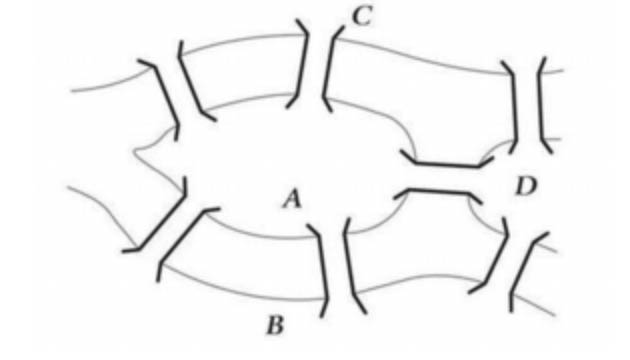
\includegraphics[width=1\textwidth]{1.9_1.jpg} % 插入图片
        \caption{测验题1.9 A选项}
    \end{minipage}
    \hfill
	%   \hspace{0.1\textwidth} % 调整这里的值来改变两张图片之间的间距
    \begin{minipage}[t]{0.35\textwidth}
        \centering
        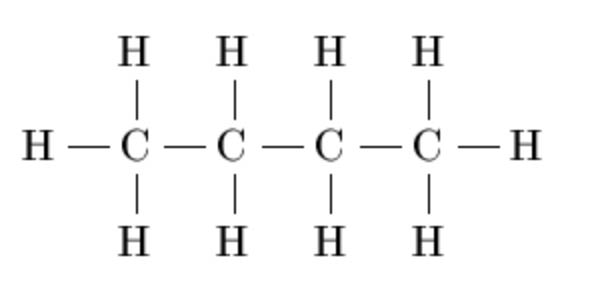
\includegraphics[width=1\textwidth]{1.9_2.jpg} % 插入图片
        \caption{测验题1.9 B选项}
\end{minipage}
\end{figure}

\begin{figure}[htbp]
  \centering
  \begin{minipage}[t]{0.35\textwidth}
      \centering
      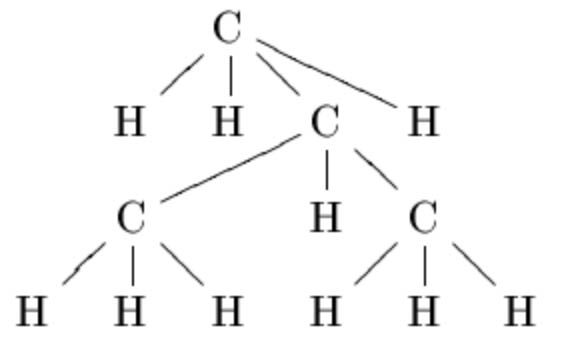
\includegraphics[width=1\textwidth]{1.9_3.jpg} % 插入图片
      \caption{测验题1.9 C选项}
  \end{minipage}
  \hfill
%   \hspace{0.1\textwidth} % 调整这里的值来改变两张图片之间的间距
  \begin{minipage}[t]{0.35\textwidth}
      \centering
      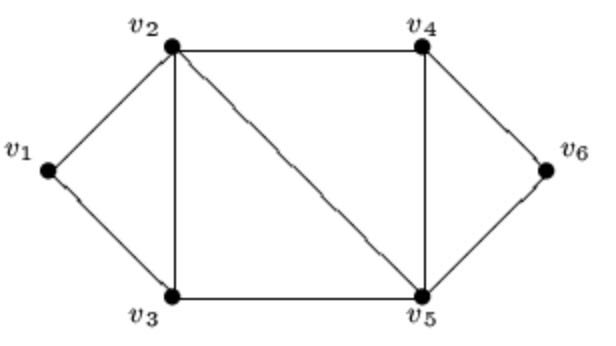
\includegraphics[width=1\textwidth]{1.9_4.jpg} % 插入图片
      \caption{测验题1.9 D选项}
\end{minipage}
\end{figure}

\textcolor{red}{答案:A}

\textcolor{red}{解析:???}

\subsubsection{测验题1.10}

下面哪个选项给出的是无向树?

\begin{figure}[htbp]
  \centering
  \begin{minipage}[t]{0.2\textwidth}
      \centering
      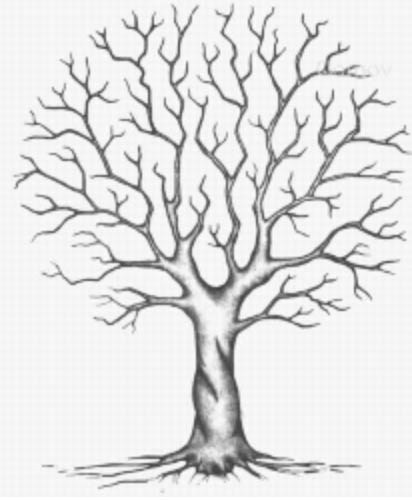
\includegraphics[width=1\textwidth]{1.10_1.jpg} % 插入图片
      \caption{测验题1.10 A选项}
  \end{minipage}
  % \hfill
  \hspace{0.1\textwidth} % 调整这里的值来改变两张图片之间的间距
  \begin{minipage}[t]{0.35\textwidth}
      \centering
      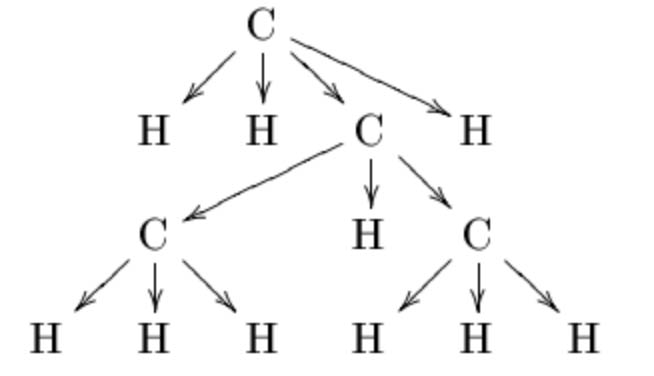
\includegraphics[width=1\textwidth]{1.10_2.jpg} % 插入图片
      \caption{测验题1.10 B选项}
\end{minipage}
\end{figure}

\begin{figure}[htbp]
\centering
\begin{minipage}[t]{0.35\textwidth}
    \centering
    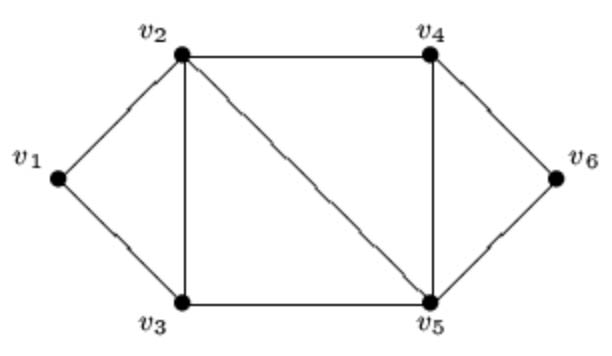
\includegraphics[width=1\textwidth]{1.10_3.jpg} % 插入图片
    \caption{测验题1.10 C选项}
\end{minipage}
% \hfill
  \hspace{0.1\textwidth} % 调整这里的值来改变两张图片之间的间距
\begin{minipage}[t]{0.35\textwidth}
    \centering
    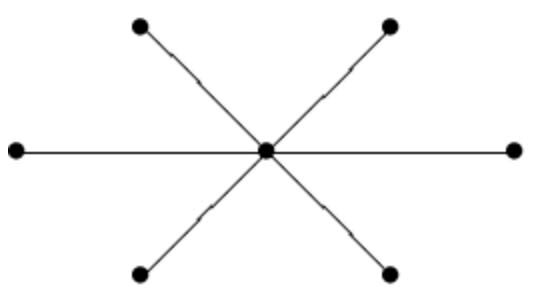
\includegraphics[width=1\textwidth]{1.10_4.jpg} % 插入图片
    \caption{测验题1.10 D选项}
\end{minipage}
\end{figure}

\textcolor{red}{答案:D}



\subsubsection{测验题1.11}

下面哪个说法是正确的?

A. 开平方根是实数集合上的运算。

B. 减法是自然数集上的运算。

C. 除法是实数集上的运算。

D. 平方是自然数集上的运算。

\textcolor{red}{答案:D}

\subsubsection{测验题1.12}

在实数集R上定义二元运算*:对任意实数x, y,x * y = xy - x - y。下面哪个说法是错误的?

A. 该运算满足交换律。

B. 该运算满足结合律。

C. 该运算没有单位元。

D. 该运算没有零元。

\textcolor{red}{答案:B}

\subsubsection{测验题1.13}

下面哪个说法是不正确的?

A. 算法就是求解一个问题的过程。

B. 算法的步骤必须精确定义,而且每个步骤都可在有限时间内执行完毕。

C. 算法的总执行步骤数必须是有限的, 即经过有限步执行必须终止并产生输出。

D. 算法必须具有通用性, 可用于解决一类问题而不仅仅是某一个具体问题。

\textcolor{red}{答案:A}

\subsubsection{测验题1.14}

下面哪个说法是不正确的?

A. 算法的基本步骤需要对算法要求解的问题进行分析而提炼出来。

B. 算法步骤描述中将基本步骤组合成的复合步骤主要有顺序结构、选择结构和循环结构三种。

C. 递归算法可以既没有选择结构也没有循环结构。

D. 设计算法时不仅要考虑算法的正确性还要考虑算法的效率。

\textcolor{red}{答案:C}

\subsubsection{测验题1.15}

对于算法1.4给出的递归算法:

\begin{algorithm}
    \caption{\textbf{判断一个二进制传是否属于例子1.9定义的集合}}
    \begin{algorithmic}[1]
        \Require 二进制串$u$
        \Ensure \textit{如果$u$属于H返回“是”,否则返回“否”}
        \If{\textit{$u$是串0或串1}}
        \State \Return “是”
        \EndIf
        \If{\textit{$u$具有1v1或0v0的形式}}
        \State \textit{返回以v为输入执行本算法的结果}
        \Else 
        \State \Return “否”;
        \EndIf
    \end{algorithmic}
\end{algorithm}

如果以二进制串001100为输入,那么在第2行递归调用算法的次数是:

A. 1

B. 2

C. 3

D. 4

\textcolor{red}{答案:B}

\subsubsection{测验题1.16}

对于算法 1.5 给出的求两个非负整数的最大公因数的朴素算法:


如果以45和117为输入,那么在第6行执行的次数是:

A. 45

B. 117

C. 36

D. 9


\begin{algorithm}
  \caption{\textbf{计算两个非负整数的最大公因数 $\operatorname{gcd}(-,-)$ 的朴素算法}}
  \begin{algorithmic}[1]
    \Require 两个非负整数 $a$ 和 $b$
    \Ensure 返回 $\operatorname{gcd}(a, b)$
    \State 令 $d$ 是 $a$ 和 $b$ 的小者;
    \If{\textit{ $d$ 等于 0 }} 
    \State 返回 $a$ 和 $b$ 的大者;
    \EndIf
    \While{ $d$ 大于等于 1 }
    \If{\textit{ $a$ 是 $d$ 的倍数而且 $b$ 是 $d$ 的倍数}} 
    \State 返回 $d$;
    \EndIf
    \State $d \gets d-1$;
    \EndWhile
  \end{algorithmic}
\end{algorithm}

\textcolor{red}{答案:C}

\subsubsection{测验题1.17}

对于算法 1.6 给出的求两个非负整数的最大公因数的欧几里得算法:

\begin{algorithm}
  \caption{\textbf{计算两个非负整数的最大公因数 $\operatorname{gcd}(-,-)$ 的欧几里得算法}}
  \begin{algorithmic}[1]
    \Require 两个非负整数 $a$ 和 $b$
    \Ensure 返回 $\operatorname{gcd}(a, b)$
    \State 令 $x$ 是 $a$ 和 $b$ 的小者. $y$ 是 $a$ 和$b$ 的大者;
    \While{ $x$ 大于 0 }
    \State 令 $r$ 等于 $y$ 整除 $x$ 的余数;
    \State 令 $y$ 等于 $x$, 而 $x$ 等于 $r$
    \EndWhile
    \State \Return $y$; // 当循环终止时 $y$ 是最后一次的除数. 因此是 $a$ 和 $b$ 的最大公因数
  \end{algorithmic}
\end{algorithm}

如果以 45 和 117 为输入, 那么算法第 4 行执行的次数是: $\qquad$

A. 3

B. 4

C. 5

D. 9

\textcolor{red}{答案:B}

\clearpage

\section{命题逻辑}

\subsubsection{测验题2.1}

下面哪个说法是不正确的?

A. 命题逻辑公式的抽象语法树忽略了公式中圆括号等细节问题。

B. 通过命题逻辑公式抽象语法树容易判断公式是否定式、合取式、析取式、蕴涵式还是双蕴涵式。

C. 命题逻辑公式抽象语法树叶子节点 (方形节点)个数等于公式中含有的不同命题逻辑变量个数。

D. 命题逻辑公式抽象语法树内部节点 (圆形节点)个数等于公式中含有的逻辑运算符个数。

\textcolor{red}{答案:C}

\subsubsection{测验题2.2}

下面哪个说法是不正确的?

A. 符合命题道辑公式归纳定义的公式中左右圆括号数相等, 且等于公式中逻辑运算符个数。

B. 命题逻辑公式的抽象语法树的一棵子树对应公式的一个子公式。

C. 命题逻辑公式中否定运算符的优先级最高,双蕴涵运算符的优先级最低。

D. 命题逻辑公式中所有逻辑运算符的结合性都是从左至右结合。

\textcolor{red}{答案:D}

\subsubsection{测验题2.3}

下面哪个选项正确地给出了某个命题逻辑公式的抽象语法树?

\begin{figure}[htbp]
    \centering
    \begin{minipage}[t]{0.45\textwidth}
        \centering
        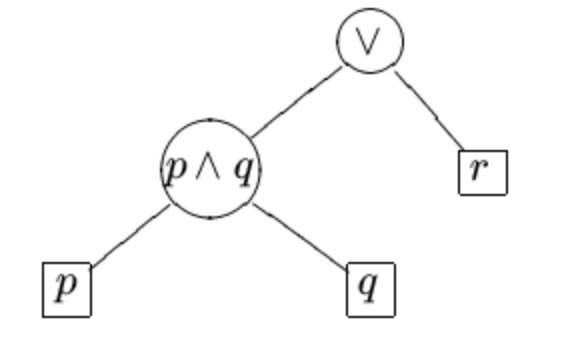
\includegraphics[width=0.8\textwidth]{2.3_1.jpg} % 插入图片
        \caption{测验题2.3 A选项}
    \end{minipage}
    \hfill
	%   \hspace{0.1\textwidth} % 调整这里的值来改变两张图片之间的间距
    \begin{minipage}[t]{0.45\textwidth}
        \centering
        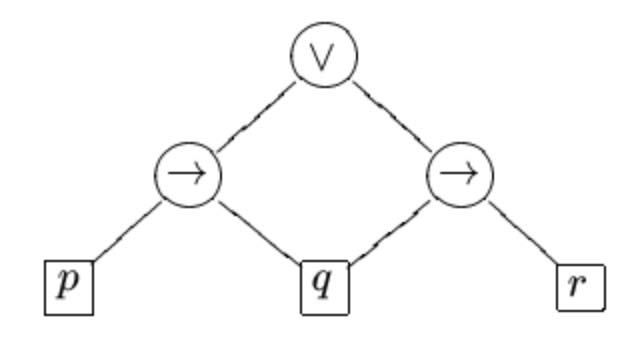
\includegraphics[width=0.8\textwidth]{2.3_2.jpg} % 插入图片
        \caption{测验题2.3 B选项}
\end{minipage}
\end{figure}

\clearpage

\begin{figure}[htbp]
  \centering
  \begin{minipage}[t]{0.45\textwidth}
      \centering
      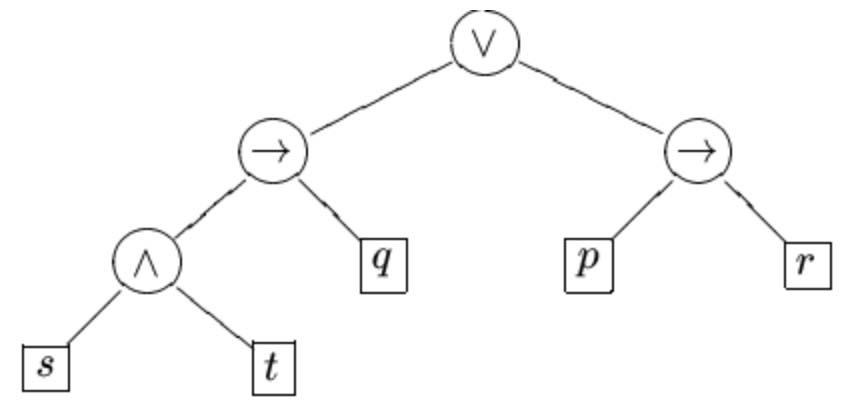
\includegraphics[width=0.9\textwidth]{2.3_3.jpg} % 插入图片
      \caption{测验题2.3 C选项}
  \end{minipage}
  \hfill
%   \hspace{0.1\textwidth} % 调整这里的值来改变两张图片之间的间距
  \begin{minipage}[t]{0.45\textwidth}
      \centering
      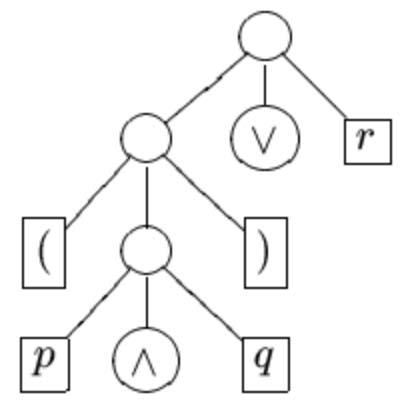
\includegraphics[width=0.6\textwidth]{2.3_4.jpg} % 插入图片
      \caption{测验题2.3 D选项}
\end{minipage}
\end{figure}

\textcolor{red}{答案:C}



\subsubsection{测验题2.4}

公式 $\neg(p \wedge q) \rightarrow(q \vee r)$ 是?

A. 否定式

B. 合取式

C. 蕴涵式

D. 析取式

\textcolor{red}{答案:C}

\subsubsection{测验题2.5}

公式 $r \vee s \leftrightarrow(q \rightarrow t) \wedge \neg r$ 是?

A. 合取式

B. 蕴涵式

C. 析取式

D. 双蕴涵式

\textcolor{red}{答案:D}

\subsubsection{测验题2.6}

公式 $((t \vee q) \wedge(q \leftrightarrow r) \rightarrow s) \wedge p$ 是?

A. 合取式

B. 蕴涵式

C. 析取式

D. 双蕴涵式

\textcolor{red}{答案:A}

\subsubsection{测验题2.7}

下面哪个公式不是公式 $\neg(p \wedge q) \rightarrow(q \wedge s \vee r))$ 的子公式? $\qquad$

A. $
p \wedge q
$

B. $
\neg p \wedge q
$

C. $
q \wedge s
$

D. $
q \wedge s \vee r
$

\textcolor{red}{答案:B}

\textcolor{red}{解析:注意子公式包含自身。}

\subsubsection{测验题2.8}

下面哪个公式是公式 $p \wedge q \rightarrow r \rightarrow s \vee t$ 的子公式?

A. $q \rightarrow r$

B. $r \rightarrow s$

C. $p \wedge q \rightarrow r$

D. $r \rightarrow s \vee t$

\textcolor{red}{答案:D}


\subsubsection{测验题2.9}

公式 $((\neg p) \wedge(q \vee((r \rightarrow s) \wedge(p \leftrightarrow q))))$ 总共有多少个不同的子公式?

A. 9

B. 10

C. 11

D. 12

\textcolor{red}{答案:B}

\subsubsection{测验题2.10}

公式 $(\neg(s \leftrightarrow t) \rightarrow q) \wedge(q \leftrightarrow r)$ 总共有多少个不同子公式?

A. 9

B. 10

C. 11

D. 12

\textcolor{red}{答案:A}

\subsubsection{测验题2.11}

给定 $\sigma$ 是真值赋值函数,$A, B$ 是任意的命题逻辑公式,下列说法不正确的是:

A.当 $\sigma(A)=1$ 时,$\sigma(A \wedge B)=\sigma(B)$ 。

B.当 $\sigma(A)=1$ 时,$\sigma(A \vee B)=1$ 。

C.当 $\sigma(A)=1$ 时,$\sigma(A \rightarrow B)=\sigma(B)$

D.当 $\sigma(B)=1$ 时,$\sigma(A \rightarrow B)=\sigma(A)$

\textcolor{red}{答案:D}

\subsubsection{测验题2.13}

给定命题变量 $p$ 和 $q$ 的真值, 计算公式 $(p \rightarrow q) \vee(\neg p \wedge \neg q)$ 的真值, 若要一次只考虑一个逻辑运算符, 则它的一些子公式按需要计算的顺序排列最合理的是 $\qquad$

A. $
p \rightarrow q, \quad \neg p, \quad \neg q, \quad \neg p \wedge \neg q
$

B. $
\neg p, \quad p \rightarrow q, \quad \neg p \wedge \neg q, \quad \neg q
$

C. $
\neg p \wedge \neg q, \quad \neg p, \quad \neg q, \quad p \rightarrow q
$

D. $
\neg p, \quad \neg q, \quad p \rightarrow q, \quad \neg q \wedge \neg p
$

\textcolor{red}{答案:A}

\textcolor{red}{解析:计算$p \rightarrow q$不需要知道 $\neg p$,D选项最后一个写反,还需要多使用一次交换律。}


\subsubsection{测验题2.14}

给定命题变量 $p, q, r, s$ 和 $t$ 的真值, 计算公式 $(r \wedge s \leftrightarrow q \vee p) \wedge(t \rightarrow r)$ 的真值, 若要一次只考虑一个逻辑运算符, 则它的一些子公式按需要计算的顺序排列最合理的是?

A. $\quad s \leftrightarrow q, \quad r \wedge s \leftrightarrow q, \quad r \wedge s \leftrightarrow q \vee p, \quad t \rightarrow r$

B. $\quad t \rightarrow r, \quad r \wedge s \leftrightarrow q \vee p, \quad r \wedge s \leftrightarrow q, \quad r \wedge s$

C. $\quad r \wedge s, \quad q \vee p, \quad r \wedge s \leftrightarrow q \vee p, \quad t \rightarrow r$

D. $\quad r \wedge s \leftrightarrow q \vee p, \quad r \wedge s, \quad q \vee p, \quad t \rightarrow r$


\textcolor{red}{答案:C}

\subsubsection{测验题2.15}

下面每个选项中的二进制串表示对命题变量 $p, q, r$ 依次赋值的一个真值赋值函数, 其中是公式 $(p \wedge q \rightarrow r \vee q) \wedge(p \leftrightarrow r)$ 的成真赋值有 $\qquad$

A. 000

B. 001

C. 101

D. 111

\textcolor{red}{答案:ACD}


\subsubsection{测验题2.16}

下面每个选项中的二进制串表示对命题变量 $p, q, r$ 依次斌值的一个真值赋值函数, 其中是公式 $(q \wedge p \leftrightarrow q \rightarrow r) \wedge(r \vee p)$ 的成假赋值有 $\qquad$

A. 000

B. 001

C. 101

D. 111

\textcolor{red}{答案:ABC}

\subsubsection{测验题2.17}

下面每个选项中的二进制串表示对命题变量 $p, q, r, s$ 依次赋值的一个真值赋值函数, 其中是公式 $(r \rightarrow s \leftrightarrow q \vee p) \wedge q \wedge p$ 的成真赋值有 $\qquad$

A. 0000

B. 0101

C. 1100

D. 1111

\textcolor{red}{答案:CD}

\subsubsection{测验题2.18}

下面每个选项中的二进制串表示对命题变量 $p, q, r, s$ 依次赋值的一个真值赋值函数, 其中是公式 $s \leftrightarrow \neg q \wedge r \wedge p$ 的成假赋值有 $\qquad$

A. 0000

B. 0101

C. 1100

D. 1111

\textcolor{red}{答案:BD}

\subsubsection{测验题2.19}

下面是公式 $(p \leftrightarrow q) \wedge(q \wedge p \rightarrow p \vee q)$ 的真值表,


\begin{table}[htbp]
\centering
\begin{tabular}{c|c|c|c|c|c|c}
\hline$p$ & $q$ & $p \leftrightarrow q$ & $q \wedge p$ & $p \vee q$ & $q \wedge p \rightarrow p \vee q$ & $(p \leftrightarrow q) \wedge(q \wedge p \rightarrow p \vee q)$ \\
\hline $\mathbf{0}$ & $\mathbf{0}$ & $(1)$ & $\mathbf{0}$ & $\mathbf{0}$ & $\mathbf{1}$ & $\mathbf{1}$ \\
\hline $\mathbf{0}$ & $\mathbf{1}$ & $\mathbf{0}$ & $\mathbf{0}$ & $(2)$ & $\mathbf{1}$ & $\mathbf{0}$ \\
\hline $\mathbf{1}$ & $\mathbf{0}$ & $\mathbf{0}$ & $\mathbf{0}$ & $\mathbf{1}$ & $(3)$ & $\mathbf{0}$ \\
\hline $\mathbf{1}$ & $\mathbf{1}$ & $\mathbf{1}$ & $\mathbf{1}$ & $\mathbf{1}$ & $\mathbf{1}$ & $\mathbf{( 4 )}$ \\
\hline
\end{tabular}
\end{table}

其中的空(1),(2),(3),(4) 依次填入的真值应该是:

A. 0000

B. 0101

C. 1100

D. 1111

\textcolor{red}{答案:D}

\subsubsection{测验题2.20}

下面是公式 $(p \wedge r \rightarrow q \vee r) \leftrightarrow \neg p$ 的真值表,
\begin{table}[htbp]
  \centering
\begin{tabular}{c|c|c|c|c|c|c|c}
\hline$p$ & $q$ & $r$ & $p \wedge r$ & $q \vee r$ & $p \wedge r \rightarrow q \vee r$ & $\neg p$ & $p \wedge r \rightarrow q \vee r \leftrightarrow \neg p$ \\
\hline $\mathbf{0}$ & $\mathbf{0}$ & $\mathbf{0}$ & $\mathbf{0}$ & $(1)$ & $\mathbf{1}$ & $\mathbf{1}$ & $\mathbf{1}$ \\
\hline $\mathbf{0}$ & $\mathbf{0}$ & $\mathbf{1}$ & $\mathbf{0}$ & $\mathbf{1}$ & $\mathbf{1}$ & $\mathbf{1}$ & $\mathbf{1}$ \\
\hline $\mathbf{0}$ & $\mathbf{1}$ & $\mathbf{0}$ & $\mathbf{0}$ & $\mathbf{1}$ & $\mathbf{1}$ & $\mathbf{1}$ & $\mathbf{1}$ \\
\hline $\mathbf{0}$ & $\mathbf{1}$ & $\mathbf{1}$ & $\mathbf{0}$ & $\mathbf{1}$ & $(2)$ & $\mathbf{1}$ & $(3)$ \\
\hline $\mathbf{1}$ & $\mathbf{0}$ & $\mathbf{0}$ & $\mathbf{0}$ & $\mathbf{0}$ & $\mathbf{1}$ & $\mathbf{0}$ & $\mathbf{0}$ \\
\hline $\mathbf{1}$ & $\mathbf{0}$ & $\mathbf{1}$ & $\mathbf{1}$ & $\mathbf{1}$ & $\mathbf{1}$ & $\mathbf{0}$ & $\mathbf{0}$ \\
\hline $\mathbf{1}$ & $\mathbf{1}$ & $\mathbf{0}$ & $\mathbf{0}$ & $\mathbf{1}$ & $\mathbf{1}$ & $\mathbf{0}$ & $(4)$ \\
\hline $\mathbf{1}$ & $\mathbf{1}$ & $\mathbf{1}$ & $\mathbf{1}$ & $\mathbf{1}$ & $\mathbf{1}$ & $\mathbf{0}$ & $\mathbf{0}$ \\
\hline
\end{tabular}
\end{table}

其中的空(1),(2),(3),(4)依次填入的真值应该是:

A. 0000

B. 0110

C. 1100

D. 0111

\textcolor{red}{答案:B}


\subsubsection{测验题2.23}

公式 $A$ 的一个替换实例是用公式 $B$ 去替换一个命题变量 $p$ 在 $A$ 中所有出现而得到的公式, 即若 $A, B$ 是公式, $p$ 是命题变量, 则 $A[B / p]$ 是 $A$ 的一个替换实例。下面说法不正确的是 $\qquad$

A. 永真式的任意替换实例仍然是永真式。

B. 永真式的否定是矛盾式,矛盾式的否定是永真式。

C. 矛盾式的任意替换实例仍然是矛盾式。

D. 可满足式的任意替换实例仍然是可满足式。

\textcolor{red}{答案:D}



\subsubsection{测验题2.25}

下面公式中是永真式的是?

A. $ \neg(r \rightarrow \neg q) \vee(p \rightarrow \neg r)$

B. $(\neg p \vee \neg q) \rightarrow(p \leftrightarrow \neg q)$

C. $(p \rightarrow q) \wedge(\neg p \rightarrow \neg q)$

D. $(p \rightarrow q \rightarrow r) \rightarrow(p \rightarrow q) \vee(q \rightarrow r)$

\textcolor{red}{答案:D}

\textcolor{red}{解析:注意运算符的优先级为:$\neg$ >  $\vee$ > $\wedge$ > $\rightarrow$ > $\leftrightarrow$,其中只有$\rightarrow$的结合性是从右到左。}

\subsubsection{测验题2.26}

下面公式中不是永真式的是?

A. $((p \vee q \rightarrow(p \leftrightarrow q))) \leftrightarrow(p \leftrightarrow q)$

B. $ r \vee((p \rightarrow r) \wedge(p \leftrightarrow q))$

C. $(\neg q \wedge(p \rightarrow q)) \rightarrow \neg p$

D. $((p \vee q) \wedge \neg p) \rightarrow q$

\textcolor{red}{答案:B}

\subsubsection{测验题2.27}

公式 $((p \rightarrow q) \rightarrow q \rightarrow p) \rightarrow q \rightarrow p$ 的 (语义) 类型是: $\qquad$

A. 永真式

B. 矛盾式

C. 非永真的可满足式

D. 无法判断

\textcolor{red}{答案:A}

\subsubsection{测验题2.28}

公式 $p \wedge(q \leftrightarrow(r \wedge p) \vee(q \rightarrow r))$ 的 (语义) 类型是: $\qquad$

A. 永真式

B.  矛盾式

C.   非永真的可满足式

D. 无法判断

\textcolor{red}{答案:C}

\subsubsection{测验题2.29}

下面哪个说法是不正确的?

A. 公式 $A$ 和 $B$ 逻辑等值, 则对它们中的命题变量践任何真值时, 这两个公式的真值都相同。

B. 公式 $A$ 和 $B$ 逻辑等值, 则 $A \rightarrow B$ 是永真式。

C. 公式 $A$ 和 $B$ 逻辑等值, 则 $A$ 和 $B$ 是相同的公式。

D. 公式 $A$ 和 $B$ 逻辑等值, 且公式 $B$ 和 $C$ 逻辑等值, 则 $A$ 和 $C$ 也逻辑等值。

\textcolor{red}{答案:C}

\subsubsection{测验题2.30}

下面哪个说法是正确的?

A. 要证明公式 $A$ 和 $B$ 逻辑等值, 必须将 $A$ 等值变换为公式 $B$ 。

B. 在等值变换时, 必须将公式 $A$ 的一个子公式 $B$ 的所有出现都置换为与 $B$ 等值的公式 $B^{\prime}$ 。

C. 要证明公式 $A$ 和 $B$ 逻辑等值, 只能使用等值演算或构造真值表的方法。

D. 如果公式 $A$ 和 $B$ 逻辑等值, 那么 $A \rightarrow C$ 和 $B \rightarrow C$ 也逻辑等值。

\textcolor{red}{答案:D}

\subsubsection{测验题2.31}

下面哪些是基本逻辑等值式模式分配律的实例?

A. $(p \vee q) \wedge(p \vee r) \equiv p \vee(q \wedge r)$

B. $(p \vee q) \wedge(r \vee q) \equiv(p \wedge r) \vee q$

C. $(p \vee q) \wedge(p \vee r) \equiv(p \vee q \vee p) \wedge(p \vee q \vee r)$

D. $(p \wedge q) \wedge(p \vee r) \equiv(p \wedge q \wedge p) \vee(p \wedge q \wedge r)$

\textcolor{red}{答案:ABD}

\subsubsection{测验题2.33}

下面哪些是基本逻辑等值式模式德摩尔根律的实例?

A. $
(p \wedge q) \equiv \neg(p \vee q)
$

B. $
\neg(p \wedge q \wedge r) \equiv \neg(p \wedge q) \vee \neg r
$

C. $
\neg p \wedge \neg(q \vee r) \equiv \neg(p \vee q \vee r)
$

D. $
\neg \neg(p \wedge q) \equiv \neg \neg p \vee \neg \neg q
$

\textcolor{red}{答案:BC}


\subsubsection{测验题2.34}

下面的等值演算中 (1),(2)处使用的基本逻辑等值式模式依次是:

\[
\begin{aligned}
    & (p \to r) \land (q \to r) \\
    \equiv & \, (\neg p \lor r) \land (\neg q \lor r) \hspace{4cm} \text{// \textcolor{blue}{ 蕴涵等值式}} \\
    \equiv & \, (\neg p \land \neg q) \lor r \hspace{4.85cm} \text{// \textcolor{blue}{(1)}} \\
    \equiv & \, \neg (p \lor q) \lor r \hspace{5.08cm} \text{// \textcolor{blue}{ 德摩尔根律}} \\
    \equiv & \, (p \lor q) \to r \hspace{5.125cm} \text{// \textcolor{blue}{ (2)}}
\end{aligned}
\]

\textcolor{red}{答案:(1)分配律 (2)蕴涵等值式}

\subsubsection{测验题2.35}

下面的等值演算中 (1), (2) 处使用的基本逻辑等值式模式依次是 \underline{\quad\quad\quad\quad}、 \underline{\quad\quad\quad\quad}:

\[
\begin{aligned}
    & (p \rightarrow r) \vee (q \rightarrow r) \\
    \equiv & (\neg p \vee r) \vee (\neg q \vee r) \quad \quad // \text{\textcolor{blue}{ 蕴涵等值式}} \\
    \equiv & (\neg p \vee \neg q) \vee (r \vee r) \quad \quad // \text{\textcolor{blue}{交换律、结合律}} \\
    \equiv & (\neg p \vee \neg q) \vee r \quad \quad \quad \quad \hspace{0.2cm} // \text{\textcolor{blue}{(1)}} \\
    \equiv & \neg (p \wedge q) \vee r \quad \quad \quad \quad \quad // \text{\textcolor{blue}{(2)}} \\
    \equiv & (p \wedge q) \rightarrow r \quad \quad \quad \quad \quad // \text{\textcolor{blue}{蕴涵等值式}} \\
\end{aligned}
\]

\textcolor{red}{答案:(1)幂等律 (2)德摩尔根律;德摩根律}

\subsubsection{测验题2.36}

下面的等值演算中 (1), (2)处使用的基本逻辑等值式模式依次是:

$$
\begin{aligned}
& \neg(r \vee(q \wedge(\neg r \rightarrow \neg p))) \\
& \equiv \neg(r \vee(q \wedge(r \vee \neg p)))  // \text { \textcolor{blue}{蕴涵等值式}} \\
& \equiv \neg(r \vee((q \wedge r) \vee(q \wedge \neg p))) \quad // \text { \textcolor{blue}{分配律} } \\
& \equiv \neg(r \vee(q \wedge \neg p)) \quad // \textcolor{blue}{(1)} \\
& \equiv \neg r \wedge \neg(q \wedge \neg p) \quad // \text { \textcolor{blue}{(2)} } \\
& \equiv \neg r \wedge(\neg q \vee \neg \neg p) \quad // \text { \textcolor{blue}{德摩尔根律} } \\
& \equiv \neg r \wedge(p \vee \neg q) \quad // \text { \textcolor{blue}{双重否定律、交换律} }
\end{aligned}
$$


\textcolor{red}{答案:(1)吸收律 (2)德摩尔根律;德摩根律}

\subsubsection{测验题2.37}

下面的等值演算中 $(1),(2)$ 处使用的基本逻辑等值式模式依次是:

$$
\begin{aligned}
& \neg(p \vee \neg q) \rightarrow(q \rightarrow r) \\
& \equiv(\neg p \wedge q) \rightarrow(q \rightarrow r) \quad / / \text { \textcolor{blue}{德摩尔根律、双重否定律}} \\
& \equiv(\neg p \wedge q) \rightarrow(\neg q \vee r) \quad / / \text { \textcolor{blue}{蕴涵等值式} } \\
& \equiv \neg(\neg p \wedge q) \vee(\neg q \vee r) \quad / / \quad \text { \textcolor{blue}{(1)} } \\
& \equiv(\neg \neg p \vee \neg q) \vee(\neg q \vee r) \quad / / \quad \text { \textcolor{blue}{(2)} } \\
& \equiv(p \vee \neg q) \vee(\neg q \vee r) \quad / / \text { \textcolor{blue}{双重否定律} } \\
& \equiv \neg q \vee(p \vee r) \quad / / \text {\textcolor{blue}{ 幂等律、交换律} } \\
& \equiv q \rightarrow(p \vee r) \quad / / \text { \textcolor{blue}{蕴涵等值式} }
\end{aligned}
$$

\textcolor{red}{答案:(1)蕴涵等值式 (2)德摩尔根律;德摩根律}


\subsubsection{测验题2.38}

下面哪一组的两个公式是逻辑等值的?

A. 公式 $(p \rightarrow q) \wedge p$ 和 $q$

B. 公式 $(p \vee q) \wedge q$ 和 $q$

C. 公式 $(p \wedge q) \wedge q$ 和 $q$

D. 公式 $(p \leftrightarrow q) \wedge p$ 和 $q$

\textcolor{red}{答案:B}

\subsubsection{测验题2.39}

下面哪一组的两个公式是逻辑等值的?

A. 公式 $(p \rightarrow q) \vee p$ 和 $q$

B. 公式 $(p \vee q) \vee q$ 和 $q$

C. 公式 $(p \wedge q) \vee q$ 和 $q$

D. 公式 $(p \leftrightarrow q) \vee p$ 和 $q$

\textcolor{red}{答案:C}

\subsubsection{测验题2.40}

下面哪一组的两个公式是逻辑等值的?

A. $\quad$ 公式 $\neg(p \rightarrow q)$ 和 $\neg p \rightarrow q$

B. 公式 $\neg(p \leftrightarrow q)$ 和 $\neg p \leftrightarrow q$

C. 公式 $\neg(p \rightarrow q)$ 和 $\neg p \rightarrow \neg q$

D. 公式 $\neg(p \leftrightarrow q)$ 和 $\neg p \leftrightarrow \neg q$

\textcolor{red}{答案:B}



\subsubsection{测验题2.41}

下面哪一组的两个公式是逻辑等值的?

A. 公式 $(p \wedge q) \leftrightarrow(p \wedge r)$ 和 $p \wedge(q \leftrightarrow r)$

B. 公式 $(p \vee q) \leftrightarrow(p \vee r)$ 和 $p \vee(q \leftrightarrow r)$

C. 公式 $(p \wedge q) \leftrightarrow r$ 和 $(p \leftrightarrow r) \wedge(q \leftrightarrow r)$

D. 公式 $(p \vee q) \leftrightarrow r$ 和 $(p \leftrightarrow r) \vee(q \leftrightarrow r)$

\textcolor{red}{答案:B}

\subsubsection{测验题2.42}

下面哪一组的两个公式不是逻辑等值的?

A. 公式 $p \rightarrow q$ 和 $\neg q \rightarrow \neg p$

B.  公式 $p \leftrightarrow q$ 和 $\neg q \leftrightarrow \neg p$

C. 公式 $p \rightarrow(q \rightarrow r)$ 和 $(p \rightarrow q) \rightarrow r$

D. 公式 $p \leftrightarrow(q \leftrightarrow r)$ 和 $(p \leftrightarrow q) \leftrightarrow r$

\textcolor{red}{答案:C}

\subsubsection{测验题2.44}

下面哪个说法不是正确的?

A. 析取范式是一个或多个简单合取式的析取。

B. 合取范式是一个或多个简单析取式的合取。

C. 每一个简单析取式都既是合取范式又是析取范式。

D. 每一个只含与、或、非逻辑运算符的公式不是析取范式就是合取范式。

\textcolor{red}{答案:D}

\textcolor{red}{解析:析取范式中的合取式都是\textbf{一个}或多个文字的合取;合取范式中的析取式都是\textbf{一个}或多个文字的析取。
因此$p \vee q$既是析取范式又是合取范式。}

\subsubsection{测验题2.46}

下面哪些公式是析取范式?

A. $ \neg p$

B. $\neg(p \vee q)$

C. $\neg p \wedge \neg q$

D. $ \neg p \vee \neg q$

\textcolor{red}{答案:ACD}

\subsubsection{测验题2.48}

下面哪些公式是析取范式?

A. $\neg(p \wedge q) \vee r$

B. $\quad(\neg p \wedge q) \vee r$

C. $\quad(\neg p \vee q) \wedge r$

D. $\quad(\neg p \wedge q) \vee(p \vee r)$

\textcolor{red}{答案:BD}


\subsubsection{测验题2.49}

下面哪些公式是合取范式?

A. $ \neg(p \vee q) \wedge r$

B. $(\neg p \wedge q) \vee r$

C. $(\neg p \wedge q) \wedge r$

D. $(\neg p \wedge q) \vee(p \vee r)$

\textcolor{red}{答案:C}

\subsubsection{测验题2.50}

下面哪些公式是与公式 $p \leftrightarrow q$ 逻辑等值的析取范式?

A. $\neg(p \vee q) \vee(p \wedge q)$

B. $(\neg p \wedge q) \vee(p \wedge \neg q)$

C. $(\neg p \vee q) \wedge(p \vee \neg q)$

D. $(\neg p \wedge \neg q) \vee(p \wedge q)$

\textcolor{red}{答案:D}

\subsubsection{测验题2.51}

下面哪些公式是与公式 $p \leftrightarrow q$ 逻辑等值的合取范式?

A. $\neg(p \vee q) \vee(p \wedge q)$

B. $(\neg p \wedge q) \vee(p \wedge \neg q)$

C. $(\neg p \vee q) \wedge(p \vee \neg q)$

D. $(\neg p \wedge \neg q) \vee(p \wedge q)$

\textcolor{red}{答案:C}

\subsubsection{测验题2.53}

下面哪些公式是与公式 $(p \rightarrow q) \rightarrow r$ 逻辑等值的合取范式?

A. $ \neg p \vee \neg q \vee r$

B. $(p \wedge \neg q) \vee r$

C. $(p \vee r) \wedge(\neg q \vee r)$

D. $(\neg p \wedge q) \vee r$

\textcolor{red}{答案:C}

\subsubsection{测验题2.55}

下面哪些说法不是正确的?

A. 每个命题逻辑公式既存在与之等值的主合取范式,也存在与之等值的主析取范式

B. 极小项的编码是使得这个极小项的真值为真的唯一的真值赋值方式

C.设有 3 个命题变量,极小项 $m_2$ 的否定与 $M_2$ 逻辑等值。

D.与主析取范式 $m_1 \vee m_3 \vee m_5$ 逻辑等值的主合取范式是 $M_1 \wedge M_3 \wedge M_5$ 。

\textcolor{red}{答案:D}

\subsubsection{测验题2.57}

设公式含 $p, q, r$ 三个命题变量, 下面哪些公式是极大项?

A. $ p \vee \neg q \vee r$

B. $ p \wedge \neg q \wedge r$

C. $ p \wedge r$

D. $ p \vee r$

\textcolor{red}{答案:A}

\textcolor{red}{解析:合取极小项,析取极大项(可以看第一个字的笔画数来记忆)。}

\subsubsection{测验题2.58}

设公式含 $p, q, r, s$ 四个命题变量, 且极小项编码遵循 $p, q, r, s$ 的顺序。下面哪些极小项会包含在简单合取式 $\neg q \wedge \neg s$ 扩展得到的主析取范式中?

A. $ m_2$

B. $m_4$

C. $ m_6$

D. $ m_8$

\textcolor{red}{答案:AD}

\textcolor{red}{解析:主析取范式为$m$,例如$p \overline{q} r \overline{s}$为$m_{10}$;
主合取范式为$M$。}

\subsubsection{测验题2.59}

设公式含 $p, q, r, s$ 四个命题变量, 
且极小项编码遵循 $p, q, r, s$ 的顺序。
下面哪些极小项会包含在简单合取式 $\neg p \wedge r$ 
扩展得到的主析取范式中?

A. $ m_1$

B. $m_3$

C. $ m_5$

D. $ m_7$

\textcolor{red}{答案:BD}


\subsubsection{测验题2.61}

设公式含 $p, q, r, s$ 四个命题变量, 且极大项编码遵循 $p, q, r, s$ 的顺序。下面哪些极大项会包含在简单析取式 
$\neg p \vee r$ 扩展得到的主合取范式中?

A. $ M_8$

B. $M_{10}$

C. $ M_{12}$

D. $ M_{16}$

\textcolor{red}{答案:AC}

\subsubsection{测验题2.63}

与公式 $((p \vee q) \rightarrow r) \rightarrow q$ 逻辑等值的主范式有 $\qquad$

A. $\quad m_0 \vee m_1 \vee m_5$

B. $\quad m_2 \vee m_3 \vee m_4 \vee m_6 \vee m_7$

C. $\quad M_0 \wedge M_1 \wedge M_5$

D. $\quad M_2 \vee M_3 \vee M_4 \vee M_6 \vee M_7$

\textcolor{red}{答案:BC}

\subsubsection{测验题2.64}

下面是公式 $(p \rightarrow r) \wedge(\neg r \rightarrow q)$ 的真值表,

\begin{table}[htbp]
  \centering
\begin{tabular}{c|c|c|c|c|c|c}
\hline$p$ & $q$ & $r$ & $p \rightarrow r$ & $\neg r$ & $\neg r \rightarrow q$ & $(p \rightarrow r) \wedge(\neg r \rightarrow q)$ \\
\hline $\mathbf{0}$ & $\mathbf{0}$ & $\mathbf{0}$ & $\mathbf{1}$ & $\mathbf{1}$ & $\mathbf{0}$ & $\mathbf{0}$ \\
\hline $\mathbf{0}$ & $\mathbf{0}$ & $\mathbf{1}$ & $\mathbf{1}$ & $\mathbf{0}$ & $\mathbf{1}$ & $\mathbf{1}$ \\
\hline $\mathbf{0}$ & $\mathbf{1}$ & $\mathbf{0}$ & $\mathbf{1}$ & $\mathbf{1}$ & $\mathbf{1}$ & $\mathbf{1}$ \\
\hline $\mathbf{0}$ & $\mathbf{1}$ & $\mathbf{1}$ & $\mathbf{1}$ & $\mathbf{0}$ & $\mathbf{1}$ & $\mathbf{1}$ \\
\hline $\mathbf{1}$ & $\mathbf{0}$ & $\mathbf{0}$ & $\mathbf{0}$ & $\mathbf{1}$ & $\mathbf{0}$ & $\mathbf{0}$ \\
\hline $\mathbf{1}$ & $\mathbf{0}$ & $\mathbf{1}$ & $\mathbf{1}$ & $\mathbf{0}$ & $\mathbf{1}$ & $\mathbf{1}$ \\
\hline $\mathbf{1}$ & $\mathbf{1}$ & $\mathbf{0}$ & $\mathbf{0}$ & $\mathbf{1}$ & $\mathbf{1}$ & $\mathbf{0}$ \\
\hline $\mathbf{1}$ & $\mathbf{1}$ & $\mathbf{1}$ & $\mathbf{1}$ & $\mathbf{0}$ & $\mathbf{1}$ & $\mathbf{1}$ \\
\hline
\end{tabular}
\end{table}

则与该公式等值的主范式是

A. $
m_1 \wedge m_2 \wedge m_3 \wedge m_5 \wedge m_7
$

B. $m_0 \wedge m_4 \wedge m_6$

C. $m_1 \vee m_2 \vee m_3 \vee m_5 \vee m_7$

D. $m_0 \vee m_4 \vee m_6$

\textcolor{red}{答案:C}

\subsubsection{测验题2.65}

下面是公式 $(p \rightarrow r) \wedge(\neg r \rightarrow q)$ 的真值表。
\begin{table}[htbp]
  \centering
\begin{tabular}{c|c|c|c|c|c|c}
\hline$p$ & $q$ & $r$ & $p \rightarrow r$ & $\neg r$ & $\neg r \rightarrow q$ & $(p \rightarrow r) \wedge(\neg r \rightarrow q)$ \\
\hline 0 & 0 & 0 & 1 & 1 & 0 & 0 \\
\hline 0 & 0 & 1 & 1 & 0 & 1 & 1 \\
\hline 0 & 1 & 0 & 1 & 1 & 1 & 1 \\
\hline 0 & 1 & 1 & 1 & 0 & 1 & 1 \\
\hline 1 & 0 & 0 & 0 & 1 & 0 & 0 \\
\hline 1 & 0 & 1 & 1 & 0 & 1 & 1 \\
\hline 1 & 1 & 0 & 0 & 1 & 1 & 0 \\
\hline 1 & 1 & 1 & 1 & 0 & 1 & 1 \\
\hline
\end{tabular}
\end{table}

则与该公式等值的主范式是

A. $
M_1 \wedge M_2 \wedge M_3 \wedge M_5 \wedge M_7
$

B. $
M_0 \wedge M_4 \wedge M_6
$

C. $
M_1 \vee M_2 \vee M_3 \vee M_5 \vee M_7
$

D. $
M_0 \vee M_4 \vee M_6
$

\textcolor{red}{答案:B}

\subsubsection{测验题2.66}

下面哪个说法是不正确的?

A. 如果推理 $A_1, \cdots, A_n \Longrightarrow B$ 是有效的,则公式 $A_1 \wedge \cdots \wedge A_n \rightarrow B$ 是永真式。

B.   如果推理 $A_1, \cdots, A_n \Longrightarrow B$ 是有效的, 则公式 $B$ 的真值一定为真。

C.    如果 $B$ 是永真式, 则推理 $A_1, \cdots, A_n \Longrightarrow B$ 是有效的。

D. 如果 $B$ 不是永真式, 则推理 $A_1, \cdots, A_n \Longrightarrow B$ 不可能是有效的。


\textcolor{red}{答案:BD}

\subsubsection{测验题2.67}

下面哪些说法是不正确的?

A. 由前提"如果2020年是闰年, 则2021年是闰年"和前提"2020年是闰年", 推出结论"2021年是闰年"的推理是有效的。

B. 由前提"如果2020年是闰年,则2021年是闰年"和前提"2020年不是闰年",推出结论"2021年不是闰年"的推理是有效的。

C. 由前提"如果2020年是闰年,则2021年是闰年"和前提"2021年不是闰年",推出结论"2020年不是闰年"的推理是有效的。

D. 由前提"如果2020年是闰年,则2021年是闰年"和前提"2021年是闰年",推出结论"2020年是闰年"的推理是有效的。

\textcolor{red}{答案:BD}

\subsubsection{测验题2.68}

从前提"如果2020年是闰年, 则2021年不是闰年"和前提"2020年是闰年", 推出结论"2021年不是闰年"使用的推理规则是

A. 假言推理

B. 假言易位

C. 附加规则

D. 析取三段论

\textcolor{red}{答案:A}

\subsubsection{测验题2.69}

从前提“如果2020年是闰年,则2021年不是闰年”和前提“2021年是闰年”,推出结论“2020年不是闰年”使用的推理规则是

A. 假言推理

B. 假言易位

C. 附加规则

D. 析取三段论

\textcolor{red}{答案:B}

\subsubsection{测验题2.70}

从前提“2020年是闰年而且2021年不是闰年”推出结论“2021年不是闰年”使用的推理规则是

A. 假言推理

B. 假言易位

C. 合取规则

D. 化简规则

\textcolor{red}{答案:D}


\subsubsection{测验题2.71}

从前提"2020年是闰年"和前提"2021年不是闰年"推出结论"2020年是闰年而且2021年不是闰年"使用的推理规则是

A. 假言推理

B. 假言易位

C. 合取规则

D. 化简规则

\textcolor{red}{答案:C}

\subsubsection{测验题2.72}

从前提"或者2020年是闰年, 或者2021年是闰年"和前提"2021年不是闰年", 推出结论"2020年是闰年"使用的推理规则是

A. 假言推理

B. 假言易位

C. 附加规则

D. 析取三段论

\textcolor{red}{答案:D}

\subsubsection{测验题2.76}

下面是验证推理 $p \rightarrow(q \rightarrow s), \neg r \vee p, q \Longrightarrow r \rightarrow s$ 有效性的论证:

\begin{table}[htbp]
  \centering
  \renewcommand{\arraystretch}{1.5}
\begin{tabular}{ll} 
(1) $r$ & $/ /$ \textcolor{blue}{附加前提} \\
(2) $\neg r \vee p$ & $/ /$ \textcolor{blue}{前提} \\
(3) $p$ & $/ /$ \textcolor{blue}{(1),(2)析取三段论} \\
(4) $p \rightarrow(q \rightarrow s)$ & $/ /$ \textcolor{blue}{前提} \\
(5) $q \rightarrow s$ & $/ /$ \textcolor{blue}{(3),(4)假言推理} \\
(6) $q$ & $/ /$ \textcolor{blue}{前提} \\
(7) $s$ & $/ /$ \textcolor{blue}{(5),(6)假言推理} \\
(8) $r \rightarrow s$ & $/ /$ \textcolor{blue}{(1),(7)附加前提法}
\end{tabular}
\end{table}

记公式 $H$ 是前提的合取, 即 $H$ 是 $(p \rightarrow(q \rightarrow s)) \wedge(\neg r \vee p) \wedge q$, 下面咈些说法是正确的?

A. 由上面(1)可得到公式 $H \rightarrow r$ 是永真式。

B. 由上面 (3)可得到公式 $H \rightarrow p$ 是永真式。

C. 由上面 $(5)$ 可得到公式 $(H \wedge r) \rightarrow(q \rightarrow s)$ 是永真式。

D. 由上面 (8) 可得到公式 $H \rightarrow(r \rightarrow s)$ 是永真式。

\textcolor{red}{答案:CD}

\subsubsection{测验题2.77}

下面是验证推理 $s \rightarrow \neg q, r \vee s, \neg q \vee \neg r \Longrightarrow \neg q$ 有效性的论证:
\begin{table}[htbp]
  \centering
  \renewcommand{\arraystretch}{1.5}
\begin{tabular}{ll} 
(1) $q$ & $/ /$ \textcolor{blue}{附加前提} \\
(2) $s \rightarrow \neg q$ & $/ /$ \textcolor{blue}{前提} \\
(3) $\neg s$ & $/ /$\textcolor{blue}{(1),(2) 假言易位} \\
(4) $r \vee s$ & $/ /$ \textcolor{blue}{前提} \\
(5) $r$ & $/ /$\textcolor{blue}{(3),(4) 析取三段论} \\
(6) $\neg q \vee \neg r$ & $/ /$ \textcolor{blue}{前提} \\
(7) $\neg r$ & $/ /$\textcolor{blue}{(1),(6) 析取三段论} \\
(8) $\neg q$ & $/ /$\textcolor{blue}{(1),(5),(7) 反证法}
\end{tabular}
\end{table}

记公式 $H$ 是前提的合取, 即 $H$ 是 $(s \rightarrow \neg q) \wedge(r \vee s) \wedge(\neg q \vee \neg r)$, 下面哪些说法是正确的?

A. 上面 (5)给出的公式 $r$ 是由 $\neg s$ 和 $r \vee s$ 通过析取三段论规则得到的。

B. 由上面 $(3)$ 可得到公式 $H \rightarrow \neg s$ 是永真式。

C. 由上面 $(5)$ 可得到公式 $(H \wedge q) \rightarrow r$ 是永真式。

D. 由上面 (8)可得到公式 $H \rightarrow \neg q$ 是永真式。

\textcolor{red}{答案:ACD}

\textcolor{red}{解析:B选项应为$(H \wedge q) \rightarrow \neg s$。}

\subsubsection{测验题2.78}
下面是验证推理  $\neg(p \rightarrow q) \rightarrow \neg(r \vee s),(q \rightarrow p) \vee \neg r, r \Longrightarrow p \leftrightarrow q$ 有效性的论证:

\[
\begin{aligned}
(1) & \quad r \hspace{5cm} \text{// \textcolor{blue}{前提}} \\
(2) & \quad (q \to p) \vee \neg r \hspace{3.1cm} \text{// \textcolor{blue}{前提}} \\
(3) & \quad q \to p \hspace{4.2cm} \text{// {\textcolor{blue}{(a)}}} \\
(4) & \quad r \vee s \hspace{4.35cm} \text{// \textcolor{blue}{(1) 附加规则}} \\
(5) & \quad \neg(p \to q) \to \neg(r \vee s) \hspace{1.8cm} \text{// \textcolor{blue}{前提}} \\
(6) & \quad p \to q \hspace{4.2cm} \text{// {\textcolor{blue}{(b)}}} \\
(7) & \quad (p \to q) \land (q \to p) \hspace{2.3cm} \text{// \textcolor{blue}{(3), (6) 合取规则}} \\
(8) & \quad p \leftrightarrow q \hspace{4.2cm} \text{// \textcolor{blue}{(7) 双蕴涵逻辑等值式}}
\end{aligned}
\]

其中(a),(b)两个空应该依次填写?

\textcolor{red}{答案:(a)(1),(2)析取三段论 (b)(4),(5)假言易位}

\subsubsection{测验题2.79}

下面是验证推理 $\neg(p \land q), \, q \lor r, \, \neg r \implies \neg p$ 有效性的论证:

\[
\begin{array}{rl}
(1) & p \quad \quad // \textcolor{blue}{\text{附加前提}} \\
(2) & \neg r \quad \quad // \textcolor{blue}{\text{前提}} \\
(3) & q \lor r \quad \quad // \textcolor{blue}{\text{前提}} \\
(4) & q \quad \quad // \textcolor{blue}{\text{(a)}} \\
(5) & p \land q \quad \quad // \textcolor{blue}{\text{(1), (4) 合取规则}} \\
(6) & \neg(p \land q) \quad \quad // \textcolor{blue}{\text{前提}} \\
(7) & \neg p \quad \quad // \textcolor{blue}{\text{(b)}}
\end{array}
\]

其中 (a),(b)两个空应该依次填写?

\textcolor{red}{答案:(a)(2),(3)析取三段论 (b)(1),(5),(6)反证法}

\subsubsection{测验题2.80}

下面是验证推理 $\neg r \rightarrow(\neg p \vee s), q \rightarrow \neg s \Longrightarrow p \rightarrow(q \rightarrow r)$ 有效性的论证:

\[
\begin{aligned}
    (1) & \quad p \quad \quad \quad \quad \quad \quad \quad \quad \quad // \text{\textcolor{blue}{附加前提}} \\
    (2) & \quad q \quad \quad \quad \quad \quad \quad \quad \quad \quad // \text{\textcolor{blue}{附加前提}} \\
    (3) & \quad q \rightarrow \neg s \quad \quad \quad \quad \quad \quad // \text{\textcolor{blue}{前提}} \\
    (4) & \quad \neg s \quad \quad \quad \quad \quad \quad \quad \quad // \text{ \textcolor{blue}{(2), (3)假言推理}} \\
    (5) & \quad \neg r \quad \quad \quad \quad \quad \quad \quad \quad // \text{\textcolor{blue}{附加前提}} \\
    (6) & \quad \neg r \rightarrow (\neg p \vee s) \quad \quad \quad // \text{\textcolor{blue}{前提}} \\
    (7) & \quad \neg p \vee s \quad \quad \quad \quad \quad \quad \hspace{0.2cm} // \text{ \textcolor{blue}{(5), (6)假言推理}} \\
    (8) & \quad \neg p \quad \quad \quad \quad \quad \quad \quad \quad // \text{ \textcolor{blue}{(4), (7)析取三段论}} \\
    (9) & \quad r \quad \quad \quad \quad \quad \quad \quad \quad \quad // \, \textcolor{blue}{(a)} \\
    (10) & \quad q \rightarrow r \quad \quad \quad \quad \quad \quad \hspace{0.3cm} // \text{ \textcolor{blue}{(2), (9)附加前提法}} \\
    (11) & \quad p \rightarrow (q \rightarrow r) \quad \quad \quad \hspace{0.3cm} // \, \textcolor{blue}{(b)} \\
\end{aligned}
\]

其中 (a),(b)两个空应该依次填写?

\textcolor{red}{答案:(a)(1),(5),(8)反证法 (b)(1),(10)附加前提法}

\subsubsection{测验题2.81}

下面哪些是命题?

A. C++语言是一门难学的程序设计语言。

B. C++语言真难学啊!

C. C++语言真的很难学吗?

D. 只要你认真学习,C++语言就不是难学的程序设计语言。

\textcolor{red}{答案:AD}

\subsubsection{测验题2.84}

设 $p$ 表示 "学生学过C++语言", $q$ 表示 "学生学过Java语言"。命题 "学生只要学过C++语言,就会学过Java语言" 符号化为?

A. $ p \rightarrow q$

B. $ q \rightarrow p$

C. $ p \wedge q$

D. $ p \vee q$

\textcolor{red}{答案:A}

\subsubsection{测验题2.85}

设 $p$ 表示"学生学过C++语言", $q$ 表示 "学生学过Java语言"。命题 "学生只有学过C++语言,才会学过Java语言" 符号化为 $\qquad$

A. $
p \rightarrow q
$

B. $
q \rightarrow p
$

C. $
p \wedge q
$

D. $
p \vee q
$

\textcolor{red}{答案:B}

\subsubsection{测验题2.86}

设 $p$ 表示 "学生学过C++语言", $q$ 表示 "学生学过Java语言", $r$ 表示 "学生理解面向对象编程思想",命题 "学生不仅学过C++语言,而且学过Java语言,但并不理解面向对象编程思想" 符号化为

A. $
(p \vee q) \rightarrow \neg r
$

B. $
(p \wedge q) \rightarrow \neg r
$

C. $
p \wedge q \wedge \neg r
$

D. $
(p \wedge q) \vee \neg r
$

\textcolor{red}{答案:C}



\subsubsection{测验题2.87}

设 $p$ 表示 "学生学过C++语言", $q$ 表示 "学生学过Java语言", $r$ 
表示 "学生理解面向对象编程思想"。命题 "学生学过C++语言或Java语言, 
但并不理解面向对象编程思想" 符号化为?

A. $(p \vee q) \rightarrow \neg r$

B. $(p \wedge q) \rightarrow \neg r$

C. $(p \vee q) \wedge \neg r$

D. $(p \wedge q) \vee \neg r$

\textcolor{red}{答案:C}

\textcolor{red}{解析:注意“虽然但是”表示的是合取关系。}

\subsubsection{测验题2.88}

设 $p$ 表示 "学生学过C ++ 语言", $q$ 表示 "学生学过Java语言", $r$ 表示 
"学生理解面向对象编程思想"。命题 "学生不理解面向对象编程思想,
除非学过C++语言或Java语言"符号化为?

A. $
(p \vee q) \rightarrow \neg r
$

B. $
(p \vee q) \rightarrow r
$

C. $
\neg r \rightarrow(p \vee q)
$

D. $
r \rightarrow(p \vee q)
$

\textcolor{red}{答案:D}


\subsubsection{测验题2.89}

设 $p$ 表示 "学生学过C++语言", $q$ 表示 "学生学过Java语言", $r$ 表示
 "学生理解面向对象编程思想"。命题 "如果学生没有学过C++语言或Java语言, 
 那么他不理解面向对象编程思想" 符号化为?

A. $(\neg p \vee \neg q) \rightarrow \neg r$

В、 $\neg(p \vee q) \rightarrow \neg r$

C. $(\neg p \vee q) \rightarrow \neg r$

D. $ p \vee q \rightarrow r$

\textcolor{red}{答案:B}

\subsubsection{测验题2.90}

设 $p$ 表示 "学生学过C ++ 语言", $q$ 表示 "学生学过Java语言", $r$ 表示 
"学生理解面向对象编程思想"。命题 "除非既学过C++语言又学过Java语言, 
否则学生不理解面向对象编程思想" 符号化为?

A. $(p \wedge q) \rightarrow \neg r$

B. $(p \wedge q) \rightarrow r$

C. $ \neg r \rightarrow(p \wedge q)$

D. $ r \rightarrow(p \wedge q)$

\textcolor{red}{答案:D}

\subsubsection{测验题2.91}

设 $p$ 表示 "学生学过C++语言", $q$ 表示 "学生学过Java语言", $r$ 表示 "学生理解面向对象编程思想"。命题 "学生学过C++语言, 而且如果他还学过Java语言, 那么他理解面向对象编程思想" 符号化为 $\qquad$。

A. $\quad p \wedge(q \rightarrow r)$

B. $\quad(p \wedge q) \rightarrow r$

C. $\quad p \wedge q \wedge r$

D. $\quad p \rightarrow(q \rightarrow r)$

\textcolor{red}{答案:A}  

\subsubsection{测验题2.93}

设 $p$ 表示 "学生学过C++语言", $q$ 表示 "学生学过Java语言", 
$r$ 表示 "学生理解面向对象编程思想"。命题 "学生如果学过C++语言, 
则他理解面向对象编程思想, 除非他没有学过Java语言" 符号化为?

A. $(p \rightarrow r) \rightarrow \neg q$

B. $\neg(p \rightarrow r) \rightarrow \neg q$

C. $\neg q \rightarrow(p \rightarrow r)$

D. $\ \neg q \rightarrow \neg(p \rightarrow r)$

\textcolor{red}{答案:B}

\textcolor{red}{解析:\textit{p除非q} 等价于 \textit{除非q否则p} 等价于 \textit{除非q才非p} 
等价于$\neg p\rightarrow q$。借用汉语词典的例子:
\begin{enumerate}
  \item \textcolor{red}{除非在这里修个水库,否则不能解决供水问题。}
  \item \textcolor{red}{不能解决供水问题,除非在这里修个水库。}
  \item \textcolor{red}{除非在这里修个水库,才能解决供水问题。}
\end{enumerate}
解决了供水问题可以推出修建了水库,因此是$\neg p\rightarrow q$;但是不能保证修了水库就能解决供水问题。
记忆:除非后面的东西是蕴涵式的后件。
}

\subsubsection{测验题2.94}

命题“如果学生学过C++语言, 则他理解面向对象编程思想”题是?

A. “如果学生没学过C++语言, 则他不理解面向对象编程思想”

B. “如果学生理解面向对象编程思想, 则他学过C++语言”

C. “如果学生不理解面向对象编程思想, 则他没学过C++语言”

D. “只要学生学过C++语言, 他就理解面向对象编程思想”

\textcolor{red}{答案:B}

\subsubsection{测验题2.96}

命题“如果学生学过C++语言,则他理解面向对象编程思想”的逆否命题是?

A. "如果学生没学过C++语言, 则他不理解面向对象编程思想"

B. "如果学生理解面向对象编程思想,则他学过C++语言"

C. "如果学生不理解面向对象编程思想, 则他没学过C++语言"

D. "只要学生学过C++语言, 他就理解面向对象编程思想"

\textcolor{red}{答案:C}

\subsubsection{测验题2.100}

学校要从程序设计竞赛集训队赵、钱、孙、李、周五人中挑选若干人组队参加下次的国际程序设计竞赛,经过考察平时配合情况,发现:(1) 如果赵去,则钱也去;(2) 周和李两人中至少去一人;(3) 钱和孙去且仅去一人;(4) 孙、李同去或同不去;(5) 若周去,则赵和钱都去。

分别使用p, q, r, s, t表示原子命题“赵/钱/孙/李/周去参加竞赛”,并按照p,q,r,s,t的顺序对范式中的极大项或极小项进行编码。那么将描述可能组队方案的公式展开为主范式,会包含下面哪些项?

A. $ m_{30}$

B. $ m_{22}$

C. $ m_{25}$

D. $ m_{28}$

\textcolor{red}{答案:C}


\clearpage
\section{一阶逻辑}

\subsubsection{测验题3.1}

假设为研究自然数性质提取了常量符号 0,1 , 运算符号,$+ *$, 关系符号 $=, \geq$, 并使用变量符号 $x, y, z$, 逻辑运算符 $\neg, \wedge, \vee, \rightarrow$, 量词符号 $\forall, \exists$ 。这些符号中讲些是非逻辑符号?

A. 关系符号 $=, \geq$

B.变量符号 $x, y, z$

C. 运算符号,$+ *$

D. 量词符号 $\forall, \exists$

\textcolor{red}{答案:AC}

\textcolor{red}{解析:一阶逻辑公式中出现的逻辑符号包括: (1) 个体变量符号, 使用小写字母 $x, y, z, \cdots$ 等表示个体变量, 记所有个体变量符号构成的集合为$V$;
(2)逻辑运算符号,包括否定 $\neg$ 逻辑与 $\wedge$ 、
逻辑或 $\vee$ 、逻辑蕴涵 $\rightarrow$ 和逻辑双蕴涵 
$\leftrightarrow ;(3)$ 量词符号:包括全称量词 $\forall$ 
和存在量词 $\exists ;(4)$ 辅助符号,包括圆括号(和), 以及逗号。
\\ 一阶逻辑公式中出现的非逻辑符号包括:(1)个体常量符号,
使用小写字母 $a, b, c, \cdots$ 等表示个体常量;(2)函数符号,
使用小写字母 $f, g, h, \cdots$ 等表示函数,每个函数都有一个元数信息,
表明该函数是几元函数;(3)谓词符号,使用大写字母 $F, G, H, \cdots$ 表示谓词,
每个谓词都有一个元数信息,表明该谓词是几元谓词。}

\subsubsection{测验题3.2}

假设为研究自然数性质提取了常量符号 0,1 , 运算符号,$+ *$, 关系符号 $=, \geq$, 并使用变量符号 $x, y, z$, 逻辑运算符 $\neg, \wedge, \vee, \rightarrow$, 量词符号 $\forall, \exists$ 。这些符号中哪些是逻辑符号?

A. 关系符号 $=, \geq$

B. 变量符号 $x, y, z$

C. 运算符号,$+ *$

D. 量词符号 $\forall, \exists$

\textcolor{red}{答案:BD}


\subsubsection{测验题3.3}

假设为研究自然数性质提取了常量符号 0,1 , 运算符号,$+ *$, 关系符号 $=, \geq$, 并使用变量符号 $x, y, z$, 逻辑运算符 $\neg, \wedge, \vee, \rightarrow$, 量词符号 $\forall, \exists$ 。下面呀些是一阶逻辑公式中的项?

A. $ x+1$

B. $ x \geq 0$

C. $\forall x(x \geq 0)$

D. $ x *(y+z)$

\textcolor{red}{答案:AD}

\subsubsection{测验题3.5}

下面哪些公式是一阶逻辑公式 $\forall x \exists y(x+y \geq 0) \rightarrow \exists x(\forall y(x * y=x) \wedge \forall z(x+z=z))$ 的子公式?

A. $
x+y
$


B. $
\exists y(x+y \geq 0)
$


C. $
\exists x \forall y(x * y=x)
$


D. $
x+z=z
$

\textcolor{red}{答案:BD}

\subsubsection{测验题3.6}

下面哪些公式是一阶逻辑公式 $\forall x(F(x) \wedge H(x, y)) \rightarrow \exists x(G(x, y) \rightarrow(\neg \exists y H(x, y)))$ 的子公式?

A. $
\forall x F(x)
$


B. $
\exists x G(x, y)
$

C. $
H(x, y)
$

D. $
G(x, y) \rightarrow(\neg \exists y H(x, y))
$

\textcolor{red}{答案:CD}




\subsubsection{测验题3.7}

一阶逻辑公式 $\forall x \exists y(x+y \geq 0) \rightarrow \exists x(\forall y(x * y=x) \wedge \forall z(x+z=z))$ 中量词 $\forall x$ 的辖域是 $\qquad$

A. $\forall x \exists y(x+y \geq 0)$

B. $ \exists y(x+y \geq 0) \rightarrow \exists x(\forall y(x * y=x) \wedge \forall z(x+z=z))$

C. $\exists y(x+y \geq 0)$

D. $(x+y \geq 0)$

\textcolor{red}{答案:C}

\subsubsection{测验题3.8}

一阶逻辑公式 $\forall x \exists y(x+y \geq 0) \rightarrow \exists x(\forall y(x * y=x) \wedge \forall z(x+z=z))$ 中量词 $\exists x$ 的辖域是 $\qquad$

A. $ \forall y(x * y=x)$

B. $\forall y(x * y=x) \wedge \forall z(x+z=z)$

C. $\forall z(x+z=z)$

D. $(x * y=x)$ 和 $(x+z=z)$

\textcolor{red}{答案:B}

\subsubsection{测验题3.9}

一阶逻辑公式 $\forall x \exists y(F(x) \wedge H(x, y)) \rightarrow \exists x(G(x, y) \rightarrow(\neg \exists y H(x, y)))$ 中量词 $\forall x$ 的辖域是 $\qquad$

A. $\quad \forall x \exists y(F(x) \wedge H(x, y))$

B. $\quad F(x) \wedge H(x, y)$

C. $\exists y(F(x) \wedge H(x, y))$

D. $F(x)$ 和 $H(x, y)$

\textcolor{red}{答案:B}

\subsubsection{测验题3.10}

一阶逻辑公式 $\forall x \exists y(F(x) \wedge H(x, y)) \rightarrow \exists x(G(x, y) \rightarrow(\neg \exists y H(x, y)))$ 
中量词 $\exists x$ 的辖域是 $\qquad$

A. $\quad G(x, y)$

B. $\exists x(G(x, y) \rightarrow(\neg \exists y H(x, y)))$

C. $G(x, y)$ 和 $H(x, y)$

D. $G(x, y) \rightarrow(\neg \exists y H(x, y))$

\textcolor{red}{答案:D}

\subsubsection{测验题3.14}

对于一阶逻辑公式 $\exists x \forall y F(x, y) \rightarrow \exists y(G(y, z) \wedge \forall z H(y, z))$, 下面哪些说法是正确的?

A. 个体变量 $x$ 是这个公式的约束变量。

B.个体变量 $y$ 是这个公式的约束变量。

C. 个体变量 $z$ 是这个公式的自由变量。

D. 个体变量 $z$ 既是这个公式的约束变量, 又是这个公式的自由变量。

\textcolor{red}{答案:ABC}

\subsubsection{测验题3.15}

对于一阶逻辑公式 $\exists x \forall y F(x, y) \rightarrow \exists y(G(y, z) \wedge \forall z H(y, z))$, 下面哪些说法是正确的?

A. 子公式 $F(x, y)$ 中的 $x$ 是约束出现的。

B.  子公式 $G(y, z)$ 中的 $y$ 是约束出现的。

C. 子公式 $G(y, z)$ 中的 $z$ 是自由出现的。

D. 子公式 $H(y, z)$ 中的 $y$ 是自由出现的。

\textcolor{red}{答案:ABC}

\subsubsection{测验题3.16}

对于一阶逻辑公式 $\exists x F(x, y) \wedge \forall x(\exists y G(y, z) \rightarrow \exists z H(x, y, z))$ ,下面哪些说法是正确的?

A. 
子公式 $F(x, y)$ 中的 $y$ 是自由出现的。

B. 
子公式 $G(y, z)$ 中的 $z$ 是自由出现的。

C. 
子公式 $H(x, y, z)$ 中的 $y$ 是约束出现的。

D. 
子公式 $H(x, y, z)$ 中的 $x$ 是约束出现的。

\textcolor{red}{答案:ABD}

\subsubsection{测验题3.19}

对于公式 $\exists x \forall y F(x, y) \rightarrow \exists y(G(y, z) \wedge \forall z H(x, z))$, 下面哪些是约束变量改名规则的正确使用?

A. 子公式 $\forall y F(x, y)$ 约束变量改名为 $\forall z(x, z)$ 。

B. 子公式 $\exists y(G(y, z) \wedge \forall z H(x, z))$ 约束变量改名为 $\exists x(G(x, z) \wedge \forall z H(x, z))$ 。

C. 子公式 $\forall z H(x, z)$ 约束变量改名为 $\forall y(H(x, y)$ 。

D. 子公式 $\forall z H(x, z)$ 约束变量改名为 $\forall x(H(x, x)$ 。

\textcolor{red}{答案:A}

\subsubsection{测验题3.20}

对于公式 $\forall x(\exists y G(y, z) \rightarrow \exists z H(x, y, z))$, 下面哪些是约束变量改名规则的正确使用?

A.子公式 $\exists y(y, z)$ 约束变量改名为 $\exists x G(x, z)$ 。

B.
子公式 $\exists z H(x, y, z)$ 约束变量改名为 $\exists y H(x, z, y)$ 。

C.
子公式 $\exists z H(x, y, z)$ 约束变量改名为 $\exists u H(x, y, u)$ 。

D.
子公式 $\forall x(\exists y G(y, z) \rightarrow \exists z H(x, y, z))$ 约束变量改名为 $\forall u(\exists y G(y, z) \rightarrow \exists z H(u, y, z))$ 。

\textcolor{red}{答案:CD}

\subsubsection{测验题3.21}

对于一阶逻辑公式的解释,下面哪些说法是正确的?

A. 一组一阶逻辑公式可以有多个不同的解释。

B.  一阶逻辑公式解释的论域可以是任意集合。

C.   一阶逻辑公式的解释需要给出公式中个体常量、个体变量、函数符号、谓词符号的解释。

D. 在一阶逻辑公式的解释中,个体常量解释为论域的元素。

\textcolor{red}{答案:AD}

\textcolor{red}{解析:C选项个体变量不需要。个体变量使用个体变量函数$\sigma$赋值。}

\subsubsection{测验题3.22}

给定一阶逻辑公式的解释 $\mathcal{M}$ ,论域是 $D=\{a, b, c, d\}$ 。 又设个体变量集 $V=\{x, y, z\}$ ,解释 $\mathcal{M}$ 的一个个体变量指派函数 $\sigma: V \rightarrow D$ 定义为 $\sigma(x)=a, \sigma(y)=b, \sigma(z)=d$ ,则 $\sigma[y \mapsto c]$ 的定义是 $\qquad$

A. $\sigma[y \mapsto c](x)=c, \quad \sigma[y \mapsto c](y)=c, \quad \sigma[y \mapsto c](z)=c$

B. $\sigma[y \mapsto c](x)=a, \quad \sigma[y \mapsto c](y)=b, \quad \sigma[y \mapsto c](z)=d$ 

C. $\sigma[y \mapsto c](x)=a, \quad \sigma[y \mapsto c](y)=c, \quad \sigma[y \mapsto c](z)=d$ 

D. $\sigma[y \mapsto c](x)=c, \quad \sigma[y \mapsto c](y)=b, \quad \sigma[y \mapsto c](z)=c$

\textcolor{red}{答案:C}

\subsubsection{测验题3.25}

给定一阶逻辑公式的解释 $\mathcal{M}$, 论域是自然数集。个体常量 0 和 1 分别解释为自然数 0 和 1 , 函数符号 + 和 $*$ 分别解释为自然数集上的加法和乘法, 谓词符号 $=$ 和 $\geq$ 分别解释为自然数相等和自然数大于等于关系。设个体变量集 $V=\{x, y, z\}$, 解释 $\mathcal{M}$ 的一个个体变量指派函数 $\sigma: V \rightarrow D$ 定义为 $\sigma(x)=2, \sigma(y)=4, \sigma(z)=6$ 。下面哪些说法是正确的?

A. 一阶公式 $\forall x(x \geq 0)$ 在 $\sigma$ 下的真值 $\sigma(\forall x(x \geq 0))$ 等于 $\mathbf{1}$ 。

B.一阶公式 $\forall x(x \geq y)$ 在 $\sigma$ 下的真值 $\sigma(\forall x(x \geq y))$ 等于 $\mathbf{1}$

C. 一阶公式 $\forall x \exists z(x * z \geq z)$ 在 $\sigma$ 下的真值 $\sigma(\forall x \exists z(x * z \geq z))$ 等于 $\mathbf{1}$

D. 一阶公式 $\forall x \exists y \exists z(x+(y+z)=z)$ 在 $\sigma$ 下的真值 $\sigma(\forall x \exists y \exists z(x+(y+z)=z))$ 等于 $\mathbf{1}$

\textcolor{red}{答案:AC}

\subsubsection{测验题3.26}

给定一阶逻辑公式的解释 $\mathcal{M}$, 论域是自然数集。个体常量 0 和 1 分别解释为自然数 0 和 1 , 函数符号 + 和 $*$ 分别解释为自然数集上的加法和乘法, 谓词符号 $=$ 和 $\geq$ 分别解释为自然数相等和自然数大于等于关系。设个体变量集 $V=\{x, y, z\}$, 解释 $\mathcal{M}$ 的一个个体变量指派函数 $\sigma: V \rightarrow D$ 定义为 $\sigma(x)=2, \sigma(y)=4, \sigma(z)=6$ 。下面哪些说法是正确的?

A. 一阶公式 $\forall x(x \geq 0)$ 在 $\sigma$ 下的真值与 $\sigma(x)$ 的值无关。

B.  一阶公式 $\forall x(x \geq y)$ 在 $\sigma$ 下的真值与 $\sigma(x)$ 和 $\sigma(y)$ 的值都无关。

C. 一阶公式 $\forall x \exists z(x * z \geq z)$ 在 $\sigma$ 下的真值与 $\sigma$ 对个体变量的赋值无关。

D. 一阶公式 $\forall x \exists y \exists z(x+(y+z)=z)$ 在 $\sigma$ 下的真值与 $\sigma$ 对个体变量的赋值无关。

\textcolor{red}{答案:ACD}

\subsubsection{测验题3.28}

给定一阶逻辑公式的解释 $\mathcal{M}$, 
论域是 $D=\{a, b\}$, 一元谓词符号 $F$ 的解释 $\llbracket F \rrbracket$ 
是 $D$ 的子集 $\{a\}$, 二元谓词符号 $G$ 的解释 $\llbracket G \rrbracket$ 是 $D \times D$ 的子集 $\{\langle a, a\rangle,\langle a, b\rangle\}$ 。设个体变量集 $V=\{x, y, z\}$, 解释 $\mathcal{M}$ 的一个个体变量指派函数 $\sigma: V \rightarrow D$ 定义为 $\sigma(x)=a, \sigma(y)=b, \sigma(z)=a$ 。下面哪些说法是正确的?

A. 对一阶公式 $\forall x F(x), \sigma(\forall x F(x))=\sigma[x \mapsto a](F(x)) \wedge \sigma[x \mapsto b](F(x))=\mathbf{1}$ 。

B.对一阶公式 $\forall z G(y, z), \sigma(\forall z G(y, z))=\sigma[z \mapsto a](G(y, z)) \wedge \sigma[z \mapsto b](G(y, z))=\mathbf{0}$ 。

C. 对一阶公式 $\exists x F(x), \sigma(\exists x F(x))=\sigma[x \mapsto a](F(x)) \vee \sigma[x \mapsto b](F(x))=\mathbf{1}$ 。

D. 对一阶公式 $\exists y G(y, z), \sigma(\exists y G(y, z))=\sigma[y \mapsto a](G(y, z)) \vee \sigma[y \mapsto b](G(y, z))=\mathbf{0}$ 。

\textcolor{red}{答案:BC}

\subsubsection{测验题3.29}

给定一阶逻辑公式的解释 $\mathcal{M}$ ,论域是 $D=\{a, b\}$ ,一元谓词符号 $F$ 的解释 $\llbracket F \rrbracket$ 是 $D$ 的子集 $\{a\}$ ,二元谓词符号 $G$ 的解释 $\llbracket G \rrbracket$ 是 $D \times D$ 的子集 $\{\langle a, a\rangle,\langle a, b\rangle\}$ 。设个体变量集 $V=\{x, y, z\}$ ,解释 $\mathcal{M}$ 的一个个体变量指派函数 $\sigma: V \rightarrow D$ 定义为 $\sigma(x)=a, \sigma(y)=b, \sigma(z)=a$ 。下面哪些说法是正确的?

A.
一阶公式 $\forall x F(x)$ 在 $\sigma$ 下的真值与 $\sigma$ 对个体变量的赋值无关。

B.
一阶公式 $\forall z G(y, z)$ 在 $\sigma$ 下的真值与 $\sigma$ 对个体变量的赋值无关。

C.
一阶公式 $\exists x F(x)$ 在 $\sigma$ 下的真值与 $\sigma$ 对个体变量的赋值无关。

D.
一阶公式 $\exists y G(y, z)$ 在 $\sigma$ 下的真值与 $\sigma$ 对个体变量的赋值无关。

\textcolor{red}{答案:ACD}


\subsubsection{测验题3.31}

给定一阶逻辑公式解释的论域是 $D=\{a, b\}$, 在按照类似等值演算形式展开量词时, 下面哪些说法是正确的?

A. 一阶公式 $\exists x(F(x) \wedge G(x))$ 展开为 $(F(a) \vee G(a)) \wedge(F(b) \vee G(b))$ 。

B.一阶公式 $\exists x(F(x) \wedge G(x))$ 展开为 $(F(a) \wedge G(a)) \vee(F(b) \wedge G(b))$ 。

C. 一阶公式 $\exists x F(x) \wedge \exists x G(x)$ 展开为 $(F(a) \vee G(a)) \wedge(F(b) \vee G(b))$ 。

D. 一阶公式 $\exists x F(x) \wedge \exists x G(x)$ 展开为 $(F(a) \wedge G(a)) \vee(F(b) \wedge G(b))$ 。

\textcolor{red}{答案:B}

\textcolor{red}{解析:注意C选项应为$(F(a) \vee F(b)) \wedge(G(a) \vee G(b))$。}

\subsubsection{测验题3.32}

给定一阶逻辑公式解释的论域是 $D=\{a, b\}$, 在按照类似等值演算形式展开量词时, 下面哪些说法是正确的?

A. 一阶公式 $\exists x(F(x) \wedge G(x))$ 展开为 $(F(a) \vee F(b)) \wedge(G(a) \vee G(b))$ 。

B.  一阶公式 $\exists x F(x) \wedge \exists x G(x)$ 展开为 $(F(a) \vee F(b)) \wedge(G(a) \vee G(b))$ 。

C. 一阶公式 $\forall x(F(x) \vee G(x))$ 展开为 $(F(a) \wedge F(b)) \vee(G(a) \wedge G(b))$ 。

D. 一阶公式 $\forall x F(x) \vee \forall x G(x)$ 展开为 $(F(a) \wedge F(b)) \vee(G(a) \wedge G(b))$ 。

\textcolor{red}{答案:BD}

\subsubsection{测验题3.33}

给定一阶逻辑公式解释的论域是 $D=\{a, b\}$, 按照类似等值演算形式展开量词, 一阶公式 $\forall x F(x) \rightarrow \forall x G(x)$ 展开为 $\qquad$

A. $(F(a) \rightarrow G(a)) \wedge(F(a) \rightarrow G(b)) \wedge(F(b) \rightarrow G(a)) \wedge(F(b) \rightarrow G(b))$

B. $(F(a) \rightarrow G(a)) \wedge(F(b) \rightarrow G(b))$

C. $(F(a) \wedge F(b)) \rightarrow(G(a) \wedge G(b))$

D. $(F(a) \wedge G(a)) \rightarrow(F(b) \wedge G(b))$

\textcolor{red}{答案:C}

\subsubsection{测验题3.34}

给定一阶逻辑公式解释的论域是 $D=\{a, b\}$, 按照类似等值演算形式展开量词, 一阶公式 $\forall x \exists y(F(x) \rightarrow G(y))$ 展开为 $\qquad$

A. $((F(a) \rightarrow G(a)) \vee(F(b) \rightarrow G(a))) \wedge((F(a) \rightarrow G(b)) \vee(F(b) \rightarrow G(b)))$

B. $((F(a) \rightarrow G(a)) \wedge(F(b) \rightarrow G(a))) \vee((F(a) \rightarrow G(b)) \wedge(F(b) \rightarrow G(b)))$

C. $((F(a) \rightarrow G(a)) \vee(F(a) \rightarrow G(b))) \wedge((F(b) \rightarrow G(a)) \vee(F(b) \rightarrow G(b)))$

D. $((F(a) \rightarrow G(a)) \wedge(F(a) \rightarrow G(b))) \vee((F(b) \rightarrow G(a)) \wedge(F(b) \rightarrow G(b)))$

\textcolor{red}{答案:C}


\subsubsection{测验题3.36}

给定一阶逻辑公式解释的论域是 $D=\{a, b\}$, 按照类似等值演算形式展开量词, 一阶公式 $\forall y \exists x H(x, y)$ 展开为 $\qquad$

A. $(H(a, a) \vee H(b, a)) \wedge(H(a, b) \vee H(b, b))$

B. $\quad(H(a, a) \wedge H(b, a)) \vee(H(a, b) \wedge H(b, b))$

C. $(H(a, a) \vee H(a, b)) \wedge(H(b, a) \vee H(b, b))$

D. $\quad(H(a, a) \wedge H(a, b)) \vee(H(b, a) \wedge H(b, b))$

\textcolor{red}{答案:A}

\subsubsection{测验题3.37}

给定一阶逻辑公式解释的论域是 $D=\{a, b\}$, 按照类似等值演算形式展开量词, 一阶公式 $\exists y \forall x H(x, y)$ 展开为 $\qquad$

A. $(H(a, a) \vee H(b, a)) \wedge(H(a, b) \vee H(b, b))$

B. $(H(a, a) \wedge H(b, a)) \vee(H(a, b) \wedge H(b, b))$

C. $(H(a, a) \vee H(a, b)) \wedge(H(b, a) \vee H(b, b))$

D. $(H(a, a) \wedge H(a, b)) \vee(H(b, a) \wedge H(b, b))$

\textcolor{red}{答案:B}


\subsubsection{测验题3.38}

下面哪个一阶公式是命题逻辑永真式的替换实例?

A. $\forall x(F(x) \rightarrow \exists y(H(x, y) \rightarrow F(y))$

B. $\forall x F(x) \rightarrow \exists y(H(x, y) \rightarrow F(y))$

C. $\forall x F(x) \rightarrow(\exists y H(x, y) \rightarrow \forall x F(x))$

D. $\forall x F(x) \rightarrow(\exists y H(x, y) \rightarrow \exists x F(x))$

\textcolor{red}{答案:C}

\textcolor{red}{解析:设 $A$ 是命题逻辑公式,其中出现的命题变量是 $p_1, p_2, \cdots, p_n$ ,用任意的一阶逻辑公式 $A_1, A_2, \cdots, A_n$ 分别替换 $A$ 中 $p_1, p_2, \cdots, p_n$ 的所有出现得到的一阶逻辑公式称为命题逻辑公式 $A$ 的替换实例。
\\例: $(1)$ 一阶逻辑公式 $\forall x F(x) \rightarrow(\exists x G(x, y) \rightarrow \forall x F(x))$ 是命题逻辑公式 $p \rightarrow(q \rightarrow p)$ 的替换实例,是用 $\forall x F(x)$ 替换其中的 $p$ ,而用 $\exists x G(x, y)$ 替换其中的 $q$ 。
(2)一阶逻辑公式 $\forall x F(x) \rightarrow \forall x F(x)$ 是命题逻辑公式 $p \rightarrow p$ 的替换实例,但是 $\forall x(F(x) \rightarrow$ $F(x))$ 不是命题逻辑公式 $p \rightarrow p$ 的替换实例。(课本P86)}
\subsubsection{测验题3.39}

下面哪些公式是一阶逻辑的永真式?

A. $ \forall x \forall y F(x, y) \rightarrow \forall y \forall x F(x, y)$

B. $\forall x \exists y F(x, y) \rightarrow \exists y \forall x F(x, y)$

C. $\exists x \forall y F(x, y) \rightarrow \forall y \exists x F(x, y)$

D. $ \exists x \forall y F(x, y) \rightarrow \forall x \exists y F(x, y)$

\textcolor{red}{答案:AC}

\textcolor{red}{解析:对于B选项,构造论域为全体人类,$F(x,y)$表示$y$为$x$的母亲。则前件表示对于任意一个人$x$,都有一个母亲;后件表示存在一个人$x$,她是所有人的母亲,显然不成立;
\\对比BC两个选项,B选项的前件$y$不是固定的,也即每一个$x$都可以对应到一个不同的$y$。而C选项的前件$x$是固定的,也即对于所有的$y$都对应到同一个$x$。因此$\exists x \forall y F(x, y)$是强于$\forall y \exists x F(x, y)$的,即前者可以推出后者但后者推不出前者。}

\subsubsection{测验题3.40}

下面哪些公式是一阶逻辑的永真式?

A. $
\forall x(F(x) \vee G(x)) \rightarrow(\forall x F(x) \vee \forall x G(x))
$

B. $
(\forall x F(x) \vee \forall x G(x)) \rightarrow \forall x(F(x) \vee G(x))
$

C. $
\exists x(F(x) \wedge G(x)) \rightarrow(\exists x F(x) \wedge \exists x G(x))
$

D. $
(\exists x F(x) \wedge \exists x G(x)) \rightarrow \exists x(F(x) \wedge G(x))
$

\textcolor{red}{答案:BC}

\subsubsection{测验题3.41}

下面哪些说法是正确的?

A.
在等值变换时,必须将公式 $A$ 的一个子公式 $B$ 的所有出现都置换为与 $B$ 等值的公式 $B^{\prime}$ 。

B.
要证明两个一阶逻辑公式 $A$ 和 $B$ 逻辑等值,可使用等值演算或构造真值表的方法。

C.
如果公式 $A$ 和 $B$ 逻辑等值,那么对任意个体变量 $x$ ,公式 $\forall x A$ 和 $\forall x B$ 也逻辑等值。

D.
如果公式 $A$ 和 $B$ 逻辑等值,那么对任意个体变量 $x$ ,公式 $\exists x A$ 和 $\exists x B$ 也逻辑等值。


\textcolor{red}{答案:CD}

\subsubsection{测验题3.46}

下面哪一组是量词辖域扩充/收缩等值式的替换实例?

A. $\exists x(A(x) \wedge B(x)) \equiv \exists x A(x) \wedge \forall x B(x)$

B. $\exists x(A(x) \rightarrow B(x)) \equiv \forall x A(x) \rightarrow \exists x B(x)$

C. $\exists x(A(x) \rightarrow B) \equiv \forall x A(x) \rightarrow B, B$ 不出现 $x$

D. $\exists x(A(x) \rightarrow B) \equiv \exists x A(x) \rightarrow B, B$ 不出现 $x$

\textcolor{red}{答案:C}

\subsubsection{测验题3.47}

\[
\begin{aligned}
& \neg \exists x(N(x) \wedge \forall y(N(y) \rightarrow G(x, y))) \\
& \equiv \forall x(\neg(N(x) \wedge \forall y(N(y) \rightarrow G(x, y)))) \quad / / \textcolor{blue}{\text{量词否定等值式}} \\
& \equiv \forall x(\neg N(x) \vee \neg \forall y(N(y) \rightarrow G(x, y))) \quad / / \textcolor{blue}{\text{德摩根律}} \\
& \equiv \forall x(\neg N(x) \vee \exists y(\neg(N(y) \rightarrow G(x, y)))) \quad / / \textcolor{blue}{\text{(1)}} \\
& \equiv \forall x(\neg N(x) \vee \exists y(\neg(\neg N(y) \vee G(x, y)))) \quad / / \textcolor{blue}{\text{蕴涵等值式}} \\
& \equiv \forall x(\neg N(x) \vee \exists y(N(y) \wedge \neg G(x, y))) \quad / / \textcolor{blue}{\text{(2)}} \\
& \equiv \forall x(N(x) \rightarrow \exists y(N(y) \wedge \neg G(x, y))) \quad / / \textcolor{blue}{\text{蕴涵等值式}}
\end{aligned}
\]


\textcolor{red}{答案:(1)量词否定等值式;量词否定 (2)德摩尔根律;德摩根律}

\subsubsection{测验题3.48}

下面的等值演算中 $(1)$ 和$(2)$处使用的基本等值式依次是:

\[
\begin{aligned}
    &\neg \forall x \big(N(x) \to \exists y \big(N(y) \land G(x, y)\big)\big) \\
    \equiv &\ \exists x \neg \big(N(x) \to \exists y \big(N(y) \land G(x, y)\big)\big) \quad //\ \textcolor{blue}{\text{(1)}} \\
    \equiv &\ \exists x \big(\neg \neg N(x) \lor \neg \exists y \big(N(y) \land G(x, y)\big)\big) \quad //\ \textcolor{blue}{\text{蕴涵等值式}} \\
    \equiv &\ \exists x \big(N(x) \land \neg \exists y \big(N(y) \land G(x, y)\big)\big) \quad //\ \textcolor{blue}{\text{德摩根律}} \\
    \equiv &\ \exists x \big(N(x) \land \forall y \neg \big(N(y) \land G(x, y)\big)\big) \quad //\ \textcolor{blue}{\text{(2)}} \\
    \equiv &\ \exists x \big(N(x) \land \forall y \big(\neg N(y) \lor \neg G(x, y)\big)\big) \quad //\ \textcolor{blue}{\text{德摩根律}} \\
    \equiv &\ \exists x \big(N(x) \land \forall y \big(N(y) \to \neg G(x, y)\big)\big) \quad //\ \textcolor{blue}{\text{蕴涵等值式}} \\
\end{aligned}
\]

\textcolor{red}{答案:(1)量词否定等值式;量词否定 (2)量词否定等值式;量词否定}

\subsubsection{测验题3.49}

下面的等值演算中 $(1)$ 和$(2)$处使用的基本等值式依次是:
\[
\begin{aligned}
  & \forall x N(x) \rightarrow \exists x M(x) \\
  & \equiv \forall x N(x) \rightarrow \exists y M(y) \quad \text {\textcolor{blue}{ / / (1)}} \\
  & \equiv \neg \forall x N(x) \vee \exists y M(y) \quad\text {\textcolor{blue}{ / / 蕴涵等值式 }}\\
  & \equiv \exists x \neg N(x) \vee \exists y M(y) \quad  \text{\textcolor{blue}{/ / 量词否定等值式} } \\
  & \equiv \exists x(\neg N(x) \vee \exists y M(y)) \quad \text{\textcolor{blue}{/ / 量词辖域扩张}}\\
  & \equiv \exists x \exists y(\neg N(x) \vee M(y)) \quad \text { \textcolor{blue}{/ / (2) }} \\
  & \equiv \exists x \exists y(N(x) \rightarrow M(y)) \quad \text {\textcolor{blue}{/ / 蕴涵等值式} }
\end{aligned}
\]

\textcolor{red}{答案:(1)约束变量改名;约束变量改名规则
(2)量词辖域扩张;量词辖域扩张等值式;量词辖域扩张收缩;量词辖域扩张收缩等值式}


\subsubsection{测验题3.51}

下面哪些是一阶逻辑的前束范式?

A. $ \forall x \neg \exists y(F(x) \rightarrow G(y))$

B. $\forall x(F(x) \rightarrow \exists y G(y))$

C. $\forall x \exists y \neg(F(x) \rightarrow G(y))$

D. $\forall x \exists y(F(x) \wedge \neg G(y))$

\textcolor{red}{答案:CD}

\subsubsection{测验题3.53}

下面哪几组的两个一阶逻辑公式是逻辑等值的?

A. $\forall x(F(x) \wedge G(x))$ 和 $\forall x F(x) \wedge \forall x G(x)$

B. $\forall x(F(x) \vee G(x))$ 和 $\forall x F(x) \vee \forall x G(x)$

C. $\forall x(F(x) \rightarrow G(x))$ 和 $\forall x F(x) \rightarrow \forall x G(x)$

D. $\forall x(F(x) \leftrightarrow G(x))$ 和 $\forall x F(x) \leftrightarrow \forall x G(x)$

\textcolor{red}{答案:A}

\textcolor{red}{解析:量词分配等值式有且仅有两条:全称量词的合取分配以及特称量词的析取分配。}

\subsubsection{测验题3.54}

下面哪几组的两个一阶還辑公式是逻辑等值的?

A. $\exists x(F(x) \wedge G(x))$ 和 $\exists x F(x) \wedge \exists x G(x)$

B.  $\exists x(F(x) \vee G(x))$ 和 $\exists x F(x) \vee \exists x G(x)$

C. $\exists x(F(x) \rightarrow G(x))$ 和 $\exists x F(x) \rightarrow \exists x G(x)$

D. $\exists x(F(x) \leftrightarrow G(x))$ 和 $\exists x F(x) \leftrightarrow \exists x G(x)$


\textcolor{red}{答案:B}

\subsubsection{测验题3.55}

下面哪几组的两个一阶逻辑公式是逻辑等值的?

A. $\forall x(F(x) \wedge G)$ 和 $\forall x F(x) \wedge G$, 公式 $G$ 不出现 $x$

B. $\forall x(F(x) \vee G)$ 和 $\forall x F(x) \vee G$, 公式 $G$ 不出现 $x$

C. $\forall x(F(x) \rightarrow G)$ 和 $\forall x F(x) \rightarrow G$, 公式 $G$ 不出现 $x$

D. $\forall x(F(x) \rightarrow G)$ 和 $\exists x F(x) \rightarrow G$, 公式 $G$ 不出现 $x$

\textcolor{red}{答案:ABD}

\subsubsection{测验题3.56}

下面哪几组的两个一阶逻辑公式是逻辑等值的?

A. $\exists x(F(x) \wedge G)$ 和 $\exists x F(x) \wedge G$, 公式 $G$ 不出现 $x$

B. $\exists x(F(x) \vee G)$ 和 $\exists x F(x) \vee G$, 公式 $G$ 不出现 $x$

C. $\exists x(F(x) \rightarrow G)$ 和 $\forall x F(x) \rightarrow G$, 公式 $G$ 不出现 $x$

D. $\exists x(F(x) \rightarrow G)$ 和 $\exists x F(x) \rightarrow G$, 公式 $G$ 不出现 $x$

\textcolor{red}{答案:ABC}

\subsubsection{测验题3.57}

下面哪几组的两个一阶逻辑公式是逻辑等值的?

A. $\exists x(F \rightarrow G(x))$ 和 $F \rightarrow \exists x G(x)$ ,公式 $F$ 不出现 $x$

B.
$\exists x(F \rightarrow G(x))$ 和 $F \rightarrow \forall x G(x)$ ,公式 $F$ 不出现 $x$

C.
$\forall x(F \rightarrow G(x))$ 和 $F \rightarrow \exists x G(x)$ ,公式 $F$ 不出现 $x$

D.
$\forall x(F \rightarrow G(x))$ 和 $F \rightarrow \forall x G(x)$ ,公式 $F$ 不出现 $x$

\textcolor{red}{答案:AD}


\subsubsection{测验题3.60}

下面哪几组的两个一阶逻辑公式是逻辑等值的?

A. $\forall x \exists y(F(x) \wedge G(y))$ 和 $\forall y \exists x(F(x) \wedge G(y))$

B. $\forall x \exists y(F(x) \wedge G(y))$ 和 $\exists y \forall x(F(x) \wedge G(y))$

C. $\exists x \forall y(F(x) \wedge G(y))$ 和 $\exists y \forall x(F(x) \wedge G(y))$

D. $ \exists x \forall y(F(x) \vee G(y))$ 和 $\forall y \exists x(F(x) \vee G(y))$

\textcolor{red}{答案:BD}

\textcolor{red}{解析:直接使用量词辖域的收缩等值式。区别于\textit{测验题3.39},该题的$x$和$y$位于同一个函数中。}

\subsubsection{测验题3.61}

下面哪些推理是假言推理规则的实例?

A. $\forall x(A(x) \rightarrow B(x)), \quad \forall x A(x) \Longrightarrow \forall x B(x)$

B. $\forall x A(x) \rightarrow \forall x B(x), \forall x A(x) \Longrightarrow \forall x B(x)$

C. $\exists x(A(x) \rightarrow B(x)), \quad \exists x A(x) \Longrightarrow \exists x B(x)$

D. $\exists x A(x) \rightarrow \exists x B(x), \exists x A(x) \Longrightarrow \exists x B(x)$

\textcolor{red}{答案:BD}


\subsubsection{测验题3.62}

下面哪些推理是假言易位规则的实例?

A. $\forall x(\neg A(x) \rightarrow \neg B(x)),  \forall x(\neg B(x)) \Longrightarrow \forall x A(x)$

B. $\exists x(\neg A(x) \rightarrow \neg B(x)),  \exists x(\neg B(x)) \Longrightarrow \exists x A(x)$

C. $\neg \forall x A(x) \rightarrow \neg \forall x B(x), \forall x B(x) \Longrightarrow \forall x A(x)$

D. $\neg \exists x A(x) \rightarrow \neg \exists x B(x),  \exists x B(x) \Longrightarrow \exists x A(x)$

\textcolor{red}{答案:CD}

\subsubsection{测验题3.64}

下面哪些推理是有效的推理?

A. $\forall x(A(x) \wedge B(x)) \Longrightarrow \forall x A(x)$

B. $\forall x(A(x) \vee B(x)) \Longrightarrow \forall x A(x)$

C. $\exists x(A(x) \wedge B(x)) \Longrightarrow \exists x A(x)$

D. $\exists x(A(x) \vee B(x)) \Longrightarrow \exists x A(x)$

\textcolor{red}{答案:AC}

\subsubsection{测验题3.66}

假定 $H(x, y)$ 是原子公式, 下面哪些是全称例化规则 (全称量词消除规则) 的正确使用?

A. 由 $\forall x \forall y H(x, y)$ 消除 $\forall x$ 得到 $\forall y H(x, y)$

B. 由 $\forall x \forall y H(x, y)$ 消除 $\forall x$ 得到 $\forall y H(y, y)$

C.   由 $\forall x \forall y H(x, y)$ 消除 $\forall x$ 得到 $\forall y H(z, y)$, 然后再消除 $\forall y$ 得到 $H(z, z)$ 。

D.  由 $\forall x \forall y H(x, y)$ 消除 $\forall x$ 得到 $\forall y H(z, y)$, 然后再消除 $\forall y$ 得到 $H(y, y)$ 。


\textcolor{red}{答案:AC}

\textcolor{red}{解析:B选项 对于全称例化$\forall x A(x) \Longrightarrow A(y)$,$x$不应在$A(x)$中任意量词$\forall y$或$\exists y$的辖域中自由出现。}



\subsubsection{测验题3.68}

假定 $F(x), G(x)$ 和 $H(x, y)$ 都是原子公式,下面哪些是存在例化规则(存在量词消除规则)的正确使用?

A.

(1)$\forall x \exists y H(x, y) \quad / /$ \textcolor{blue}{前提}

(2)$\exists y H(x, y) \quad / /$ \textcolor{blue}{(1)全称例化}

(3)$H(x, a) \quad / /$ \textcolor{blue}{(2)存在例化}

(4)$\forall x H(x, a) \quad / /$ \textcolor{blue}{(3)全称泛化}

(5)$\exists y \forall x H(x, y) \quad / /$ \textcolor{blue}{(4)存在泛化}

B.

(1)$\exists x \forall y H(x, y) \quad / /$ \textcolor{blue}{前提}

(2)$\forall y H(a, y) \quad / /$ \textcolor{blue}{(1)存在例化}

(3)$H(a, y) \quad / /$ \textcolor{blue}{(2)全称例化}

(4)$\exists x H(x, y) \quad / /$ \textcolor{blue}{(3)存在泛化}

(5)$\forall y \exists x H(x, y) \quad / /$ \textcolor{blue}{(4)全称泛化}

C.

(1)$\exists x F(x) \quad / /$ \textcolor{blue}{前提}

(2)$F(a) \quad / /$ \textcolor{blue}{(1)存在例化}

(3)$\exists x G(x) \quad / /$ \textcolor{blue}{前提}

(4)$G(a) \quad / /$ \textcolor{blue}{(3)存在例化}

D.

(1)$\exists x H(x, a) \quad / /$ \textcolor{blue}{前提}

(2)$H(a, a) \quad / /$ \textcolor{blue}{(1)存在例化}

(3)$\exists y H(y, y) \quad / /$ \textcolor{blue}{(2)存在泛化}

\textcolor{red}{答案:B}

\subsubsection{测验题3.70}

假定$F(x),G(x)$都是原子公式,下面哪些公式序列是正确论证的一部分?

A.

(1)$\exists x(F(x) \wedge G(x)) \quad / /$ \textcolor{blue}{前提}

(2)$\exists x F(x) / /$ \textcolor{blue}{(1)化简规则}

(3)$F(a) \quad / /$ \textcolor{blue}{(2)存在例化}

B.

(1)$\forall x(F(x) \wedge G(x)) \quad / /$ \textcolor{blue}{前提}

(2)$F(a) \wedge G(a) \quad / /$ \textcolor{blue}{(1)全称例化}

(3)$F(a) \quad / /$ \textcolor{blue}{(2)化简规则}

C.

(1)$\neg \forall x F(x) \quad / /$ \textcolor{blue}{前提}

(2)$\neg F(a) / / $ \textcolor{blue}{(1)全称例化}

D.

(1)$\neg F(a) \quad / /$ \textcolor{blue}{前提}

(2)$\neg \exists x F(x) / /$ \textcolor{blue}{(1)存在泛化}


\textcolor{red}{答案:B}

\textcolor{red}{解析:A选项不符合化简规则的实例,存在不能对合取进行分配。更改:可以先使用存在例化得到$F(a)\wedge G(a)$,再使用化简规则得到$F(a)$。C选项不能仅对公式的子公式(除自身)应用推理规则(教材P104)。}

\subsubsection{测验题3.71}

假定 $H(x, y)$ 都是原子公式, 下面哪些公式序列是 (正确的) 论证?

A.

(1)$\forall x \forall y H(x, y) \quad / /$ \textcolor{blue}{前提}

(2)$\forall y H(x, y) \quad / /$ \textcolor{blue}{(1)全称例化}

(3)$H(x, y) \quad / /$ \textcolor{blue}{(2)全称例化}

(4)$\forall x H(x, y) \quad / /$ \textcolor{blue}{(3)全称泛化}

(5)$\forall y \forall x H(x, y) \quad / /$ \textcolor{blue}{(4)全称泛化}

B.

(1)$\forall x \exists y H(x, y) \quad / /$ \textcolor{blue}{前提}

(2)$\exists y H(a, y) \quad / /$ \textcolor{blue}{(1)全称例化}

(3)$H(a, b) \quad / /$ \textcolor{blue}{(2)存在例化}

(4)$\exists x H(x, b) \quad / /$ \textcolor{blue}{(3)存在泛化}

(5)$\exists y \exists x H(x, y) \quad / /$ \textcolor{blue}{(4)存在泛化}

C.

(1)$\forall x \exists y H(x, y) \quad / /$ \textcolor{blue}{前提}

(2)$\exists y H(x, y) \quad / /$ \textcolor{blue}{(1)全称例化}

(3)$H(x, a) \quad / /$ \textcolor{blue}{(2)存在例化}

(4)$\forall x H(x, a) \quad / /$ \textcolor{blue}{(3)全称泛化}

(5)$\exists y \forall x H(x, y) \quad / /$ \textcolor{blue}{(4)存在泛化}

D.

(1)$\exists x \exists y H(x, y) \quad / /$ \textcolor{blue}{前提}

(2)$\exists y H(a, y) \quad / /$ \textcolor{blue}{(1)存在例化}

(3)$H(a, b) \quad / /$ \textcolor{blue}{(2)存在例化}

(4)$\exists x H(x, b) \quad / /$ \textcolor{blue}{(3)存在泛化}

(5)$\exists y \exists x H(x, y) \quad / /$ \textcolor{blue}{(4)存在泛化}

\textcolor{red}{答案:ABD}

\textcolor{red}{解析:C选项存在例化公式中不能含有其他的自由变量。}

\subsubsection{测验题3.72}

假定 $F(x),G(x)$ 都是原子公式, 下面哪些公式序列是正确论证的一部分?

A.

(1)$\exists x F(x) \quad / /$ \textcolor{blue}{前提}

(2)$\exists x(F(x) \vee G(x)) \quad / /$ \textcolor{blue}{(1)附加规则}

B.

(1)$\forall x F(x) / /$ \textcolor{blue}{附加前提}

(2)$\forall x G(x) \quad / /$ \textcolor{blue}{前提}

(3)$\forall x(F(x) \rightarrow G(x)) \quad / /$\textcolor{blue}{ (1),(2)附加前提法}

C.

(1)$\forall x(F(x) \rightarrow G(x)) \quad / /$ \textcolor{blue}{前提}

(2)$F(a) \rightarrow G(a) \quad / /$ \textcolor{blue}{(1)全称例化}

D.

(1)$\forall x F(x) \rightarrow \forall x G(x) \quad / /$ \textcolor{blue}{前提}

(2)$F(a) \rightarrow G(a) / /$\textcolor{blue}{(1)全称泛化}

\textcolor{red}{答案:C}


\subsubsection{测验题3.74}

对于验证推理 $\forall x((P(x) \vee Q(x)) \rightarrow R(x)), \exists x P(x), \exists x Q(x) \Longrightarrow \exists x \exists y(R(x) \wedge R(y))$ 有效性的论证构造, 下面哪些说法是正确的?

A. 推理的结论 $\exists x \exists y(R(x) \wedge R(y))$ 可由公式 $R(a) \wedge R(a)$ 通过两次使用存在泛化规则得到。

B.由前提 $\exists x P(x)$ 用存在例化规则可得 $P(a)$, 再由 $\exists x Q(x)$ 用存在例化规则又可得 $Q(a)$ 。

C. 推理的结论 $\exists x \exists y(R(x) \wedge R(y))$ 需要由公式 $R(a) \wedge R(b)$ 通过两次使用存在泛化规则得到。

D. 由前提 $\exists x P(x)$ 用存在例化规则可得 $P(a)$, 再由 $\exists x Q(x)$ 用存在例化规则只能得 $Q(b)$ 。

\textcolor{red}{答案:CD}

\textcolor{red}{解析:A选项不能针对公式的子公式(除自身)应用推理规则(教材P104)。}

\subsubsection{测验题3.75}

对于验证推理 $\forall x(F(x) \rightarrow G(x) \wedge H(x)), \exists x(F(x) \wedge Q(x)) \Longrightarrow \exists x((H(x) \wedge Q(x))$ 有效性的论证构造,下面哪些说法是正确的?

A.
推理的结论 $\exists x((H(x) \wedge Q(x))$ 可由公式 $H(a) \wedge Q(a)$ 通过使用存在泛化规则得到。

B.
推理的前提 $\exists x(F(x) \wedge Q(x))$ 应用存在例化规则得到 $F(a) \wedge Q(a)$ 。

C.
推理的前提 $\forall x(F(x) \rightarrow G(x) \wedge H(x))$ 应使用全称例化规则得到 $F(x) \rightarrow G(x) \wedge H(x)$ 。

D.
推理的前提 $\forall x(F(x) \rightarrow G(x) \wedge H(x))$ 应使用全称例化规则得到 $F(a) \rightarrow G(a) \wedge H(a)$ 。

\textcolor{red}{答案:ABD}

\subsubsection{测验题3.76}

下面的论证验证推理 $\exists x F(x) \vee \exists x G(x) \Longrightarrow \exists x(F(x) \vee G(x))$ 的有效性:

\[
\begin{aligned}
& (1) \quad \neg(\exists x(F(x) \vee G(x))) & \quad / / \text{\textcolor{blue}{附加前提}} \\
& (2) \quad \forall x(\neg(F(x) \vee G(x))) & \quad / / \text{\textcolor{blue}{(1)量词否定等值式}} \\
& (3) \quad \forall x(\neg F(x) \wedge \neg G(x)) & \quad / / \text{\textcolor{blue}{(2)德摩尔根律}} \\
& (4) \quad \neg \exists x F(x) & \quad / / \text{\textcolor{blue}{附加前提}} \\
& (5) \quad \exists x F(x) \vee \exists x G(x) & \quad / / \text{\textcolor{blue}{前提}} \\
& (6) \quad \exists x G(x) & \quad / / \text{\textcolor{blue}{(4),(5)析取三段论}} \\
& (7) \quad G(a) & \quad / / \text{\textcolor{blue}{(6)存在例化}} \\
& (8) \quad \neg F(a) \wedge \neg G(a) & \quad / / \text{\textcolor{blue}{(a)}} \\
& (9) \quad \neg G(a) & \quad / / \text{\textcolor{blue}{(8)化简规则}} \\
& (10) \quad \exists x F(x) & \quad / / \text{\textcolor{blue}{(b)}} \\
& (11) \quad F(b) & \quad / / \text{\textcolor{blue}{(10)存在例化}} \\
& (12) \quad \neg F(b) \wedge \neg G(b) & \quad / / \text{\textcolor{blue}{(3)全称例化}} \\
& (13) \quad \neg F(b) & \quad / / \text{\textcolor{blue}{(12)化简规则}} \\
& (14) \quad \exists x(F(x) \vee G(x)) & \quad / / \text{\textcolor{blue}{(1),(11),(13)反证法}} \\
\end{aligned}
\]

其中 (a)、(b) 两个空依次填写什么?

\textcolor{red}{答案:(a) (1)(3)全称例化;(3)全称量词消除 (b) (2)(4),(7),(9)反证法}


\subsubsection{测验题3.77}

验证推理 $\exists x(F(x) \lor G(x)) \implies \exists x F(x) \lor \exists x G(x)$ 的有效性:

\[
\begin{aligned}
(1) & \quad \neg (\exists x(F(x) \lor G(x))) & \quad \textcolor{blue}{\text{// 附加前提}} \\
(2) & \quad \neg \exists x F(x) \land \neg \exists x G(x) & \quad \textcolor{blue}{\text{// (1) 德摩根律}} \\
(3) & \quad \forall x (\neg F(x)) \land \forall x (\neg G(x)) & \quad \textcolor{blue}{\text{// (2) 量词否定等值式}} \\
(4) & \quad \exists x (F(x) \lor G(x)) & \quad \textcolor{blue}{\text{// 前提}} \\
(5) & \quad F(a) \lor G(a) & \quad \textcolor{blue}{\text{// (4) 存在实例化}} \\
(6) & \quad \forall x (\neg F(x)) & \quad \textcolor{blue}{\text{// (3) 化简规则}} \\
(7) & \quad \neg F(a) & \quad \textcolor{blue}{\text{// (6) 全称实例化}} \\
(8) & \quad G(a) & \quad \textcolor{blue}{\text{// (a)}} \\
(9) & \quad \forall x (\neg G(x)) & \quad \textcolor{blue}{\text{// (3) 化简规则}} \\
(10) & \quad \neg G(a) & \quad \textcolor{blue}{\text{// (9) 全称实例化}} \\
(11) & \quad \exists x F(x) \lor \exists x G(x) & \quad \textcolor{blue}{\text{// (b)}} \\
\end{aligned}
\]

其中 (a)、(b) 两个空依次填写什么?

\textcolor{red}{答案:(a)(5),(7)析取三段论;(5),(7)析取三段论规则(b)(1),(8),(10)反证法}

\subsubsection{测验题3.79}


验证推理 $\forall x(F(x) \lor G(x)) \implies \forall x(F(x) \lor G(x))$ 的有效性:

\[
\begin{aligned}
(1) & \quad \neg (\forall x(F(x) \lor G(x))) & \quad \text{\textcolor{blue}{// 假设前提}} \\
(2) & \quad \exists x(\neg (F(x) \lor G(x))) & \quad \text{\textcolor{blue}{// (1) 量词否定等值式}} \\
(3) & \quad \exists x(\neg F(x) \land \neg G(x)) & \quad \text{\textcolor{blue}{// (2) 德摩根律}} \\
(4) & \quad \neg F(a) \land \neg G(a) & \quad \text{\textcolor{blue}{// (3) 存在实例化}} \\
(5) & \quad \forall x F(x) \lor \forall x G(x) & \quad \text{\textcolor{blue}{// 前提}} \\
(6) & \quad \forall x F(x) \lor \forall y G(y) & \quad \text{\textcolor{blue}{// (5) 约束变量改名} }\\
(7) & \quad \forall x \forall y (F(x) \lor G(y)) & \quad \text{\textcolor{blue}{// (6) 两次量词域扩充}} \\
(8) & \quad \forall y(F(a) \lor G(y)) & \quad \text{\textcolor{blue}{// (7) 存在实例化}} \\
(9) & \quad F(a) \lor G(a) & \quad \text{\textcolor{blue}{// (8) 存在实例化}} \\
(10) & \quad \neg F(a) & \quad \text{\textcolor{blue}{// (4) 化简规则}} \\
(11) & \quad G(a) & \quad \text{\textcolor{blue}{// \textbf{(a)}}} \\
(12) & \quad \neg G(a) & \quad \text{\textcolor{blue}{// (4) 化简规则}} \\
(13) & \quad \forall x(F(x) \lor G(x)) & \quad \text{\textcolor{blue}{// \textbf{(b)}}} \\
\end{aligned}
\]

其中 (a)、(b) 两个空依次填写什么?

\textcolor{red}{答案:(a) (9),(10)析取三段论 (b) (1),(11),(12)反证法}

\subsubsection{测验题3.84}

对于命题 "有的程序员学过所有面向对象编程语言",下面哪些说法是正确的?

A. 可使用所有程序员构成的集合作为符号化这个命题的论域。

B.  符号化这个命题时,可提取 "......学过面向对象编程语言" 作为一元谓词。

C.   可符号化为 $\forall x S(x)$, 论域是程序员的集合, $S(x)$ 是谓词 " $x$ 学过面向对象编程语言"。

D. 符号化这个命题时,需要提取 "......是面向对象编程语言" 这个一元谓词。

\textcolor{red}{答案:D}

\subsubsection{测验题3.85}

对于命题“所有学过面向对象编程语言的程序员都理解面向对象编程思想”, 下面哪些说法是正确的?

A. 可使用所有学过面向对象编程语言的程序员作为符号化这个命题的论域。

B.符号化这个命题时, 必须提取“..... 学过面向对象编程语言”作为一元谓词。

C. 符号化这个命题时,必须提取“......是面向对象编程思想”作为一元谓词。

D. 可符号化为 $\forall x(P(x) \rightarrow U(x))$, 论域是全总域, $P(x)$ 是谓词 “ $x$ 是学过面向对象编
程语言的程序员”, $U(x)$ 是谓词 “ $x$ 理解面向对象编程思想”。

\textcolor{red}{答案:AD}

\subsubsection{测验题3.86}

对于命题“所有程序员学过某门面向对象编程语言就能理解面向对象编程思想”,下面哪些说法是正确的?

A. 
可使用所有程序员作为符号化这个命题的论域。

B. 
符号化这个命题时,可提取".....是面向对象编程语言"作为一元谓词。

C. 
符号化这个命题时,必须提取"......是面向对象编程思想"作为一元谓词。

D. 
可符号化为 $\forall x(P(x) \rightarrow(\exists y(O(y) \wedge S(x, y)) \rightarrow U(x)))$ ,论域是全总域,$P(x)$ 是
谓词"$x$ 是程序员",$O(x)$ 是谓词"$x$ 是面向对象编程语言",$S(x, y)$ 是谓词"$x$ 学
过 $y$",$U(x)$ 是谓词"$x$ 理解面向对象编程思想"

\textcolor{red}{答案:BD}

\subsubsection{测验题3.90}

给定谓词 $P(x)$ 表示 " $x$ 是程序员", $S(x)$ 表示 " $x$ 学过面向对象编程语言", $T(x)$ 表示 " $x$ 是学过面向对象编程语言的程序员", $U(x)$ 表示 " $x$ 理解面向对象编程思想"。对于命题 "并非所有程序员都学过面向对象编程语言或理解面向对象编程思想", 下面哪个说法是正确的?

A. 可将论域定为全总域, 符号化为 $\neg \forall x(P(x) \wedge(S(x) \vee U(x))$ 。

B.可将论域定为所有程序员, 符号化为 $\neg \forall x(S(x) \vee U(x))$ 。

C. 可将论域定为全总域, 符号化为 $\neg \forall(T(x) \rightarrow U(x))$ 。

D. 可将论域定为所有程序员, 符号化为 $\exists x(\neg S(x) \vee \neg U(x))$ 。

\textcolor{red}{答案:B}

\textcolor{red}{解析:对于A选项,等价于“并非(对所有$x$,如果$P(x)$,那么$S(x) \vee U(x)$)”(教材P109页末)因此符号化为$\neg \forall x(P(x) \rightarrow (S(x) \vee U(x)))$。}

\subsubsection{测验题3.91}

对于命题 "不同的程序员学过不同的面向对象编程语言",下面哪个说法是正确的?

A.  符号化这个命题时, 可提取 $P(x)$ 表示 " $x$ 是不同的程序员"。

B.  符号化这个命题时, 可提取 $O(x)$ 表示 " $x$ 是不同的面向对象编程语言"。

C.   符号化这个命题时,可使用所有程序员构成的集合作为论域。

D. 
可符号化为下面的公式
$$
\forall x \forall y(P(x) \wedge P(y) \wedge x \neq y \rightarrow \forall u \forall v(O(u) \wedge O(v) \wedge S(x, u) \wedge S(y, v) \rightarrow u \neq v))
$$

这里论域是全总域, $P(x)$ 表示 " $x$ 是程序员", $O(x)$ 表示 " $x$ 是面向对象编程语言", $S(x, y)$ 表示 " $x$ 学过 $y ", x \neq y$ 表示 " $x$ 与 $y$ 不同"(即 $x$ 不等于 $y$ )。


\textcolor{red}{答案:D}

\subsubsection{测验题3.92}

对于命题“没有两个程序员学过同一门面向对象编程语言”,下面哪个说法是正确的?

A. 符号化这个命题时, 可提取 $P(x)$ 表示 " $x$ 是两个程序员"。

B.符号化这个命题时, 可提取 $O(x)$ 表示 " $x$ 是同一门面向对象编程语言"。

C. 符号化这个命题时, 可使用所有程序员构成的集合作为论域。

D. 可符号化为公式 $\neg \exists x \exists y(P(x) \wedge P(y) \wedge(x \neq y) \wedge \exists z(O(z) \wedge S(x, z) \wedge S(y, z)))$ ,这里论
域是全总域, $P(x)$ 表示 " $x$ 是程序员", $O(x)$ 表示 " $x$ 是面向对象编程语言", $S(x, y)$ 表示 " $x$ 学过 $y ", x \neq y$ 表示 " $x$ 与 $y$ 不同" (即 $x$ 不等于 $y$ )。

\textcolor{red}{答案:D}

\subsubsection{测验题3.94}

以全总域为论域, 并给定谓词 $P(x)$ 表示 " $x$ 是程序员", $O(x)$ 表示 " $x$ 是面向对象编程语言", $S(x, y)$ 表示 " $x$ 学过 $y$ "。符号化命题 "存在所有程序员都学过的面向对象编程语言" 最合适的一阶逻辑公式是 $\qquad$

A. $\exists x(O(x) \rightarrow \forall y(P(y) \wedge S(x, y)))$

B. $\exists x(O(x) \wedge \forall y(P(y) \rightarrow S(x, y)))$

C. $\exists x \forall y(O(x) \wedge P(y) \rightarrow S(x, y))$

D. $\exists x \forall y(O(x) \rightarrow P(y) \rightarrow S(x, y))$

\textcolor{red}{答案:B}


\subsubsection{测验题3.95}

以所有程序员为论域,并给定谓词 $O(x)$ 表示"$x$ 是面向对象编程语言",$S(x, y)$ 表示"$x$ 学过 $y ", ~ U(x)$ 表示"$x$ 能理解面向对象编程思想"。符号化命题"并非所有程序员学过某门面向对象编程语言就能理解面向对象编程思想"最合适的一阶逻辑公式是 $\qquad$

A. $
\neg \forall x(\exists y(O(y) \wedge S(x, y)) \wedge U(x))
$


B. $
\forall x(\neg \exists y(O(y) \wedge S(x, y)) \wedge U(x))
$


C. $
\neg \forall x(\exists y(O(y) \wedge S(x, y)) \rightarrow U(x))
$


D. $
\forall x(\neg \exists y(O(y) \wedge S(x, y)) \rightarrow U(x))
$

\textcolor{red}{答案:C}


\subsubsection{测验题3.98}

以所有程序员为论域, 并给定谓词 $S(x)$ 表示 " $x$ 学过面向对象编程语言", $U(x)$ 表示 " $x$ 能理解面向对象编程思想"。对于推理 "所有程序员都学过面向对象编程语言, 所有程序员只要学过面向对象编程语言就都能理解面向对象编程思想,因此所有程序员都能理解面向对象编程思想",下面哪些说法是正确的?

A.  前提 "所有程序员都学过面向对象编程语言" 符号化为 $\forall x S(x)$

B.  前提 "所有程序员只要学过面向对象编程语言就都能理解面向对象编程思想" 符号
化为 $\forall x(S(x) \rightarrow U(x))$

C. 结论 "所有程序员都能理解面向对象编程思想" 符号化为 $\forall x U(x)$

D. 这个推理是有效的推理。

\textcolor{red}{答案:ABCD}

\subsubsection{测验题3.99}

以所有程序员为论域, 并给定谓词 $S(x)$ 表示 " $x$ 学过面向对象编程语言", $U(x)$ 表示 " $x$ 能理解面向对象编程思想"。对于推理 "有的程序员学过面向对象编程语言, 有的程序员没有学过面向对象编程语言就不能理解面向对象编程思想,因此有的程序员不能理解面向对象编程思想",下面哪些说法是正确的?

A. 前提 "有的程序员学过面向对象编程语言" 符号化为 $\exists x S(x)$

B.
前提 "有的程序员只要没有学过面向对象编程语言就不能理解面向对象编程思想"符号化为 $\exists x(\neg S(x) \wedge \neg U(x))$

C. 结论 "有的程序员不能理解面向对象编程思想" 符号化为 $\exists x \neg U(x)$

D. 这个推理不是有效的推理。

\textcolor{red}{答案:ACD}

\clearpage

\section{证明方法}

\subsubsection{测验题4.1}

下面哪些说法是正确的?

A. 公理是不需要证明的,公认为真的命题。

B. 定理是重要的,要证明为真的数学命题。

C. 引理,推论,猜想实际上也都是定理。

D. 数学证明与逻辑推理理论中验证推理有效性的论证类似,是一些命题构成的序列。


\textcolor{red}{答案:ABD}


\subsubsection{测验题4.3}

证明命题"设 $n$ 是自然数,若 $2 \mid n$ ,则 $2 \mid n^2$"最合适的方法是:

A.直接证明法

B. 反证法

C.通过逆否命题证明

D.分情况证明

\textcolor{red}{答案:A}


\subsubsection{测验题4.4}

证明命题"设 $n$ 是自然数,若 $2 \mid n^3$ ,则 $2 \mid n$"最合适的方法是:

A.直接证明法

B.反证法

C.通过反例证明

D.分情况证明

\textcolor{red}{答案:B}

\subsubsection{测验题4.5}

证明命题"对任意实数 $x, y$ 有 $|x y|=|x||y|$"最合适的方法是:

A.直接证明法

B.反证法

C.通过反例证明

D.分情况证明

\textcolor{red}{答案:D}

\subsubsection{测验题4.13}

证明"存在有理数 $a$ 和无理数 $b$ 使得 $a^b$ 是无理数",考虑 $a=2, b=\sqrt{2}$ ,若 $2^{\sqrt{2}}$ 是无理数则命题得证,否则再令 $a=2^{\sqrt{2}}, b=\sqrt{2} / 4$ ,则 $a^b=\left(2^{\sqrt{2}}\right)^{\sqrt{2} / 4}=2^{1 / 2}=\sqrt{2}$ 是无理数。对于这个证明思路,下面说法正确的有哪些?

A. 这是一个非构造性存在证明,利用二难推理来论证存在满足性质的 $a$ 和 $b$ 。

B. 这是一个非构造性存在证明,使用反证法考虑当 $2^{\sqrt{2}}$ 不是无理数时会导致什么矛盾。

C. 这个证明思路是正向推理,基于 $\sqrt{2}$ 是无理数论证存在满足性质的 $a$ 和 $b$ 。

D. 这是一个构造性存在证明,构造了一个无理数 $2^{\sqrt{2}}$ 。

\textcolor{red}{答案:AC}




\clearpage

\section{集合}

\subsubsection{测验题 5.1}
设$a$是全集U的一个元素,下面哪些命题是正确的?

A. $ a \in\{a\}$

B. $\{a\} \in\{a\}$

C. $\{a\} \subseteq\{a\}$

D. $\{a\} \subseteq\{\{a\}\}$

\textcolor{red}{答案:AC}

\subsubsection{测验题5.2}

设 $a$ 是全集U的一个元素,下面哪些命题是正确的?

A. $\{a, a\}=\{a\}$

B. $\{a, b\}=\{b, a\}$

C. $\{a,\{a\}\}=\{a\}$

D. $\{a\}=\{\{a\}\}$

\textcolor{red}{答案:AB}

\subsubsection{测验题5.3}
下面哪些命题是正确的?

A. 
$
\varnothing \in\{\varnothing\}
$

B. 
$
\varnothing \subseteq\{\varnothing\}
$

C. 
$
\{\varnothing\} \subseteq\{\{\varnothing\}\}
$

D. 
$
\{\varnothing\} \in\{\{\varnothing\}\}
$

\textcolor{red}{答案:ABD}


\subsubsection{测验题5.4}
下面哪些命题是正确的?

A. $\varnothing \in\{\varnothing,\{\varnothing\}\}$

B. $\{\varnothing\}=\{\varnothing,\{\varnothing\}\}$

C. $\{\varnothing\} \in\{\varnothing,\{\varnothing\}\}$

D. $\{\{\varnothing\}\}=\{\varnothing,\{\varnothing\}\}$

\textcolor{red}{答案:AC}

\subsubsection{测验题5.5}
设a,b,c是全集U中三个不同的元素,下面哪些命题是正确的?

A. $\{a, b\} \in\{a, b, c,\{a, b, c\}\}$

B. $\{a, b\} \subseteq\{a, b, c,\{a, b, c\}\}$

C. $\{a, b\} \in\{a, b,\{a, b\}\}$

D. $\{a, b\} \subseteq\{a, b,\{a, b\}\}$

\textcolor{red}{答案:BCD}

\subsubsection{测验题5.6}
设A,B,C是任意集合, 下面哪些命题是正确的?

A. 
若 $A \in B$ 且 $B \in C$ 则必有 $A \in C$

B. 
若 $A \in B$ 且 $B \subseteq C$ 则必有 $A \subseteq C$

C. 
若 $A \subseteq B$ 且 $B \in C$ 则必有 $A \in C$

D. 
若 $A \subseteq B$ 且 $B \subseteq C$ 则必有 $A \subseteq C$

\textcolor{red}{答案:D}


\subsubsection{测验题5.8}
设全集 $U$ 是整数集$\mathbb{Z}$, 定义集合 $A=\{x \mid \exists y((x-y=1)) \wedge(0 \leq y \leq 3)\}$, 下面哪些公式为真?

A. $\forall x(x \in A \rightarrow x \leq 4)$

B. $\forall x(x \leq 4 \rightarrow x \in A)$

C. $\forall x(0 \leq x \leq 3 \rightarrow(x+1) \in A)$

D. $\forall x(x \in A \rightarrow \exists y(x-y=1))$

\textcolor{red}{答案:ACD}

\subsubsection{测验题5.9}

设全集 $U$ 是整数集$\mathbb{Z}$, 定义集合 $A=\{x \mid \forall y((x-y=1) \rightarrow(0 \leq y \leq 3))\}$, 下面哪些公式为真?

A. $\forall x(x \in A \rightarrow x \leq 4)$

B. $\forall x(x \leq 4 \rightarrow x \in A)$

C. $\forall x(0 \leq x \leq 3 \rightarrow(x+1) \in A)$

D. $\forall x(x \in A \rightarrow \forall y(x-y=1))$

\textcolor{red}{答案:AC}

\subsubsection{测验题5.11}

设全集 $U$ 是整数集 $\mathbb{Z}$. 定义集合 $A=\{x \mid \forall y((x+y=1) \rightarrow(0 \leq y \leq 3))\}$, 下面哪些公式为真?

A. $\forall x(x \in A \rightarrow x \leq 4)$

B. $\forall x(x \leq 4 \rightarrow x \in A)$

C. $\forall x(0 \leq x \leq 3 \rightarrow(x+1) \in A)$

D. $\forall x(x \in A \rightarrow \forall y(x+y=1))$

\textcolor{red}{答案:A}


\subsubsection{测验题5.12}

设全集 $U$ 是整数集 $\mathbb{Z}$, 定义集合 $A=\left\{2^k \mid 0 \leq k \leq 3\right\}$, 下面哪些公式为真?

A. $\forall x(x \in A \rightarrow 2 \mid x)$

B. $\forall x\left(\exists y\left(2^y=x\right) \rightarrow x \in A\right)$

C. $\forall x\left(0 \leq x \leq 3 \rightarrow 2^x \in A\right)$

D. $\forall x\left(x \in A \rightarrow \exists y\left(2^y=x\right)\right)$

\textcolor{red}{答案:CD}

\subsubsection{测验题5.13}

设全集 $U$ 是整数集 $\mathbb{Z}$, 定义集合 $A=\{x+y \mid(0 \leq x \leq 3) \wedge(0 \leq y \leq 2)\}$. 下面哪些公式为真?

A. $\forall x \forall y(x+y \in A \rightarrow(0 \leq x \leq 3 \wedge 0 \leq y \leq 2))$

B. $\forall x(x \in A \rightarrow 0 \leq x \leq 5)$

C. $\forall x \forall y(x+y \in A \wedge(0 \leq x \leq 3 \wedge 0 \leq y \leq 2)$

D. $\forall x(0 \leq x \leq 5 \rightarrow x \in A)$

\textcolor{red}{答案:BD}


\subsubsection{测验题5.14}
设全集 $U$ 是整数集 $\mathbb{Z}$, 定义集合 $A=\{x-y \mid(0 \leq x \leq 3) \wedge(0 \leq y \leq 2)\}$, 下面哪些公式为真?

A. 
$
\forall x \forall y(x-y \in A \rightarrow(0 \leq x \leq 3 \wedge 0 \leq y \leq 2))
$

B. 
$
\forall x(x \in A \rightarrow-2 \leq x \leq 3)
$

C. 
$
\forall x \forall y((0 \leq x \leq 3 \wedge 0 \leq y \leq 2) \rightarrow(x-y \in A))
$

D. 
$
\forall x(-2 \leq x \leq 3 \rightarrow x \in A)
$

\textcolor{red}{答案:BCD}


\subsubsection{测验题5.16}

对于下面的成员关系表(见\textit{测验题5.16用图}),下面哪些说法是正确的?

\begin{figure}[htbp]
  \centering
  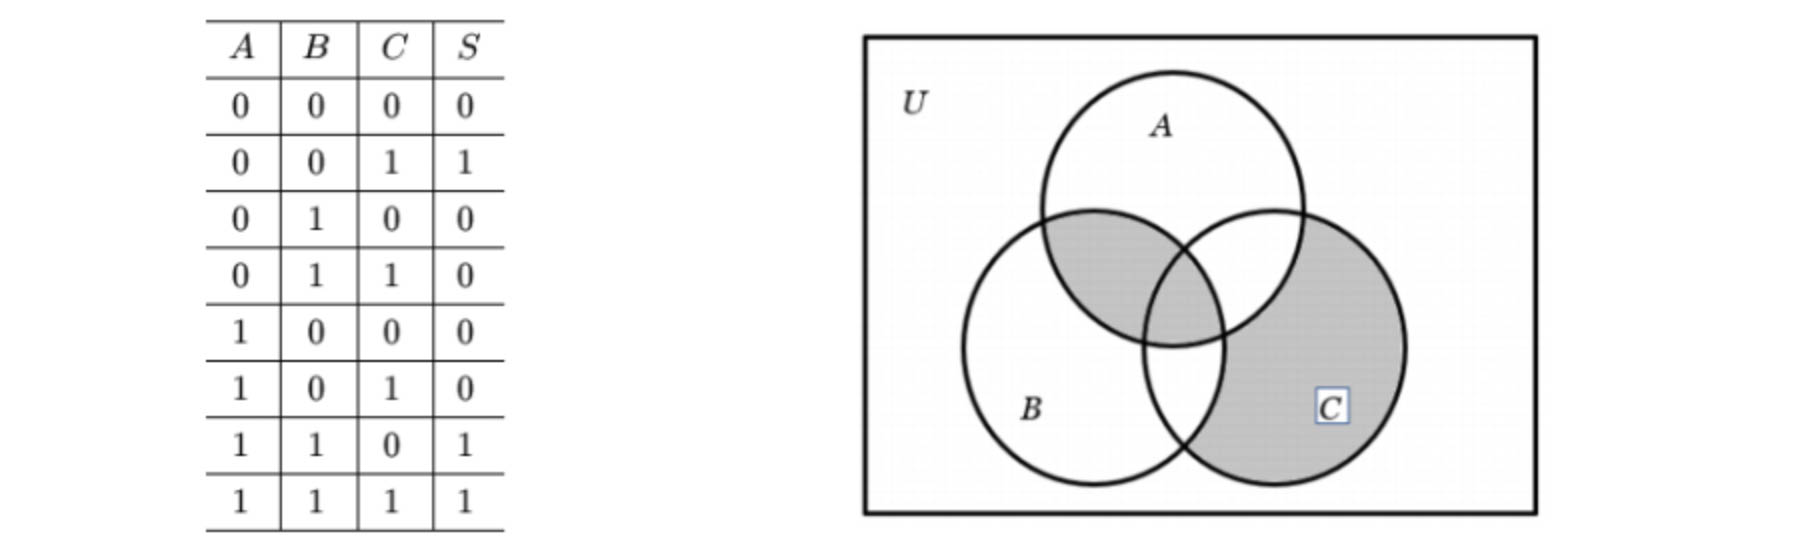
\includegraphics[width=0.9\textwidth]{5.16.jpg} % 插入图片
  \caption{测验题5.16用图}
\end{figure}


A. 对全集任意元素 $x$, 若 $x \in A$ 且 $x \in B$ 且 $x \in C$, 则 $x \in S$

B. 对全集任意元素 $x$, 若 $x \notin A$ 且 $x \in B$ 且 $x \in C$, 则 $x \in S$

C. 对全集任意元素 $x$, 若 $x \notin A$ 且 $x \notin B$ 且 $x \in C$, 则 $x \in S$

D. 上面右边给出的图是这个成员关系表所描述集合 $S$ 的文氏图

\textcolor{red}{答案:ACD}

\subsubsection{测验题5.17}
对于下面的成员关系表(见\textit{测验题5.17用图}),下面哪些说法是正确的?

\begin{figure}[htbp]
  \centering
  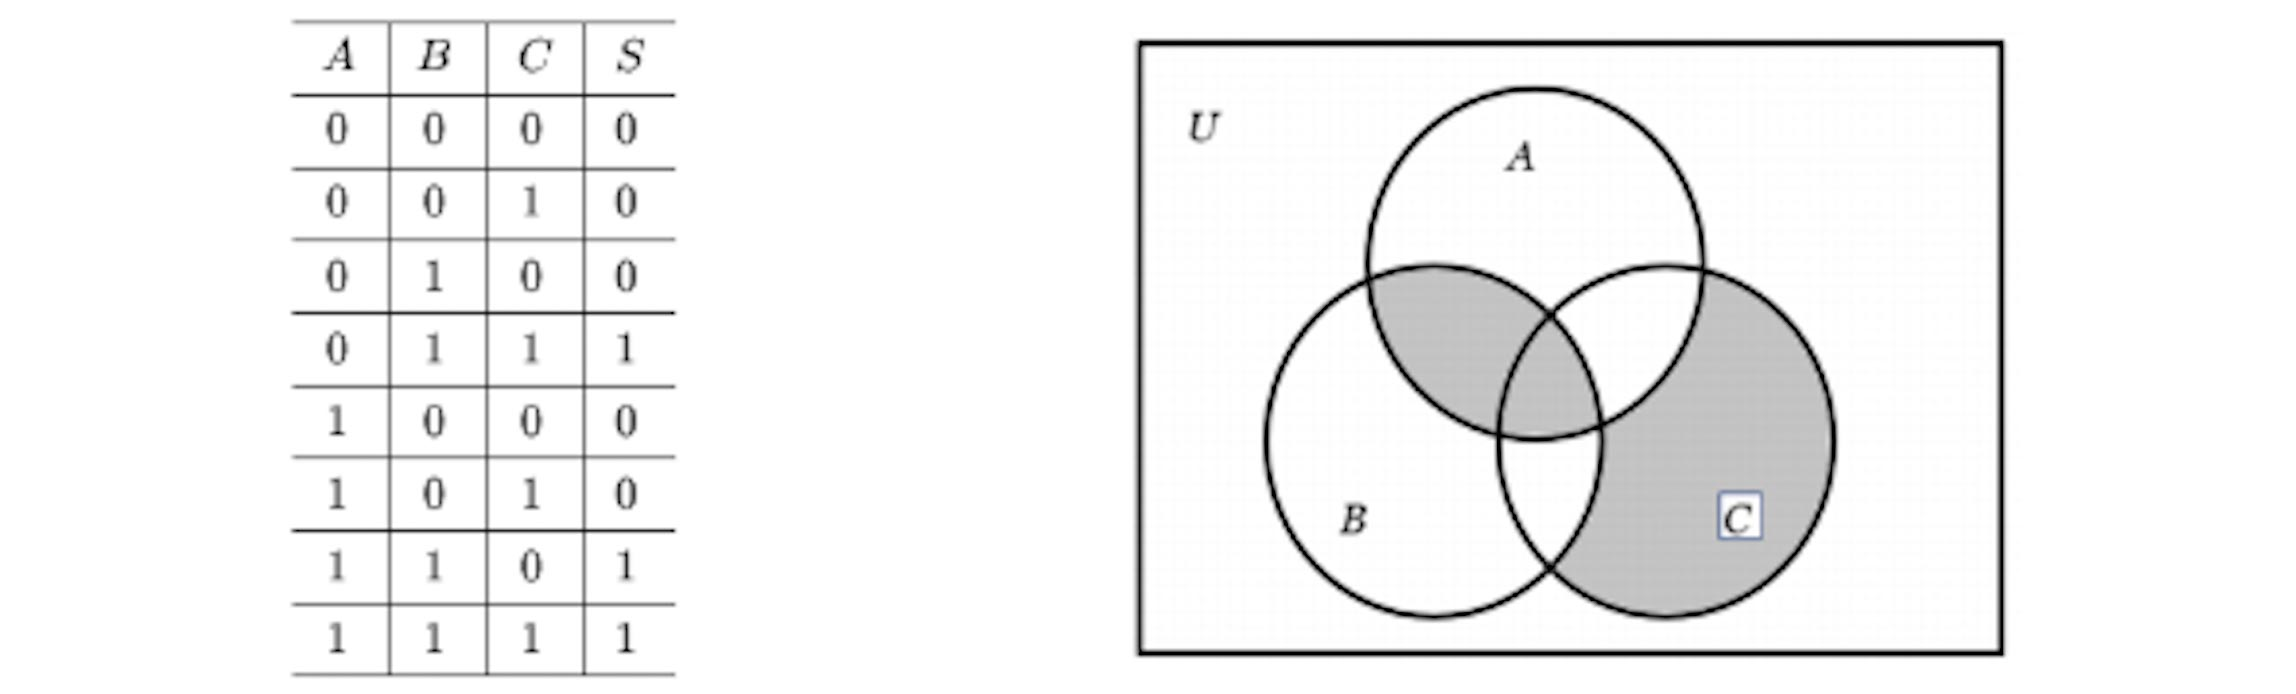
\includegraphics[width=0.9\textwidth]{5.17.jpg} % 插入图片
  \caption{测验题5.17用图}
\end{figure}

A. 对全集任意元素 $x$, 若 $x \in A$ 且 $x \in B$, 则 $x \in S$

B. 对全集任意元素 $x$, 若 $x \notin A$ 且 $x \in B$, 则 $x \in S$

C. 对全集任意元素 $x$, 若 $x \notin A$ 且 $x \notin B$, 则 $x \notin S$

D. 上面右边给出的图是这个成员关系表所描述集合 $S$ 的文氏图

\textcolor{red}{答案:AC}


\subsubsection{测验题5.18}
对于下面的成员关系表(见\textit{测验题5.18用图}),下面哪些说法是正确的?

\begin{figure}[htbp]
  \centering
  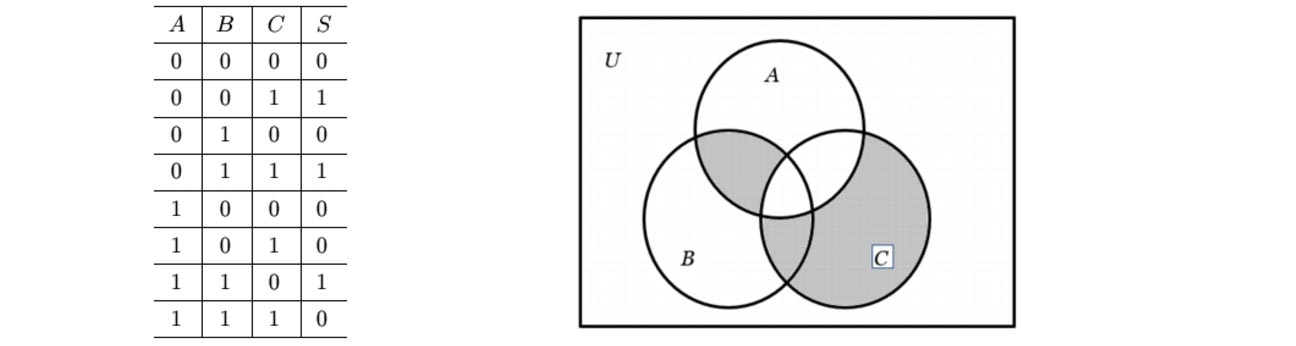
\includegraphics[width=1\textwidth]{5.18.jpg} % 插入图片
  \caption{测验题5.18用图}
\end{figure}

A. 对全集任意元素 $x$, 若 $x \in A$ 且 $x \in B$, 则 $x \in S$

B. 对全集任意元素 $x$, 若 $x \notin A$ 且 $x \in C$, 则 $x \in S$

C. 对全集任意元素 $x$, 若 $x \notin A$ 且 $x \notin B$, 则 $x \notin S$

D. 上面右边给出的图是这个成员关系表所描述集合 $S$ 的文氏图



\textcolor{red}{答案:BD}

\subsubsection{测验题5.21}

设全集 $U=\{x \in \mathbb{N} \mid 0 \leq x \leq 9\}$, 集合 $A=\{0,1,6,7,8,9\}, B=\{2,4,6,8\}, C=\{0,4,8,9\}$. 下面哪些命题是正确的?

A. $\{2,6\} \subseteq(A \cup B)-C$

B. $\{2,6\} \subseteq(A \cap B)-C$

C. $\{2,6\} \subseteq A \cup(B-C)$

D. $\{2,6\} \subseteq A \cap(B-C)$

\textcolor{red}{答案:AC}

\subsubsection{测验题5.22}

设全集 $U=\{x \in \mathbb{N} \mid 0 \leq x \leq 9\}$, 
集合 $A=\{0,1,6,7,8,9\}, B=\{2,4,6,8\}, C=\{0,4,8,9\}$ 。下面哪些命题是正确的?

A. $\{1,6,7\} \subseteq A \cap(\overline{B \cup C})$

B. $\{1,6,7\} \subseteq A \cap(\overline{B \cap C})$

C. $\{2,3,5\} \subseteq \bar{A}-(B \cup C)$

D. $\{2,3,5\} \subseteq \bar{A}-(B \cap C)$

\textcolor{red}{答案:BD}

\subsubsection{测验题5.23}
设全集 $U$ 是自然数集 $\mathbb{N}$, 定义集合 $A=\{3 k+2 \mid k \in \mathbb{N}\}, B=\{4 k+2 \mid k \in \mathbb{N}\}$ 。下面哪些命题是正确的?

A. 对任意自然数 $k, 12 k+5 \in A \cap B$

B. 对任意自然数 $k, 12 k+5 \in A \cup B$

C. 对任意自然数 $k, 12 k+5 \in A-B$

D. 对任意自然数 $k, 12 k+5 \in \bar{B}$

\textcolor{red}{答案:BCD}

\subsubsection{测验题5.24}

设全集 $U$ 是自然数集 $\mathbb{N}$, 定义集合 $A=\{3 k+2 \mid k \in \mathbb{N}\}, B=\{4 k+1 \mid k \in \mathbb{N}\}$ 。下面哪些命题是正确的?

A. 对任意自然数 $k, 12 k+5 \in A \cap B$

B. 对任意自然数 $k, 12 k+5 \in A \cup B$

C. 对任意自然数 $k, 12 k+5 \in A-B$

D. 对任意自然数 $k, 12 k+5 \in \bar{B}$

\textcolor{red}{答案:AB}

\subsubsection{测验题5.25}
设全集 $U$ 是自然数集 $\mathbb{N}$, 定义集合 $A=\{3 k+1 \mid k \in \mathbb{N}\}, B=\{4 k+2 \mid k \in \mathbb{N}\}$. 下面哪些命题
是正确的?

A. 对任意自然数 $k, 12 k+10 \in A \cap B$

B. 对任意自然数 $k, 12 k+10 \in A \cup B$

C. 对任意自然数 $k, 12 k+10 \in A-B$

D. 对任意自然数 $k, 12 k+10 \in \bar{A}$

\textcolor{red}{答案:AB}

\subsubsection{测验题5.26}

设全集 $U$ 是正整数集 $\mathbb{Z}^{+}$, 对任意正整数 $n$, 定义集合 $A_n$ 是 $n$ 的所有正因子构成的集合, 对于集合族 $\mathcal{A}=\left\{A_{12}, A_{18}, A_{24}, A_{36}\right\}$, 下面哪些命题是正确的?

A. $\bigcap \mathcal{A}=\{1,2,3\}$

B. $\{1,2,3\} \subseteq \bigcap \mathcal{A}$

C. $\bigcup \mathcal{A}=\{1,2,3,4,6,12\}$

D. $\{1,2,3,4,6,12\} \subseteq \bigcup \mathcal{A}$

\textcolor{red}{答案:BD}

\subsubsection{测验题5.27}

设全集 $U$ 是正整数集 $\mathbb{Z}^{+}$, 对任意正整数 $n$, 定义集合 $A_n$ 是 $n$ 的所有正因子构成的集合, 对于集合族 $\mathcal{A}=\left\{A_{12}, A_{18}, A_{24}, A_{36}\right\}$, 下面哪些命题是正确的?

A. 对任意正整数 $k$, 若 $k \in \bigcap \mathcal{A}$, 则 $k$ 是 12 的正因子

B. 对任意正整数 $k$, 若 $k \in \bigcup \mathcal{A}$, 则 $k$ 是 12 的正因子

C. 对任意正整数 $k$ ,只要 $k$ 是 12 的正因子,则 $k \in \bigcap \mathcal{A}$

D. 对任意自然数 $k$, 只要 $k$ 是 12 的正因子, 则 $k \in \bigcup \mathcal{A}$

\textcolor{red}{答案:AD}


\subsubsection{测验题5.29}
下面哪些命题是正确的?

A. 对任意集合 $A, B, A \cap B=A$ 当且仅当 $A \subseteq B$

B. 对任意集合 $A, B, A \cap B=A$ 当且仅当 $B \subseteq A$

C. 对任意集合 $A, B, C, A \cap B \subseteq C$ 当且仅当 $A \subseteq C$ 且 $B \subseteq C$

D. 对任意集合 $A, B, C, C \subseteq A \cap B$ 当且仅当 $C \subseteq A$ 且 $C \subseteq B$

\textcolor{red}{答案:AD}

\subsubsection{测验题5.30}
A. 对任意集合 $A, B, A \cup B=A$ 当且仅当 $A \subseteq B$

B. 
对任意集合 $A, B, A \cup B=A$ 当且仅当 $B \subseteq A$

C. 
对任意集合 $A, B, C, A \cup B \subseteq C$ 当且仅当 $A \subseteq C$ 且 $B \subseteq C$

D. 
对任意集合 $A, B, C, C \subseteq A \cup B$ 当且仅当 $C \subseteq A$ 且 $C \subseteq B$

\textcolor{red}{答案:BC}

\subsubsection{测验题5.31}

下面哪些命题是正确的?

A. 对任意集合 $A, B, C, A \cap B \subseteq C$ 当且仅当 $A \subseteq C$ 且 $B \subseteq C$

B. 对任意集合 $A, B, C, A \cup B \subseteq C$ 当且仅当 $A \subseteq C$ 且 $B \subseteq C$

C. 对任意集合 $A, B, C, C \subseteq A \cup B$ 当且仅当 $C \subseteq A$ 且 $C \subseteq B$

D. 对任意集合 $A, B, C, C \subseteq A \cap B$ 当且仅当 $C \subseteq A$ 且 $C \subseteq B$

\textcolor{red}{答案:BD}

\subsubsection{测验题5.32}

A. 
对任意集合 $A, B, A \subseteq B$ 当且仅当 $A-B=\varnothing$

B. 
对任意集合 $A, B, A \subseteq B$ 当且仅当 $B-A=\varnothing$

C. 
对任意集合 $A, B, A \subseteq B$ 当且仅当 $\bar{A} \subseteq \bar{B}$

D. 
对任意集合 $A, B, A \subseteq B$ 当且仅当 $\bar{B} \subseteq \bar{A}$

\textcolor{red}{答案:AD}

\subsubsection{测验题5.33}

下面哪些命题是正确的?

A. 对任意集合 $A, B, \bar{A} \subseteq \overline{A \cap B}$

B. 对任意集合 $A, B, \bar{A} \subseteq \overline{A \cup B}$

C. 对任意集合 $A, B, \bar{A} \subseteq \overline{A-B}$

D. 对任意集合 $A, B, \bar{A} \subseteq \overline{B-A}$

\textcolor{red}{答案:AC}

\subsubsection{测验题5.34}
下面哪些命题是正确的?

A. 
对任意集合 $A, B, A-B=A \cup \bar{B}$

B. 对任意集合 $A, B, A-B=\bar{A} \cup B$

C. 对任意集合 $A, B, A-B=A \cap \bar{B}$

D. 对任意集合 $A, B, A-B=\bar{A} \cap B$

\textcolor{red}{答案:C}


\subsubsection{测验题5.35}
下面哪些命题是正确的?

A. 对任意集合 $A, B, A \subseteq B$ 当且仅当 $A=A \cup B$

B. 对任意集合 $A, B, A \subseteq B$ 当且仅当 $A=A \cap B$

C. 对任意集合 $A, B, A \subseteq B$ 当且仅当 $A=A-B$

D. 对任意集合 $A, B, A \subseteq B$ 当且仅当 $\varnothing=A-B$

\textcolor{red}{答案:BD}

\subsubsection{测验题5.37}
A. 
空集 $\varnothing$ 的幂集 $\wp(\varnothing)$ 等于 $\varnothing$

B. 
集合 $\{\varnothing\}$ 的幂集 $\wp(\{\varnothing\})$ 等于 $\{\varnothing\}$

C. 
集合 $\{\varnothing\}$ 是幂集 $\wp(\varnothing)$ 的一个元素

D. 
集合 $\{\varnothing\}$ 是幂集 $\wp(\{\varnothing\})$ 的一个元素

\textcolor{red}{答案:D}

\subsubsection{测验题5.38}
A. 
集合 $\{\{\varnothing\}\}$ 是空集 $\varnothing$ 的幂集 $\varnothing(\varnothing)$ 的子集, 即有 $\{\{\varnothing\}\} \subseteq \wp(\varnothing)$

B. 
集合 $\{\{\varnothing\}\}$ 是空集 $\varnothing$ 的幂集 $\varnothing(\varnothing)$ 的元素, 即有 $\{\{\varnothing\}\} \in \wp(\varnothing)$

C. 
集合 $\{\{\varnothing\}\}$ 是集合 $\{\varnothing\}$ 的幂集 $\varphi(\{\varnothing\})$ 的子集, 即有 $\{\{\varnothing\}\} \subseteq \wp(\{\varnothing\})$

D. 
集合 $\{\{\varnothing\}\}$ 是集合 $p(\{\varnothing\})$ 的幂集 $\rho(\rho(\{\varnothing\})$ )的元素,即有 $\{\{\varnothing\}\} \in \wp(\wp(\{\varnothing\}))$

\textcolor{red}{答案:CD}

\subsubsection{测验题5.40}
对任意集合 $A, B, C$, 下面哪些命题是正确的?

A. $ A \cup B=A \cup C$ 蕴涵 $B=C$

B. $A \cap B=A \cap C$ 蕴涵 $B=C$

C. $A \cup B=A \cup C$ 且 $\bar{A} \cup B=\bar{A} \cup C$ 蕴涵 $B=C$

D. $A \cap B=A \cap C$ 且 $\bar{A} \cap B=\bar{A} \cap C$ 蕴涵 $B=C$

\textcolor{red}{答案:CD}


\subsubsection{测验题5.41}
下面的集合等式演算中 (1),(2)使用的集合基本等式分别是:
\begin{figure}[htbp]
    \centering
    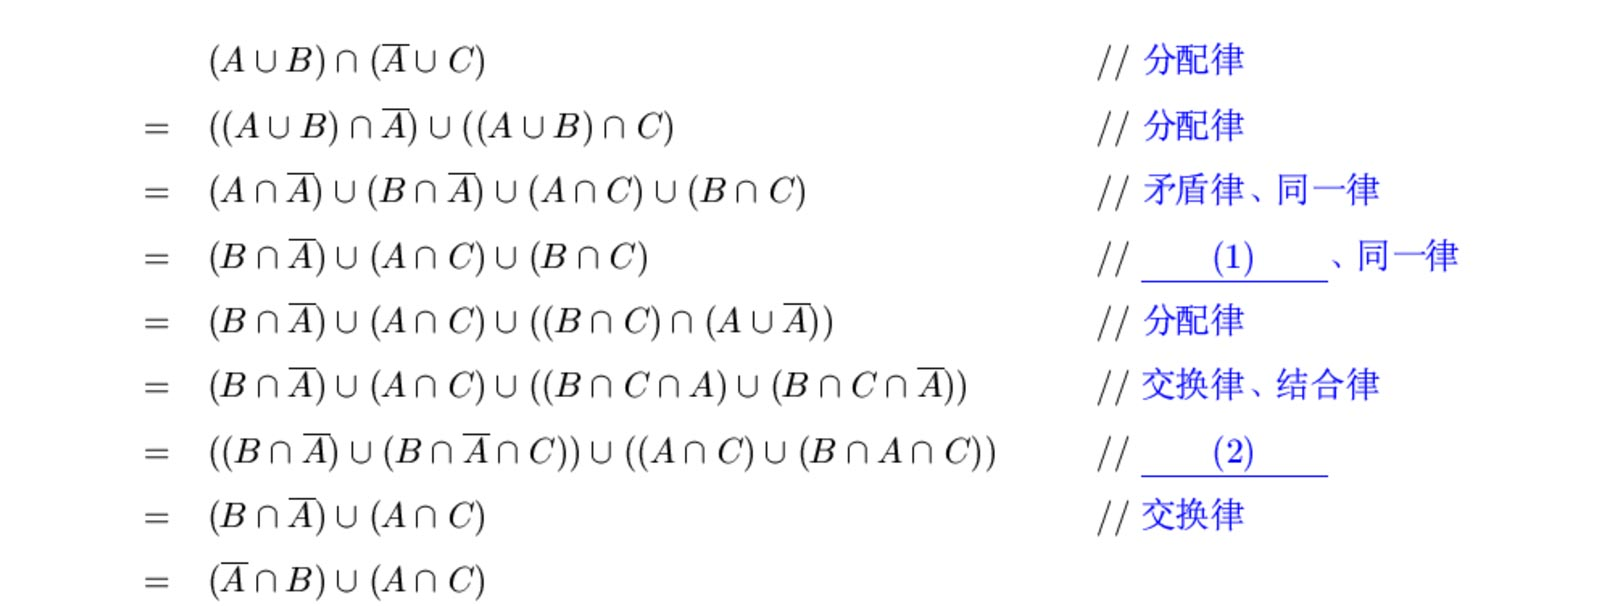
\includegraphics[width=1\textwidth]{5.41.jpg} % 插入图片
    \caption{测验题5.41用图}
\end{figure}

\textcolor{red}{答案:(1)排中律 (2)吸收律}

\subsubsection{测验题5.42}

\begin{figure}[htbp]
  \centering
  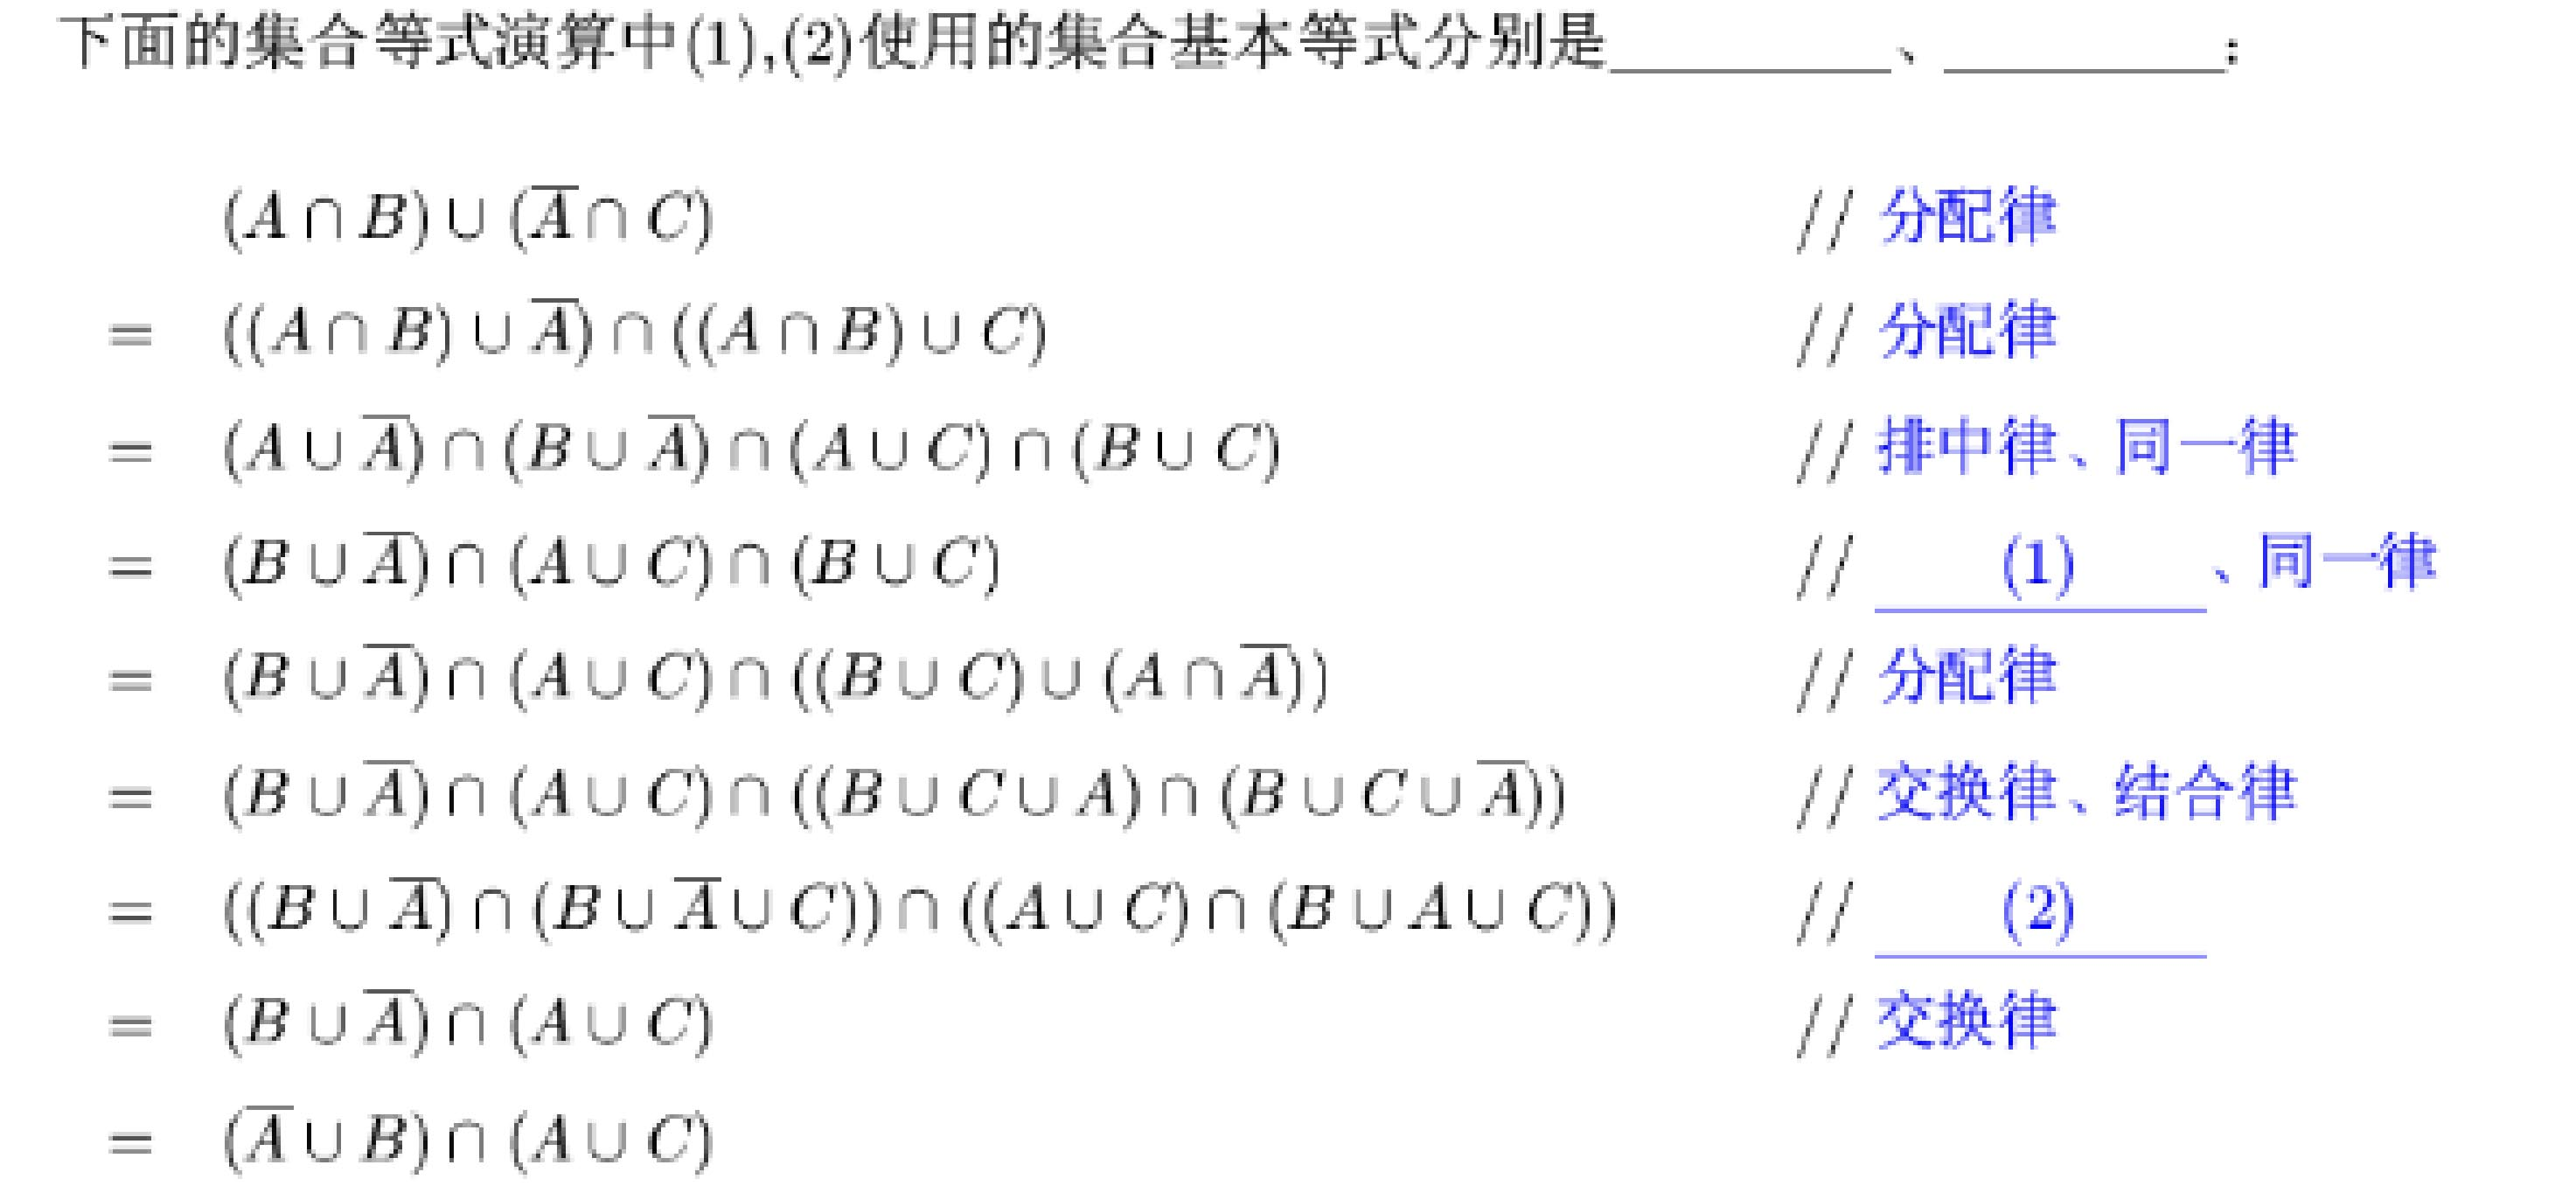
\includegraphics[width=1\textwidth]{5.42.jpg} % 插入图片
  \caption{测验题5.42用图}
\end{figure}
\textcolor{red}
{
  答案:(1)矛盾律
  (2)吸收律
}


\subsubsection{测验题5.43}
\begin{figure}[htbp]
  \centering
  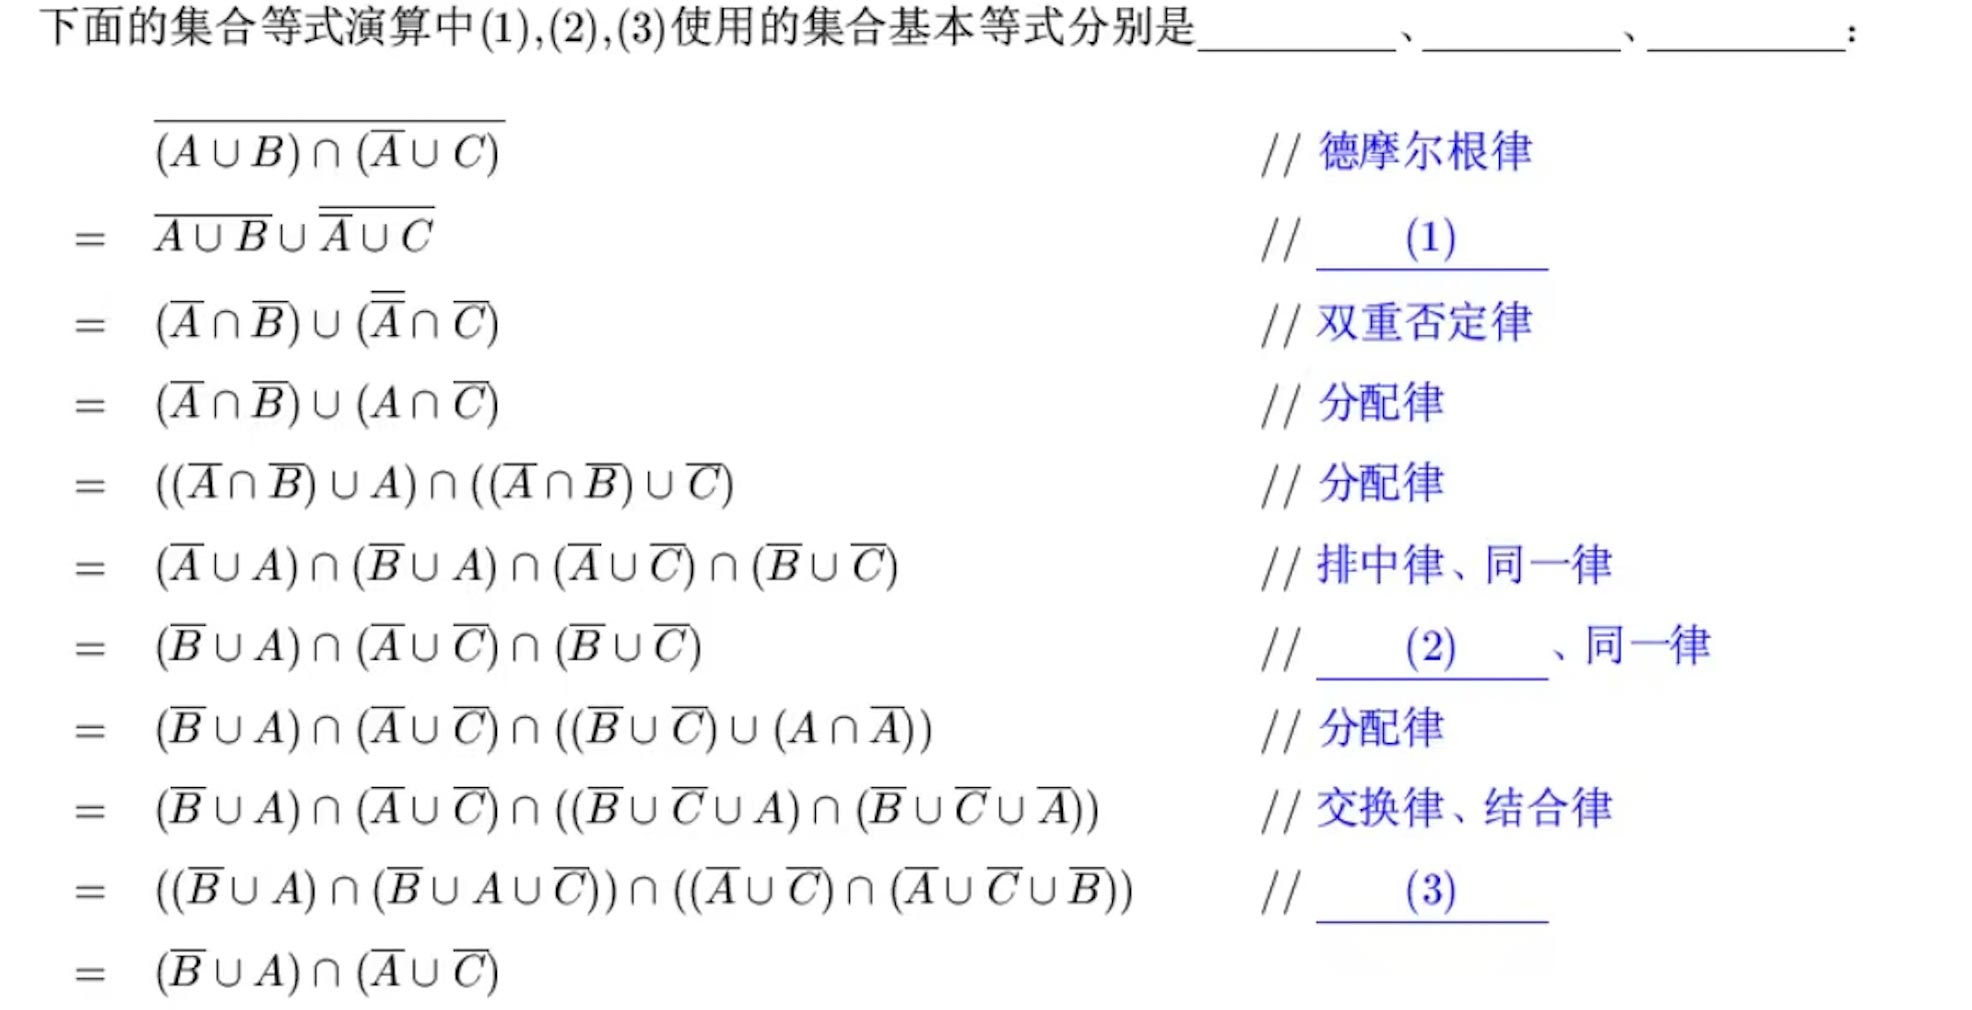
\includegraphics[width=1\textwidth]{5.43.jpg} % 插入图片
  \caption{测验题5.43用图}
\end{figure}
\textcolor{red}
{
  答案:(1)徳摩尔根律;德摩根律
  (2)矛盾律
  (3)吸收律
}

\subsubsection{测验题5.44}
\begin{figure}[htbp]
    \centering
    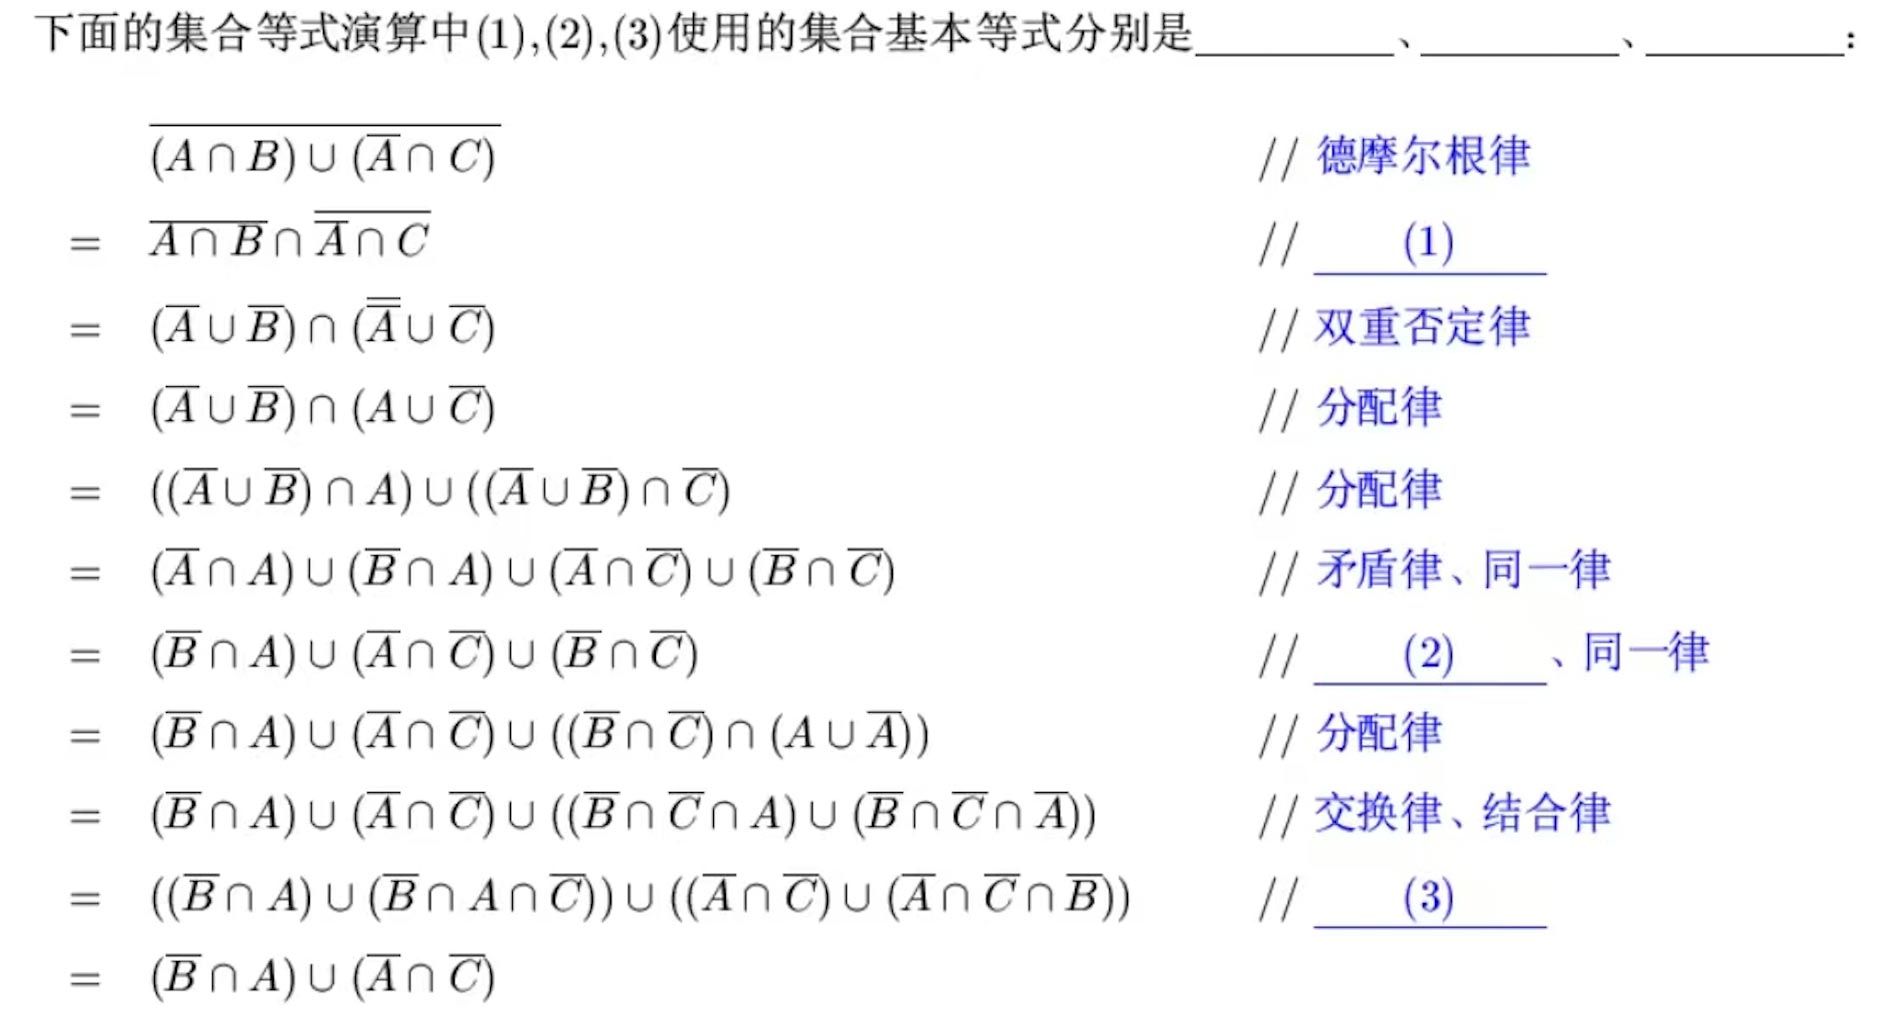
\includegraphics[width=1\textwidth]{5.44.jpg} % 插入图片
    \caption{测验题5.44用图}
\end{figure}

\textcolor{red}
{
  答案:(1)徳摩尔根律;德摩根律
  (2)排中律 
  (3)吸收律
}

\subsubsection{测验题5.46}
设 $A, B$ 是任意集合, 且已知对称差 $\oplus$ 定义为 $A \oplus B=(A \cup B)-(A \cap B)$. 下面哪一组的两个集合表达式给出的集合是相等的?

A. 集合 $(A-B) \cap A$ 和集合 $A \cap B$

B. 集合 $(A-B) \cup A$ 和集合 $A \cup B$

C. 集合 $(A \oplus B) \cap A$ 和集合 $A \cap B$

D. 集合 $(A \oplus B) \cup A$ 和集合 $A \cup B$

\textcolor{red}{答案:D}

% \clearpage

\subsubsection{测验题5.47}

设 $A, B$ 是任意集合, 且已知对称差 $\oplus$ 定义为 $A \oplus B=(A \cup B)-(A \cap B)$. 下面哪一组的两个集
合表达式给出的集合是相等的?

A. 集合 $\overline{A-B}$ 和集合 $\bar{A}-B$

B. 集合 $\overline{A-B}$ 和集合 $\bar{A}-\bar{B}$

C. 集合 $\overline{A \oplus B}$ 和集合 $\bar{A} \oplus B$

D. 集合 $\overline{A \oplus B}$ 和集合 $\bar{A} \oplus \bar{B}$

\textcolor{red}{答案:C}

\subsubsection{测验题5.48}
设A, B, C是任意集合, 下面哪一组的两个集合表达式给出的集合是不相等的?

A. 
集合 $(A-B)-C$ 和集合 $A-(B-C)$

B. 
集合 $(A-B)-C$ 和集合 $(A-C)-B$

C. 
集合 $(A-B)-C$ 和集合 $A-(B \cup C)$

D. 
集合 $(A-B)-C$ 和集合 $(A-C)-(B-C)$

\textcolor{red}{答案:A}

\subsubsection{测验题5.51}

设 $A, B, C$ 是任意集合, $(A-B) \cup(A-C)=\varnothing$ 的充分必要条件是?

A. $A=B=C$

B. $A=B \cap C$

C. $A \subseteq B \cap C$

D. $A \subseteq B \cup C$

\textcolor{red}{答案:C}

\subsubsection{测验题5.52}

设 $A, B, C$ 是任意集合, $(A-B) \cap(A-C)=A$ 的充分必要条件是?

A. $A \cap B=\varnothing$ 且 $A \cap C=\varnothing$

B. $A \cap B \cap C=\varnothing$

C. $A \cup B \cup C=\varnothing$

D. $\bar{A} \subseteq B \cup C$

\textcolor{red}{答案:A}

\subsubsection{测验题5.54}

设 $A, B$ 是任意集合, $(A-B) \cup(B-A)=A$ 的充分必要条件是?

A. $A \cup B=\varnothing$

B. $A=\varnothing$

C. $A \cap B=\varnothing$

D. $B=\varnothing$

\textcolor{red}{答案:D}

\subsubsection{测验题5.55}
设 $A, B$ 是任意集合, $(A-B) \cup(B-A)=A \cup B$ 的充分必要条件是?

A. $A \cup B=\varnothing$

B. $A=\varnothing$

C. $A \cap B=\varnothing$

D. $B=\varnothing$

\textcolor{red}{答案:C}

\subsubsection{测验题5.56}

设 $A, B, C$ 是任意集合, 下面哪个命题是正确的?

A. 集合 $A \subseteq B \cup C$, 当且仅当 $A \subseteq B$ 或 $A \subseteq C$

B. 集合 $A \subseteq B \cap C$, 当且仅当 $A \subseteq B$ 且 $A \subseteq C$

C. 集合 $B \cap C \subseteq A$, 当且仅当 $B \subseteq A$ 且 $C \subseteq A$

D. 集合 $B \cup C \subseteq A$, 当且仅当 $B \subseteq A$ 或 $C \subseteq A$

\textcolor{red}{答案:B}



\subsubsection{测验题5.57}

\textbf{如果你查找的不是这道题,请查看测验题6.57}

设$A, B, C, D$是任意集合,下面哪些命题不是正确的?

A. 集合 $A \subseteq C$ 且 $B \subseteq D$, 蕴涵 $A \cup B \subseteq C \cup D$

B. 集合 $A \subseteq C$ 且 $B \subseteq D$, 蕴涵 $A \cap B \subseteq C \cap D$

C. 集合 $A \subseteq C$ 且 $B \subseteq D$, 蕴涵 $A-B \subseteq C-D$

D. 集合 $A \subset C$ 且 $B \subset D$, 蕴涵 $A \cup B \subset C \cup D$


\textcolor{red}{答案:CD}

\textcolor{red}{解析:D选项反例:$A=\{1\},B=\{2\},C=D=\{1,2\}$.}

\subsubsection{测验题5.58}
设 $A, B, C, D$ 是任意集合, 下面哪些命题不是正确的?

A. 
集合 $A \subseteq C$ 且 $B \subseteq D$, 蕴涵 $A \cup B \subseteq C \cup D$

B. 
集合 $A \subset C$ 且 $B \subset D$, 蕴涵 $A \cap B \subset C \cap D$

C. 
集合 $A \subseteq C$ 且 $B \subseteq D$, 蕴涵 $A-B \subseteq C-D$

D. 
集合 $A \subseteq C$ 且 $B \subseteq D$. 蕴涵 $A-D \subseteq C-B$

\textcolor{red}{答案:BC}

\subsubsection{测验题5.59}

设 $A, B, C$ 是任意集合且 $A-B \subseteq C$, 证明 $A-C \subseteq B$. 下面的证明是否正确?

【证明】对任意元素 $x \in A-B$, 则 $x \in A$ 且 $x \notin B$, 而 $A-B \subseteq C$, 因此 $x \in C$, 因此 $x \notin A-C$,这表明当 $x \notin B$ 时有 $x \notin A-C$, 因此 $A-C \subseteq B$.

\textcolor{red}{答案:错}
\subsubsection{测验题5.60}
设 $A, B$ 是任意集合且 $A \subseteq B$, 证明 $\wp(A) \subseteq \wp(B)$, 下面的证明是否正确?

【证明】对任意 $x \in A$, 因此 $\{x\} \in \wp(A)$, 而由 $A \subseteq B$ 有 $x \in B$, 从而也有 $\{x\} \in \wp(B)$, 因此 $\wp(A) \subseteq \wp(B)$ 。

\textcolor{red}{答案:错}


\clearpage

\section{关系}

\subsubsection{测验题6.1}

设A, B, C是任意集合, 对于笛卡尔积, 下面哪个等式是正确的?

A. 
$
A \times B=B \times A
$

B. 
$
A \times \varnothing=\varnothing \times A
$

C. 
$
A \times(B \times C)=(A \times B) \times C
$

D. 
$
A \times(A \times A)=(A \times A) \times A
$

\textcolor{red}{答案:B}


\subsubsection{测验题6.2}
设A, B, C, D是任意集合, 对于笛卡尔积, 下面哪个等式是正确的?

A. 
$
(A \cup B) \times(C \cup D)=(A \times C) \cup(B \times D)
$

B. 
$
(A \cap B) \times(C \cap D)=(A \times C) \cap(B \times D)
$

C. 
$
(A-B) \times(C-D)=(A \times C)-(B \times D)
$

D. 
$
(A-B) \times C=(A \times C)-(B \times C)
$

\textcolor{red}{答案:D}

\subsubsection{测验题6.3}

设集合 $A=\{0,1,2,3\}, B=\{0,1,4,9\}$, 定义关系 $R=\{\langle a, b\rangle \in A \times B \mid \exists c \in \mathbb{N}(b=a c)\}$ 。对于关系 $R$ ,下面哪些命题是正确的?

A. 定义集合 $S=\{x \in A \mid \forall y \in B(\langle x, y\rangle \in R)\}$, 则 $S=\{1\}$

B. 关系R的元素总共有 9 个有序对。

C. 右边的图是 $R$ 的关系图。

D. 下面的矩阵 $R$ 的关系矩阵, 其中每行依次对应 $A$ 的元素 $0,1,2,3$, 而每列依次对应 $B$ 的元素 $0,1,4,9$ 。

\begin{figure}[htbp]
    \centering
    \begin{minipage}[t]{0.45\textwidth}
        \centering
        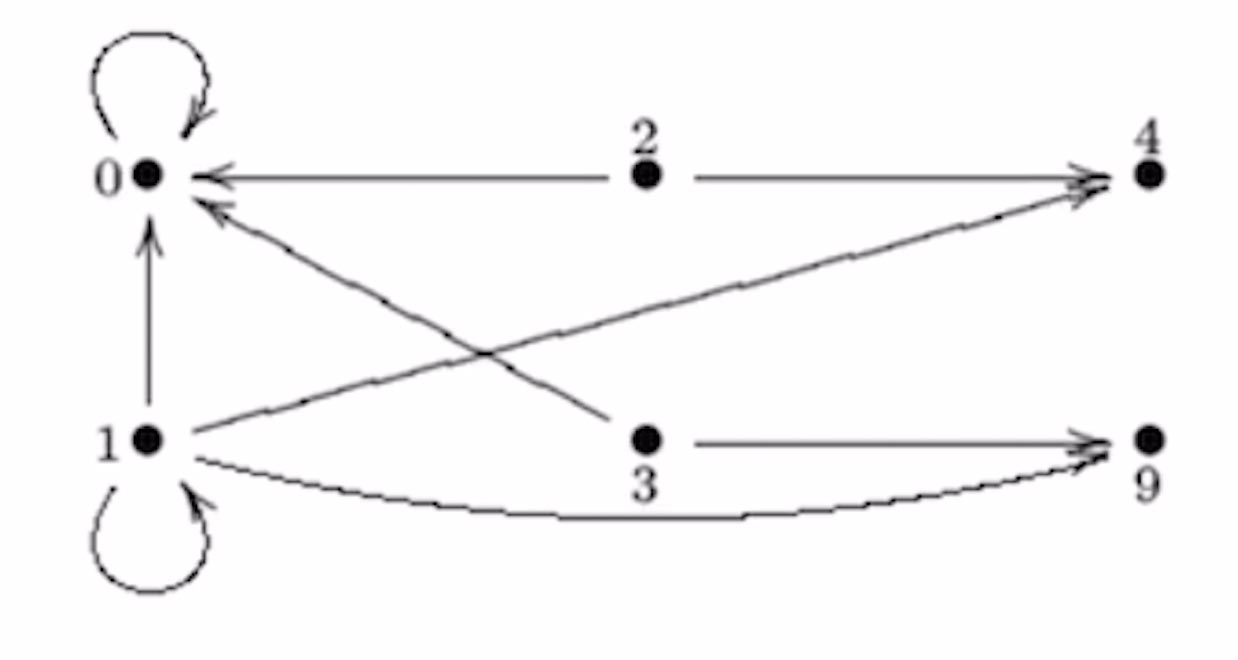
\includegraphics[width=1\textwidth]{6.3_1.jpg} % 插入图片
	      \vspace{-0.3cm}
        \caption{测验题6.3 C选项用图}
    \end{minipage}
	  \hspace{0.1\textwidth} % 调整这里的值来改变两张图片之间的间距
    \begin{minipage}[t]{0.23\textwidth}
        \centering
        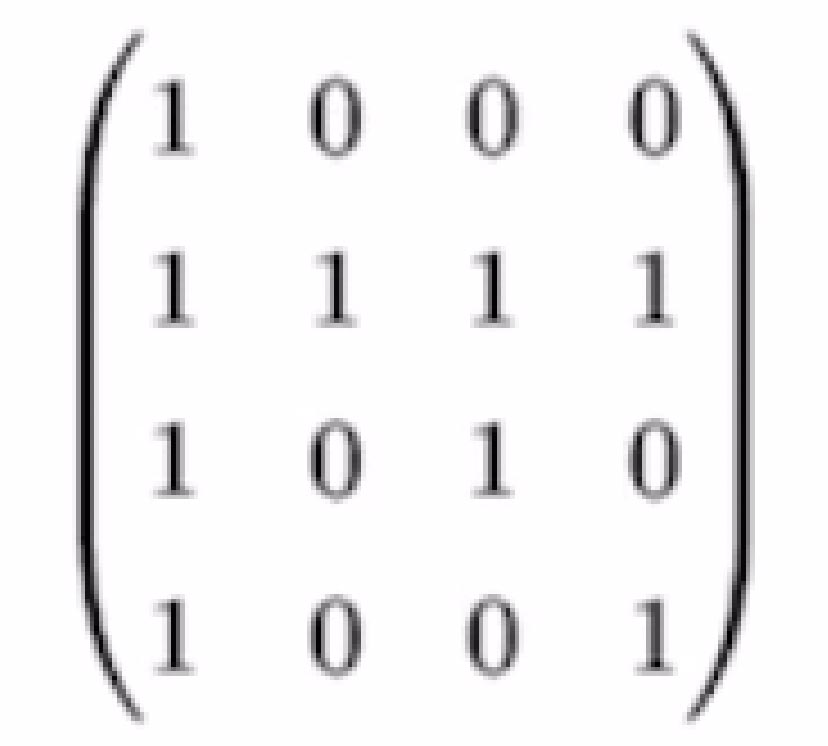
\includegraphics[width=1\textwidth]{6.3_2.jpg} % 插入图片
	      \vspace{-0.3cm}
        \caption{测验题6.3 D选项用图}
\end{minipage}
\end{figure}

\textcolor{red}{答案:ABD}


\subsubsection{测验题6.4}
设集合 $A=\{0,1,2,3,4,9\}$. 定义关系 $R=\{(a, b) \in A \times A \mid \exists c \in A(b=a c)\}$对于关系 $R$. 下面哪些命题是正确的?

A. 定义集合 $S=\{x \in A \mid \forall y \in B(\langle y, x\rangle \in R)\}$, 则 $S=\{0\}$

B. 
关系R的元素总共有9个有序对。

C. 
右边的图是 $R$ 的关系图。

D. 
下面的矩阵 $R$ 的关系矩阵。其中每行、每列依次对应 $A$ 的元素 $0,1,2,3,4,9$.

\begin{figure}[htbp]
    \centering
    \begin{minipage}[t]{0.45\textwidth}
        \centering
        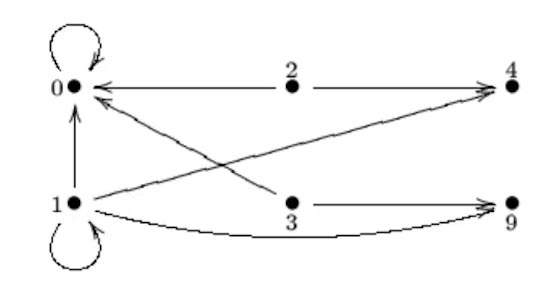
\includegraphics[width=1\textwidth]{6.4_1.jpg} % 插入图片
	      \vspace{-0.5cm}
        \caption{测验题6.4 C选项}
    \end{minipage}
	  \hspace{0.1\textwidth} % 调整这里的值来改变两张图片之间的间距
    \begin{minipage}[t]{0.3\textwidth}
        \centering
        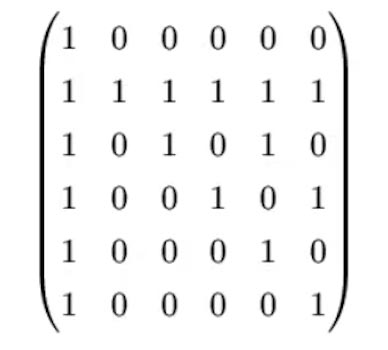
\includegraphics[width=1\textwidth]{6.4_2.jpg} % 插入图片
	      \vspace{-0.5cm}
        \caption{测验题6.4 D选项}
\end{minipage}
\end{figure}

\textcolor{red}{答案:AD}

\subsubsection{测验题6.5}

设集合 $A=\{0,1,2,3\}, B=\{0,1,4,9\}$, 定义关系 $R=\{\langle a, b\rangle \in A \times B \mid a \equiv b(\bmod 2)\}$ 。对于关系 $R$, 下面哪些命题是正确的?

A. 定义集合 $S=\{x \in A \mid\langle x, 4\rangle \in R)\}$, 则 $S=\{0,2,4\}$

B. 关系R的元素总共有 8 个有序对。

C. 右边的图是 $R$ 的关系图。

D. 下面的矩阵 $R$ 的关系矩阵, 其中每行依次对应 $A$ 的元素 $0,1,2,3$, 而每列依次对应 $B$ 的元素 $0,1,4,9$ 。


\begin{figure}[htbp]
    \centering
    \begin{minipage}[t]{0.45\textwidth}
        \centering
        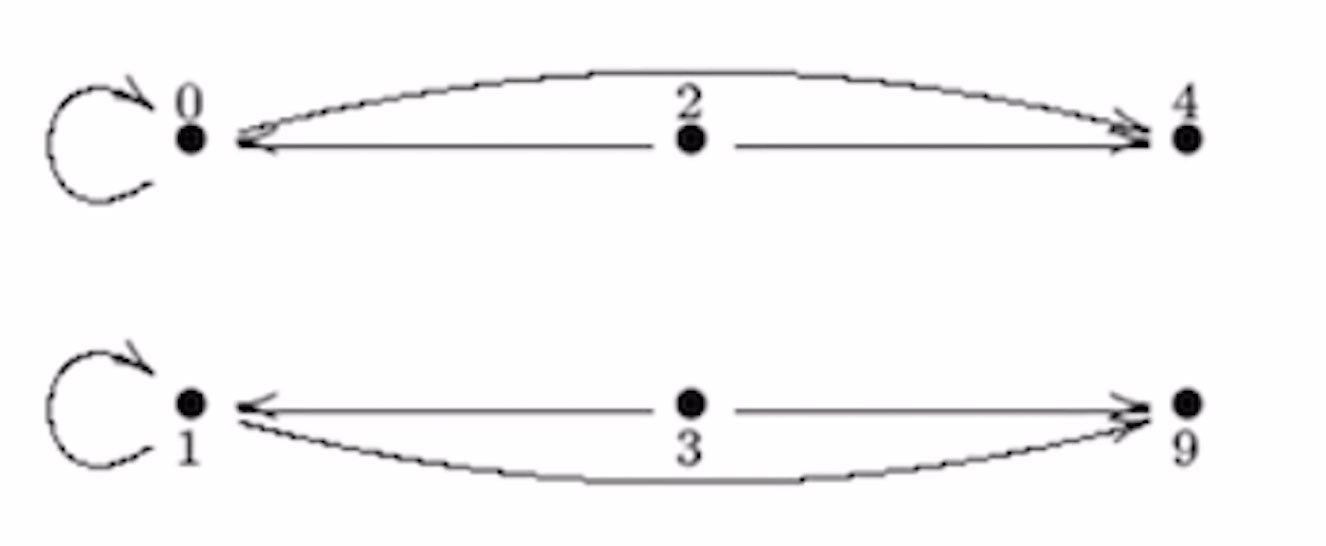
\includegraphics[width=1\textwidth]{6.5_1.jpg} % 插入图片
	      \vspace{-0.3cm}
        \caption{测验题6.5 C选项用图}
    \end{minipage}
    % \hfill
	  \hspace{0.1\textwidth} % 调整这里的值来改变两张图片之间的间距
    \begin{minipage}[t]{0.23\textwidth}
        \centering
        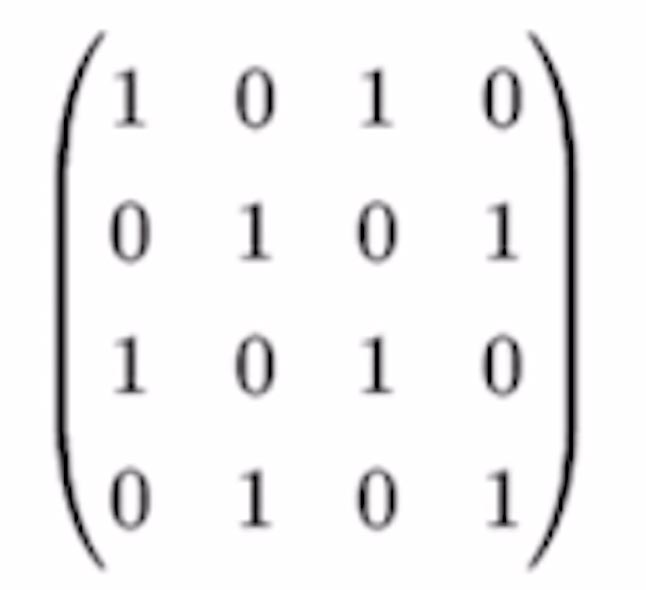
\includegraphics[width=1\textwidth]{6.5_2.jpg} % 插入图片
	      \vspace{-0.3cm}
        \caption{测验题6.5 D选项用图}
\end{minipage}
\end{figure}

\textcolor{red}{答案:BD}

\subsubsection{测验题6.6}

设集合 $A=\{0,1,2,3,4,9\}$, 定义关系 $R=\{\langle a, b\rangle \in A \times A \mid a \equiv b(\bmod 2)\}$ 。对于关系 $R$, 下面哪些是正确的?

A. 定义集合 $S=\{x \in A \mid\langle x, 4\rangle \in R)\}$, 则 $S=\{0,2,4\}$

B. 关系R的元素总共有 8 个有序对。

C. 右边的图是 $R$ 的关系图。

D. 下面的矩阵 $R$ 的关系矩阵, 其中每行、每列依次对应 $A$ 的元素 $0,1,2,3,4,9$ 。


\begin{figure}[htbp]
    \centering
    \begin{minipage}[t]{0.45\textwidth}
        \centering
        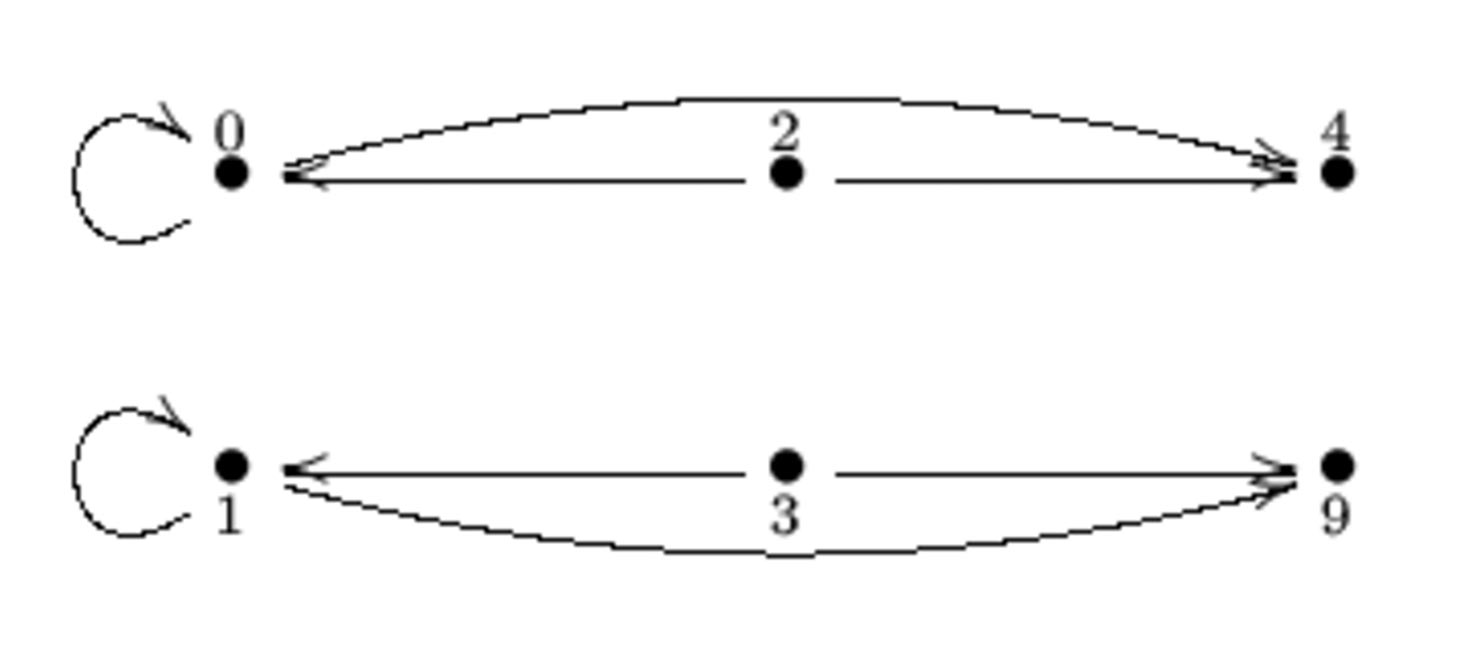
\includegraphics[width=1\textwidth]{6.6_1.jpg} % 插入图片
	      \vspace{-0.3cm}
        \caption{测验题6.6 C选项用图}
    \end{minipage}
    \hfill
	%   \hspace{0.1\textwidth} % 调整这里的值来改变两张图片之间的间距
    \begin{minipage}[t]{0.23\textwidth}
        \centering
        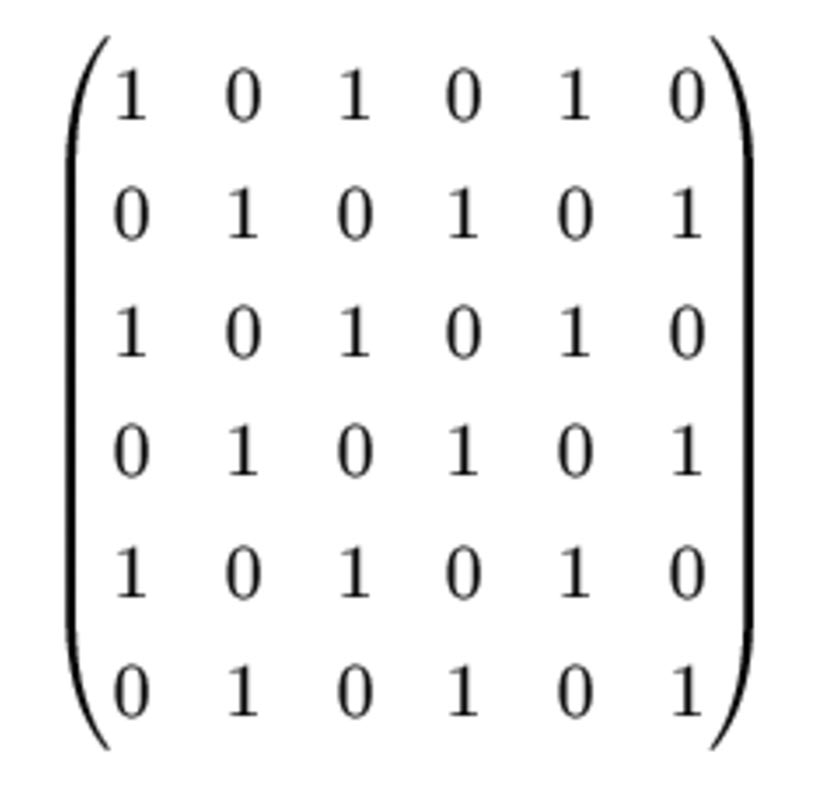
\includegraphics[width=1\textwidth]{6.6_2.jpg} % 插入图片
	      \vspace{-0.3cm}
        \caption{测验题6.6 D选项用图}
\end{minipage}
\end{figure}

\textcolor{red}{答案:AD}



\subsubsection{测验题6.7}

设集合 $A=\{1,2,3,4,5\}$, 关系 $R=\{(3,2\rangle,\langle 3,3\rangle,\langle 1,1\rangle,\langle 3,1\rangle,\langle 1,4\rangle,\langle 3,5\rangle\}, S=\{\langle 2,2\rangle,\langle 4,5\rangle,\langle 3,3\rangle,\langle 5,5\rangle\}$.
下面哪些关系运算的结果是正确的?

A. $R^{-1}=\{\langle 2,3\rangle,\langle 1,3\rangle,\langle 4,1\rangle,\langle 5,3\rangle\}$

B. $S \circ R=\{\langle 3,2\rangle,\langle 3,3\rangle,\langle 3,1\rangle,\langle 3,5\rangle\}$

C. $R \circ S=\{\langle 3,2\rangle,\langle 3,3\rangle,\langle 1,5\rangle,\langle 3,5\rangle\}$

D. 
$R^{-1} \circ S^{-1}=\{\langle 2,3\rangle,\langle 5,1\rangle,\langle 3,3\rangle,\langle 5,3\rangle\}$

\textcolor{red}{答案:D}


\subsubsection{测验题6.8}

设集合 $A=\{1,2,3,4,5\}$, 关系 $R=\{(3,2),\langle 3,3\rangle,\langle 1,1),(3,1\rangle,\langle 1,4\rangle\}, S=\{(2,2\rangle,\langle 4,5),(3,3\rangle,\langle 5,5\rangle,(4,1\rangle\}$.下面哪些关系运算的结果是正确的?

A. $S^{-1}=\{\langle 2,2\rangle,\langle 5,4\rangle,\langle 3,3\rangle,\langle 5,5\rangle,\langle 1,4\rangle\}$

B. ${S \circ R}=\{\langle 2,3\rangle,\langle 5,1\rangle,\langle 3,3\rangle,\langle 1,1\rangle\}$

C. ${R \circ S}=\{\langle 3,2\rangle,\langle 3,3\rangle,\langle 3,1\rangle,\langle 4,1\rangle,\langle 4,4\rangle\}$

D. $R^{-1} \circ S^{-1}=\{\langle 2,3\rangle,\langle 3,3\rangle,\langle 1,4\rangle,\langle 1,3\rangle,\langle 4,4\rangle\}$

\textcolor{red}{答案:AC}

\subsubsection{测验题6.9}

设集合 $A=\{1,2,3,4,5\}$ ,关系 $R=\{\langle 5,5\rangle,\langle 5,3\rangle,\langle 4,5\rangle,\langle 1,3\rangle,\langle 2,4\rangle\}, S=\{\langle 1,1\rangle,\langle 1,3\rangle,\langle 5,4\rangle,\langle 2,3\rangle,, 4,3\rangle\}$.
下面哪些关系运算的结果是正确的?

A. $ R^{-1}=\{\langle 3,5\rangle,\langle 5,4\rangle,\langle 3,1\rangle,\langle 4,2\rangle\} $

B. $S \circ R=\{\langle 5,4\rangle,\langle 4,4\rangle,\langle 2,3\rangle\} $

C. $ R \circ S=\{\langle 1,3\rangle,\langle 5,5\rangle\} $

D. $ S^{-1} \circ R^{-1}=\{\langle 4,5\rangle,\langle 4,4\rangle,\langle 3,2\rangle\}$

\textcolor{red}{答案:BC}


\subsubsection{测验题6.10}

设集合 $A=\{1,2,3,4,5\}$ ,关系 $R=\{\langle 5,4\rangle,\langle 5,3\rangle,\langle 4,2\rangle,\langle 1,3\rangle,\langle 2,4\rangle\}, S=\{\langle 1,1\rangle,\langle 1,3\rangle,\langle 5,2\rangle,\langle 2,3\rangle,\langle 4,2\rangle\}$.
下面哪些关系运算的结果是正确的?

A. $S^{-1}=\{\langle 3,1\rangle,\langle 2,5\rangle,\langle 3,2\rangle,\langle 2,4\rangle\}$

B. $R \circ S=\{\langle 1,3\rangle,\langle 5,4\rangle,\langle 4,4\rangle\}$

C. $ S \circ R=\{\langle 3,4\rangle,\langle 2,5\rangle,\langle 2,2\rangle\}$

D. $ S^{-1} \circ R^{-1}=\{\langle 3,1\rangle,\langle 4,5\rangle,\langle 4,4\rangle\}$

\textcolor{red}{答案:BD}



\subsubsection{测验题6.11}

设 $A=\{1,2,3,4,5\}$, 关系 $R=\{(4,5),(3,3),(1,4),(1,3),\langle 2,4),(5,4)\}, S=\{(1,4),(5,1),(5,4),(2,5),\langle 2,3)\}$,下面哪些使用关系矩阵表示的关系运算结果是正确的?

A. 关系 $R^{-1}$ 的关系矩阵是 $M_{R^{-1}}=\left[\begin{array}{lllll}0 & 0 & 0 & 0 & 0 \\ 0 & 0 & 0 & 0 & 0 \\ 1 & 0 & 0 & 0 & 0 \\ 1 & 1 & 0 & 0 & 1 \\ 0 & 0 & 0 & 1 & 0\end{array}\right]$

B. 关系 $R \circ S$ 的关系矩阵是 $M_{R \circ S}=\left[\begin{array}{ccccc}0 & 0 & 0 & 0 & 0 \\ 0 & 0 & 0 & 0 & 0 \\ 0 & 0 & 0 & 0 & 0 \\ 1 & 0 & 0 & 1 & 0 \\ 0 & 0 & 0 & 0 & 0\end{array}\right]$

C. 关系 $R^{-1} \circ S^{-1}$ 的关系矩阵是 $M_{R^{-1} \circ S^{-1}}=\left[\begin{array}{ccccc}0 & 0 & 0 & 1 & 0 \\ 0 & 0 & 0 & 0 & 0 \\ 0 & 0 & 0 & 0 & 0 \\ 0 & 0 & 0 & 1 & 0 \\ 0 & 0 & 0 & 0 & 0\end{array}\right]$

D. 关系 $S^{-1} \circ R^{-1}$ 的关系矩阵是 $M_{S^{-1} \circ R^{-1}}=\left[\begin{array}{ccccc}0 & 0 & 0 & 0 & 0 \\ 0 & 0 & 0 & 0 & 0 \\ 0 & 1 & 0 & 0 & 1 \\ 0 & 1 & 0 & 0 & 1 \\ 1 & 0 & 0 & 0 & 1\end{array}\right]$

\textcolor{red}{答案:CD}

\subsubsection{测验题6.12}

设 $A=\{1,2,3,4,5\}$. 关系 $R=\{(4,5\rangle,\langle 3,3\rangle,(2,4),(2,5),(5,4)\}, S=\{(1,4),(5,2),\langle 5,4),(2,5\rangle,(2,4)\}$.
下面哪些使用关系矩阵表示的关系运算结果是正确的?

A. 关系 $S^{-1}$ 的关系矩阵是 $M_{S^{-1}}=\left[\begin{array}{ccccc}0 & 0 & 0 & 0 & 0 \\ 0 & 0 & 0 & 0 & 1 \\ 0 & 0 & 0 & 0 & 0 \\ 1 & 1 & 0 & 0 & 1 \\ 0 & 1 & 0 & 0 & 0\end{array}\right]$

B. 关系 $R \circ S$ 的关系矩阵是 $M_{R \circ S}=\left[\begin{array}{lllll}0 & 0 & 0 & 0 & 1 \\ 0 & 0 & 0 & 1 & 1 \\ 0 & 0 & 0 & 0 & 0 \\ 0 & 0 & 0 & 0 & 0 \\ 0 & 0 & 0 & 1 & 1\end{array}\right]$

C. 关系 $R^{-1} \circ S^{-1}$ 的关系矩阵是 $M_{R^{-1} \circ S^{-1}}=\left[\begin{array}{lllll}0 & 0 & 0 & 0 & 0 \\ 0 & 1 & 0 & 1 & 0 \\ 0 & 0 & 0 & 0 & 0 \\ 0 & 1 & 0 & 1 & 0 \\ 0 & 0 & 0 & 0 & 0\end{array}\right]$

D. 关系 $S^{-1} \circ R^{-1}$ 的关系矩阵是 $M_{S^{-1} \circ R^{-1}}=\left[\begin{array}{ccccc}0 & 0 & 0 & 0 & 1 \\ 0 & 0 & 0 & 1 & 1 \\ 0 & 0 & 0 & 0 & 0 \\ 0 & 0 & 0 & 0 & 0 \\ 0 & 0 & 0 & 1 & 1\end{array}\right]$

\textcolor{red}{答案:ABC}




\subsubsection{测验题6.13}
定义整数集Z上的关系 $R=\{\langle x, y\rangle \mid x+y=0\}$ 和关系 $S=\{\langle x, y\rangle \mid x y=0\}$. 下面哪些说法是正确的?

A. 
$
S \circ R=S
$

B. 
$
R \circ S=S
$

C. 
$
R \circ R=\Delta_{\mathrm{Z}}
$

D. 
$
S \circ S=\{\langle 0,0\rangle\}
$

\textcolor{red}{答案:ABC}

\subsubsection{测验题6.14}

定义整数集 $\mathbb{Z}$ 上的关系 $R=\{\langle x, y\rangle \mid x-y=0\}$ 和关系 $S=\{\langle x, y\rangle \mid x y=0\}$, 下面哪些说法是正
确的?

A. $S \circ R=R$

B. $R \circ S=S$

C. $R \circ R=\Delta_{\mathbb{Z}}$

D. $S \circ S=\{\langle 0,0\rangle\}$

\textcolor{red}{答案:BC}

\subsubsection{测验题6.16}

设R和S都是集合A上的关系,下面哪些说法是正确的?

A. $S \circ R=R \circ S$

B. $R \circ(R \circ R)=(R \circ R) \circ R$

C. $R \circ(R \cup S)=(R \circ R) \cup(R \circ S)$

D. $R \circ(R \cap S)=(R \circ R) \cap(R \circ S)$

\textcolor{red}{答案:BC}



\subsubsection{测验题6.17}

设 $R, S, T$ 都是集合 $A$ 上的关系,下面哪些说法是正确的?

A. $T \circ (R \cup S) \subseteq (T \circ R) \cup (T \circ S)$

B. $ (T \circ R) \cup (T \circ S) \subseteq T \circ (R \cup S)$

C. $T \circ (R \cap S) \subseteq (T \circ R) \cap (T \circ S)$

D. $(T \circ R) \cap (T \circ S) \subseteq T \circ (R \cap S)$


\textcolor{red}{答案:ABC}

\subsubsection{测验题6.19}

设 $R, S, T$ 都是集合 $A$ 上的关系, 下面对于 $T \circ(R \cap S) \subseteq(T \circ R) \cap(T \circ S)$ 的证明是否正确?

【证明】由于关系复合保持子集关系, 因此 $T \circ(R \cap S) \subseteq T \circ R$ 且 $T \circ(R \cap S) \subseteq T \circ S$, 因此由集合交运算与子集关系的联系有 $T \circ(R \cap S) \subseteq(T \circ R) \cap(T \circ S)$.

\textcolor{red}{答案:对}

\subsubsection{测验题6.20}
设 $R, S, T$ 都是集合 $A$ 上的关系,下面对于 $T \circ(R \cap S) \subseteq(T \circ R) \cap(T \circ S)$ 的证明是否正确?

【证明】 由于关系复合保持子集关系, 因此 $T \circ R \subseteq T \circ(R \cap S)$ 且 $T \circ S \subseteq T \circ(R \cap S)$, 因此由集合交运算与子集关系的联系有 $(T \circ R) \cap(T \circ S) \subseteq T \circ(R \cap S)$ 。

\textcolor{red}{答案:错}

\subsubsection{测验题6.22}

设集合 $A=\{1,2,3,4\}$, 下面哪些A上的关系是自反的?

A. 关系 $R_1=\{\langle 1,3\rangle,\langle 1,4\rangle,\langle 4,4\rangle,\langle 2,4\rangle,\langle 2,3\rangle,\langle 3,1\rangle,\langle 4,3\rangle\}$

B. 关系 $R_2=\{\langle 4,4\rangle,\langle 1,1\rangle,\langle 2,4\rangle,\langle 2,2\rangle,\langle 3,2\rangle,\langle 1,4\rangle,\langle 3,3\rangle\}$

C. 关系 $R_3=\{\langle 3,4\rangle,\langle 2,3\rangle,\langle 1,3\rangle,\langle 2,2\rangle,\langle 1,2\rangle,\langle 4,1\rangle,\langle 2,1\rangle,\langle 1,4\rangle\}$

D. 关系 $R_4=\{\langle 4,4\rangle,\langle 3,1\rangle,\langle 2,3\rangle,\langle 4,3\rangle,\langle 2,2\rangle,\langle 3,3\rangle,\langle 1,1\rangle\}$

\textcolor{red}{答案:BD}

\subsubsection{测验题6.23}
下面哪个选项定义的关系是自反关系?

A. 
整数集 $\mathbb{Z}$ 上的关系 $R_1=\{\langle x, y\rangle \mid \exists z \in \mathbb{Z}(z \neq 0 \wedge x=y+z)\}$

B. 
整数集 $\mathbb{Z}$ 上的关系 $R_2=\{\langle x, y\rangle \mid \exists z \in \mathbb{Z}(z \neq 1 \wedge x=y \cdot z)\}$

C. 
整数集 $\mathbb{Z}$ 上的关系 $R_3=\{\langle x, y\rangle \mid \exists z \in \mathbb{Z}(z \geq 2 \wedge x \bmod z=y \bmod z)\}$

D. 
非空集 $U$ 的幂集 $\wp(U)$ 上的关系 $R_4=\{(x, y\rangle \mid \exists z \in \wp(U)(z \neq U \wedge x=y \cap z)\}$

\textcolor{red}{答案:C}

\subsubsection{测验题6.25}
下面哪个选项定义的关系是反自反关系?

A. 整数集 $\mathbb{Z}$ 上的关系 $R_1=\{\langle x, y\rangle \mid \exists z \in \mathbb{Z}(z \neq 0 \wedge x=y+z)\}$

B. 整数集 $\mathbb{Z}$ 上的关系 $R_2=\{\langle x, y\rangle \mid \exists z \in \mathbb{Z}(z \neq 1 \wedge x=y \cdot z)\}$

C. 整数集$\mathbb{Z}$上的关系 $R_3=\{\langle x, y\rangle \mid \exists z \in \mathbb{Z}(z \geq 2 \wedge x \bmod z=y \bmod z)\}$

D. 非空集 $U$ 的幂集 $\wp(U)$ 上的关系 $R_4=\{(x, y\rangle \mid \exists z \in \wp(U)(z \neq U \wedge x=y \cap z)\}$

\textcolor{red}{答案:A}

\subsubsection{测验题6.26}

下面哪些说法是正确的?

A. 空集上的空关系既是对称关系也是反对称关系。

B. 非空集A上的空关系既是对称关系也是反对称关系。

C. 非空集A上的一个关系如果不是对称关系,那么就是反对称关系。

D. 非空集A上的一个关系如果是对称关系,那么就不是反对称关系。

\textcolor{red}{答案:AB}

\subsubsection{测验题6.28}

下面哪些选项定义的关系是对称关系?

A. 整数集 $\mathbb{Z}$ 上的关系 $R_1=\{\langle x, y\rangle \mid \exists z \in \mathbb{Z}(z \neq 0 \wedge x=y+z)\}$

B. 整数集 $\mathbb{Z}$ 上的关系 $R_2=\{\langle x, y\rangle \mid \exists z \in \mathbb{Z}(z \neq 1 \wedge x=y \cdot z)\}$

C. 整数集 $\mathbb{Z}$ 上的关系 $R_3=\{\langle x, y\rangle \mid \exists z \in \mathbb{Z}(z \geq 2 \wedge x \bmod z=y \bmod z)\}$

D. 非空集 $U$ 的幂集 $\wp(U)$ 上的关系 $R_4=\{(x, y) \mid \exists z \in \wp(U)(z \neq U \wedge x=y \cap z)\}$

\textcolor{red}{答案:AC}

\subsubsection{测验题6.30}

下面哪些选项定义的关系是反对称关系?

A. 整数集 $\mathbb{Z}$ 上的关系 $R_1=\{\langle x, y\rangle \mid \exists z \in \mathbb{Z}(z \neq 0 \wedge x=y+z)\}$

B. 整数集 $\mathbb{Z}$ 上的关系 $R_2=\{\langle x, y\rangle \mid \exists z \in \mathbb{Z}(z \neq 1 \wedge x=y \cdot z)\}$

C. 整数集 $\mathbb{Z}$ 上的关系 $R_3=\{\langle x, y\rangle \mid \exists z \in \mathbb{Z}(z \geq 2 \wedge x \bmod z=y \bmod z)\}$

D. 非空集 $U$ 的幂集 $\wp(U)$ 上的关系 $R_4=\{\langle x, y\rangle \mid \exists z \in \wp(U)(z \neq U \wedge x=y \cap z)\}$

\textcolor{red}{答案:D}

\subsubsection{测验题6.32}

下面哪些选项定义的关系是传递关系?

A. 整数集$\mathbb{Z}$上的关系 $R_1=\{\langle x, y) \mid \exists z \in \mathbb{Z}(z \neq 0 \wedge x=y+z)\}$

B. 整数集$\mathbb{Z}$ 上的关系 $R_2=\{\langle x, y\rangle \mid \exists z \in \mathbb{Z}(z \neq 1 \wedge x=y \cdot z)\}$

C. 整数集 $\mathbb{Z}$ 上的关系 $R_3=\{\langle x, y\rangle \mid \exists z \in \mathbb{Z}(z \geq 2 \wedge x \bmod z=y \bmod z)\}$

D. 非空集 $U$ 的幂集 $\wp(U)$ 上的关系 $R_4=\{(x, y) \mid \exists z \in \wp(U)(z \neq U \wedge x=y \cap z)\}$

\textcolor{red}{答案:D}


\subsubsection{测验题6.33}
定义实数集 $\mathbb{R}$ 上的关系 $R=\{\langle x, y\rangle| | x-y \mid<8\}$, 关系 $R$ 具有哪些性质?

A. 
自反性

B. 
反自反性

C. 
对称性

D. 
反对称性

E. 
传递性

\textcolor{red}{答案:AC}

\subsubsection{测验题6.34}

定义整数集 $\mathbb{Z}$ 上的关系 $R=\{\langle x, y\rangle|2| x+y\}$, 关系 $R$ 具有哪些性质?

A. 
自反性

B. 
反自反性

C. 
对称性

D. 
反对称性

E. 
传递性

\textcolor{red}{答案:ACE}

\subsubsection{测验题6.36}
定义非空集 $U$ 的幂集 $\wp(U)$ 上的关系 $R=\{\langle x, y\rangle \mid x \cap y=\varnothing\}$, 关系 $R$ 具有哪些性质?

A. 
自反性

B. 
反自反性

C. 
对称性

D. 
反对称性

E. 
传递性

\textcolor{red}{答案:C}

\subsubsection{测验题6.37}
定义非空集 $U$ 的幂集 $\wp(U)$ 上的关系 $R=\{(x, y) \mid x \cap y=\varnothing \wedge x \cup y=U\}, R$ 具有哪些性质?

A. 
自反性

B. 
反自反性

C. 
对称性

D. 
反对称性

E. 
传递性

\textcolor{red}{答案:BC}

\subsubsection{测验题6.38}

设 $V$ 是非空的命题变量集, $F$ 是以 $V$ 的命题变量和逻辑运算符 $\neg, \vee, \wedge, \rightarrow, \leftrightarrow$ 归纳构造的所有命题逻辑公式的集合, 在 $F$ 上定义关系 $R=\{\langle x, y\rangle \mid x \rightarrow y$ 是永真式 $\}$, 则 $R$ 具有哪些性质?

A. 自反性

B. 反自反性

C. 对称性

D. 反对称性

E. 传递性

\textcolor{red}{答案:AE}


\subsubsection{测验题6.40}
设 $R$ 是非空集 $A$ 上的关系, 且 $R \neq \varnothing$, 下面哪个说法是不正确的?

A. 如果 $R \cup R^{-1}=R$, 则 $R$ 是对称的。

B. 如果 $R \cap R^{-1}=R$, 则 $R$ 是对称的。

C. 如果 $R \cup R^{-1}=A \times A$, 则 $R$ 是对称的。

D. 如果 $R \cap R^{-1}=A \times A$, 则 $R$ 是对称的。

\textcolor{red}{答案:C}


\subsubsection{测验题6.43}

设 $R$ 是非空集 $A$ 上的关系,且 $R \neq \varnothing$, 下面哪个说法是不正确的?

A. 
如果 $R \circ R=R$, 则 $R$ 是传递的。

B. 
如果 $R$ 是对称的,且 $R \circ R \subseteq \Delta_A$, 则 $R$ 是传递的。

C. 
如果 $R$ 是自反的,且 $R \circ R \subseteq \Delta_A$, 则 $R$ 是传递的。

D. 
如果 $R$ 是自反的且传递的, 则 $R \circ R=R$ 。

\textcolor{red}{答案:B}

\subsubsection{测验题6.44}

设R, S都是非空集 A 上的关系, 下面哪个说法是不正确的?

A. 
如果 $R \cap S$ 是自反的, 则 $R$ 和 $S$ 都是自反的。

B. 
如果 $R$ 和 $S$ 都是自反的,则 $R \cap S$ 也是自反的。

C. 
如果 $R$ 和 $S$ 都是传递的, 则 $R \cap S$ 也是传递的。

D. 
如果 $R \cap S$ 是传递的, 则 $R$ 和 $S$ 都是传递的。

\textcolor{red}{答案:D}

\subsubsection{测验题6.45}

设 $R, \mathrm{~S}$ 都是非空集 $A$ 上的关系, 下面哪个说法是不正确的?

A. 如果 $R \cup S$ 是反自反的,则 $R$ 和 $S$ 都是反自反的。

B. 如果 $R$ 和 $S$ 都是反自反的,则 $R \cup S$ 也是反自反的。

C. 如果 $R$ 和 $S$ 都是反对称的,则 $R \cup S$ 也是反对称的。

D. 如果 $R \cup S$ 是反对称的,则 $R$ 和 $S$ 都是反对称的。

\textcolor{red}{答案:C}


\subsubsection{测验题6.46}

设R, S都是非空集A上的关系, 下面哪个说法是正确的?

A. 
如果 $R$ 和 $S$ 都是传递的,则 $R \cap S$ 是传递的。

B. 
如果 $R$ 和 $S$ 都是传递的,则 $R \cup S$ 是传递的。

C. 
如果 $R$ 和 $S$ 都是传递的, 则 $R-S$ 是传递的。

D. 
如果 $R$ 和 $S$ 都是传递的, 则 $R \circ S$ 是传递的。

\textcolor{red}{答案:A}

\subsubsection{测验题6.48}

设 $R$ 是非空集 $A$ 上的关系, 下面哪些说法是正确的?

A. 如果 $R \subseteq \Delta_A$, 则 $t(R)=\Delta_A$ 。

B. 
如果 $R \subseteq \Delta_A$, 则 $r(R)=\Delta_A$ 。

C. 
如果 $R \subseteq \Delta_A$, 则 $t(R)=R$ 。

D. 
如果 $R \subseteq \Delta_A$, 则 $s(R)=\Delta_A$ 。

\textcolor{red}{答案:BC}

\subsubsection{测验题6.49}
设R是非空集A上的关系,下面哪些说法是正确的?

A. 如果 $r(R)=\Delta_A$, 则 $R=\Delta_A$ 。

B. 如果 $t(R) \subseteq \Delta_A$, 则 $R \subseteq \Delta_A$ 。

C. 如果 $r(R) \subseteq \Delta_A$, 则 $R \subseteq \Delta_A$ 。

D. 如果 $s(R) \subseteq \Delta_A$, 则 $R \subseteq \Delta_A$ 。

\textcolor{red}{答案:BCD}

\subsubsection{测验题6.50}

设R是非空集A上的关系,下面哪些说法是正确的?

A. $(s(R))^{-1}=s(R)$

B. $R \circ R \subseteq t(R)$

C. $\Delta_A \subseteq r(R)$

D. $t(R) \circ t(R)=t(R)$

\textcolor{red}{答案:ABC}

\subsubsection{测验题6.51}

设R是非空集A上的关系,下面哪些说法是正确的?

A. 对任意传递关系 $S$, 若 $t(R) \subseteq S$, 则 $R \subseteq S$

B. 对任意关系 $S$, 若 $R \subseteq S$, 则 $r(R) \subseteq S$

C. 对任意关系 $S$, 若 $r(R) \subseteq S$, 则 $R \subseteq S$

D. 对任意传递关系 $S$, 若 $R \subseteq S$, 则 $t(R) \subseteq S$

\textcolor{red}{答案:ACD}

\subsubsection{测验题6.52}

设 $R$ 是非空集A上的关系,下面哪些说法是正确的?

A. $s\left(R^{-1}\right)=(s(R))^{-1}$

B. $s\left(R^{-1}\right)=s(R)$

C. $r\left(R^{-1}\right)=(r(R))^{-1}$

D. $t\left(R^{-1}\right)=(t(R))^{-1}$

\textcolor{red}{答案:ABCD}


\subsubsection{测验题6.53}
设R和S 都是非空集A上的关系,下面哪些说法是正确的?

A. $r(R \cup S)=r(R) \cup r(S)$

B. $s(R \cup S)=s(R) \cup s(S)$

C. $s(R \cap S)=s(R) \cap s(S)$

D. $t(R \cup S)=t(R) \cup t(S)$

\textcolor{red}{答案:AB}


\subsubsection{测验题6.54}
设 $R$ 是非空集A上的关系, 下面哪些说法是正确的?

A. $r(R)=\Delta_A \cap R$

B. $r(R)=\Delta_A \cup R$

C. $s(R)=R \cap R^{-1}$

D. $s(R)=R \cup R^{-1}$

\textcolor{red}{答案:BD}

\subsubsection{测验题6.55}
设A是非空集,下面哪些说法是正确的?

A. $s(A \times A)=A \times A$

B. $s(\varnothing)=\varnothing$

C. $r(A \times A)=\Delta_A$

D. $r(\varnothing)=\varnothing$

\textcolor{red}{答案:AB}

\subsubsection{测验题6.56}

设集合 $A=\{1,2,3,4\}$ 上的关系 $R=\{\langle 1,1\rangle,\langle 2,2\rangle\}$, 下面哪些计算是正确的?

A. $s(R)=\{\langle 1,1\rangle,\langle 2,2\rangle,\langle 3,3\rangle,\langle 4,4\rangle\}$

B. $r(R)=\{\langle 1,1\rangle,\langle 2,2\rangle,\langle 3,3\rangle,\langle 4,4\rangle\}$

C. $s(R)=\{\langle 1,1\rangle,\langle 2,2\rangle\}$

D. $r(R)=\{\langle 1,1\rangle,\langle 2,2\rangle\}$

\textcolor{red}{答案:BC}

\subsubsection{测验题6.57(题目标号错误?)原题标注为5.57}
设集合 $A=\{1,2,3,4\}$ 上的关系 $R=\{(1,2\rangle,\langle 2,1\rangle\}$. 下面哪些计算是正确的?

A. 
$
r(R)=\{\langle 1,1\rangle,\langle 2,2\rangle,\langle 3,3\rangle,\langle 4,4\rangle\}
$

B. 
$
r(R)=\{\langle 1,2\rangle,\langle 2,1\rangle,\langle 1,1\rangle,\langle 2,2\rangle\}
$

C. 
$
s(R)=\{\langle 1,2\rangle,\langle 2,1\rangle\}
$

D. 
$
s(R)=\{\langle 1,2\rangle,\langle 2,1\rangle,\langle 1,1\rangle,\langle 2,2\rangle\}
$

\textcolor{red}{答案:C}

\subsubsection{测验题6.58}

对任意自然数 $n$, 非空集合 $A$ 上关系 $R$ 的 $n$ 次幂 $R^n$ 定义为, $R^0=\Delta_A, R^1=R$, 对 $n \geq 1, R^{n+1}=$
$R^n \circ R$ ,下面哪些等式是成立的?

A. 对任意自然数 $n, m,\left(R^n\right)^m=R^{n m}$

B. 对任意自然数 $n,\left(R^{-1}\right)^n=\left(R^n\right)^{-1}$

C. 对任意自然数 $n, m, R^n \circ R^m=R^{n+m}$

D. 对任意自然数 $n, m$, 假定 $n \geq m, R^{n-m}=R^n \circ\left(R^{-1}\right)^m$

\textcolor{red}{答案:ABC}

\subsubsection{测验题6.60}

对任意自然数 $n$, 非空集合 $A$ 上关系 $R$ 的 $n$ 次幂 $R^n$ 定义为, $R^0=\Delta_A, R^1=R$, 对 $n \geq 1, R^{n+1}=$ $R^n \circ R$ 。设 $R$ 是非空集 $A$ 上的关系, 且 $|A|=n$, 即 $A$ 有 $n$ 个元素, 下面关于 $R$ 的传递闭包 $t(R)$ 的计算,哪些是正确的?

A. $t(R)=\bigcup_{k=1}^n R^k$

B. $t(R)=\bigcup_{k=1}^{\infty} R^k$

C. $t(R)=\bigcup_{k=0}^n R^k$

D. $t(R)=\bigcup_{k=0}^{\infty} R^k$

\textcolor{red}{答案:AB}

\subsubsection{测验题6.61}
对于非空集合 $A$ 上关系 $R$, 记 $R^*=\bigcup_{k=1}^{\infty} R^k$, 下面哪些说法是正确的?

A. 对任意 $x, y, z \in A$, 若 $\langle x, y\rangle,\langle y, z\rangle \in R^*$, 则存在正整数 $i$, 使得 $\langle x, y\rangle,\langle y, z\rangle \in R^i$ 。

B. 对集合 $A$ 上任意关系 $S$, 若 $R \subseteq S$, 则对任意正整数 $n$ 有 $R^n \subseteq S$

C. 对集合 $A$ 上任意传递关系 $S, R \subseteq S$ 当且仅当 $R^* \subseteq S$

D. $R^* \circ R^* \subseteq R^*$

\textcolor{red}{答案:CD}


\subsubsection{测验题6.62}
设 A 是非空集合, 下面哪些说法是正确的?

A. $t(A \times A)=A \times A$

B. 对 $A$ 上任意关系 $R, t(R \circ R) \subseteq t(R)$

C. $t(\varnothing)=\varnothing$

D. $t\left(\Delta_A\right)=\Delta_A$

\textcolor{red}{答案:ABCD}

\subsubsection{测验题6.63}

设A $=\{1,2,3,4\}$, 下面对传递闭包的计算哪些是正确的?

A. 对 $A$ 上关系 $R_4=\{\langle 1,2\rangle,\langle 2,3\rangle\}, t\left(R_4\right)=\{\langle 1,2\rangle,\langle 2,3\rangle,\langle 1,3\rangle\}$

B. 对 $A$ 上关系 $R_1=\{\langle 1,2\rangle\}, t\left(R_1\right)=\{\langle 1,2\rangle,\langle 1,2\rangle,\langle 1,1\rangle,\langle 2,2\rangle\}$

C. 对 $A$ 上关系 $R_2=\{\langle 1,1\rangle\}, t\left(R_2\right)=\{\langle 1,1\rangle,\langle 2,2\rangle,\langle 3,3\rangle,\langle 4,4\rangle\}$

D. 对 $A$ 上关系 $R_3=\{\langle 1,2\rangle,\langle 3,4\rangle\}, t\left(R_3\right)=\{\langle 1,2\rangle,\langle 2,3\rangle,\langle 3,4\rangle\}$

\textcolor{red}{答案:A}

\subsubsection{测验题6.64}

设 $A=\{1,2,3,4\}$, 下面对传递闭包的计算哪些是正确的?

A. 
对 $A$ 上关系 $R_3=\{(1,3),\{3,1\}\}, t\left(R_3\right)=\{(1,3),\langle 3,1\rangle,\{1,1),\{3,3\}\}$

B. 
对 $A$ 上关系 $R_2=\{(2,2\rangle\}, t\left(R_2\right)=\{(1,1\rangle,\langle 2,2\rangle,\langle 3,3\rangle,\langle 4,4\rangle\}$

C. 
对 $A$ 上关系 $R_4=\{(1,2),\{1,3)\}, t\left(R_4\right)=\{(1,2),(1,3),\{2,3)\}$

D. 
对 $A$ 上关系 $R_1=\{(2,3\rangle\}, t\left(R_1\right)=\{(2,3\rangle,\langle 3,2\rangle,\langle 2,2\rangle,\langle 3,3\rangle\}$

\textcolor{red}{答案:A}


\subsubsection{测验题6.65}
下面对传递闭包的计算哪些是正确的?

A. 正整数集 $\mathbb{Z}^{+}$上关系 $R_4=\left\{\langle x, y\rangle \mid \exists z \in \mathbb{Z}^{+}(x=y \cdot z)\right\}, t\left(R_4\right)=\{\langle x, y\rangle \mid y$ 整除 $x\}$

B. 整数集 $\mathbb{Z}$ 上关系 $R_1=\{\langle x, y\rangle| | x-y \mid<10\}, t\left(R_1\right)=\mathbb{Z} \times \mathbb{Z}$ 。

C. 自然数集 $\mathbb{N}$ 上关系 $R_2=\{\langle n, n+1\rangle \mid n \in \mathbb{N}\}, t\left(R_2\right)=\mathbb{N}$

D. 整数集 $\mathbb{Z}$ 上关系 $R_3=\{\langle x, y\rangle \mid \exists z \in \mathbb{Z}(z \geq 0 \wedge x=y+z)\}, t\left(R_3\right)=\{\langle x, y\rangle \mid x>y\}$

\textcolor{red}{答案:AB}

\subsubsection{测验题6.66}
\begin{figure}[htbp]
    \centering
    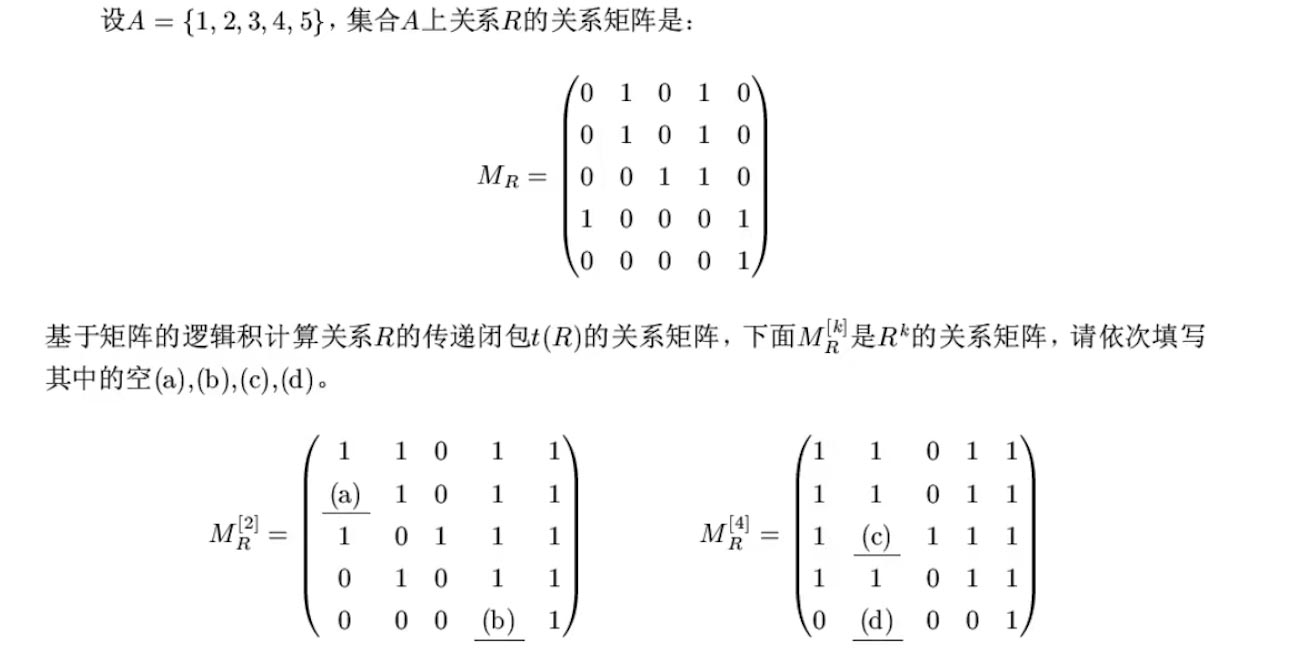
\includegraphics[width=1\textwidth]{6.66.jpg} % 插入图片
    \caption{测验题6.66用图}
\end{figure}

\textcolor{red}{答案:(a)1 (b)0 (c) 1 (d) 0}

\subsubsection{测验题6.67}
\begin{figure}[htbp]
    \centering
    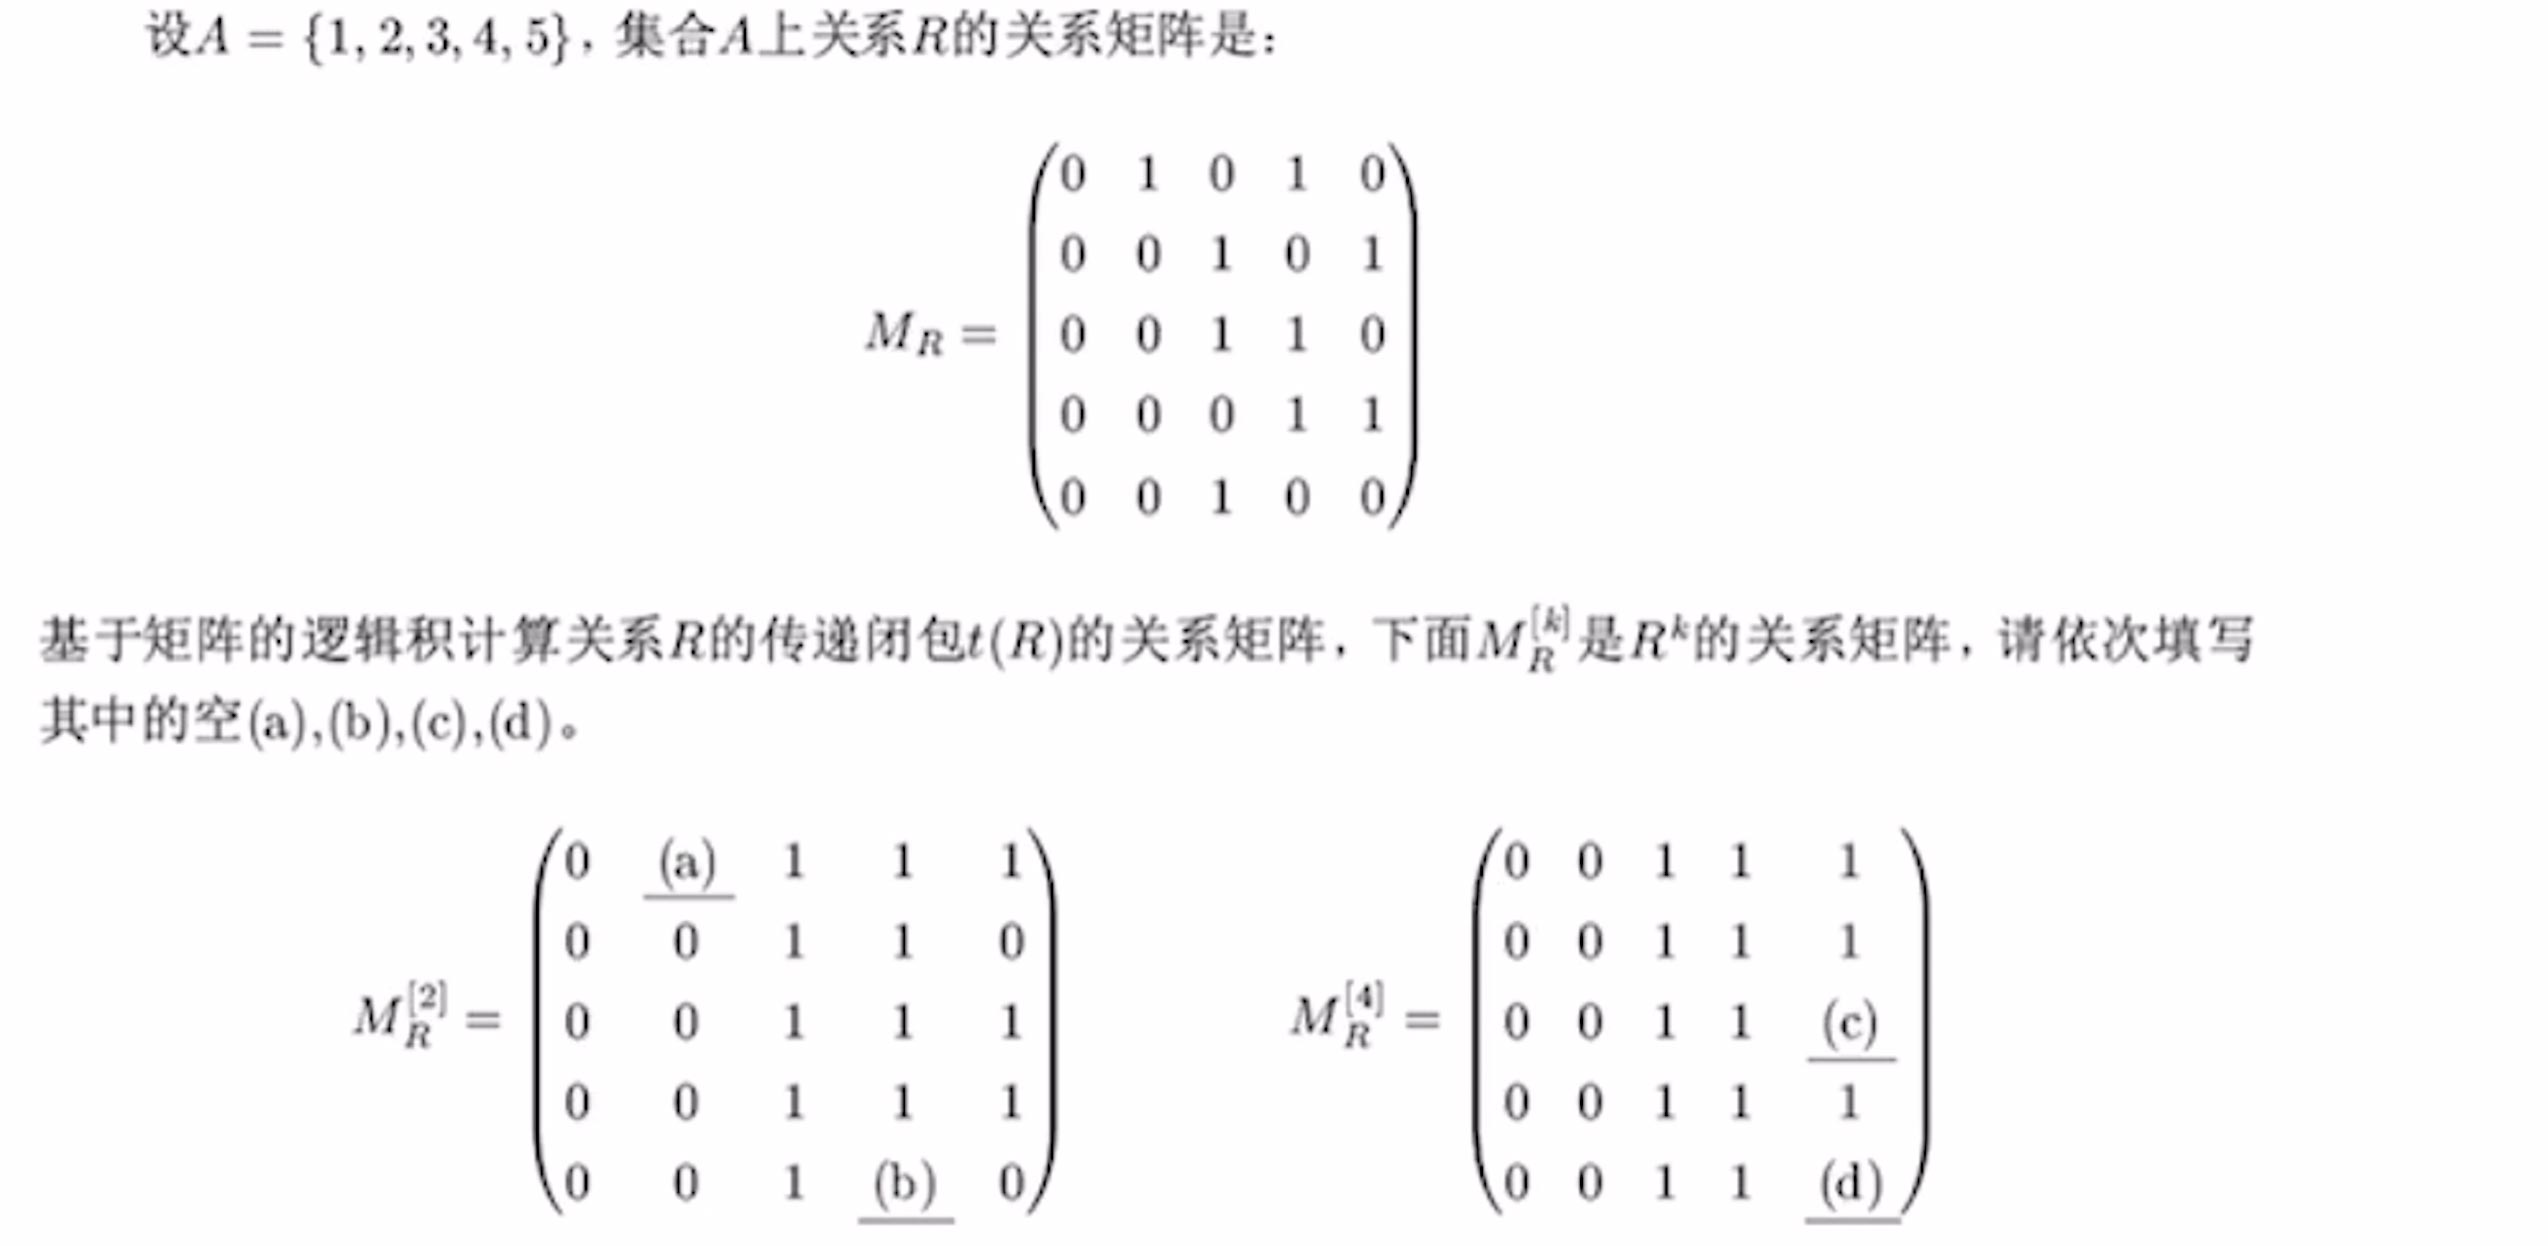
\includegraphics[width=1\textwidth]{6.67.jpg} % 插入图片
    \caption{测验题6.67用图}
\end{figure}

\textcolor{red}{答案:(a)0 (b)1 (c) 1 (d) 1}

\subsubsection{测验题6.69}

\begin{figure}[htbp]
  \centering
  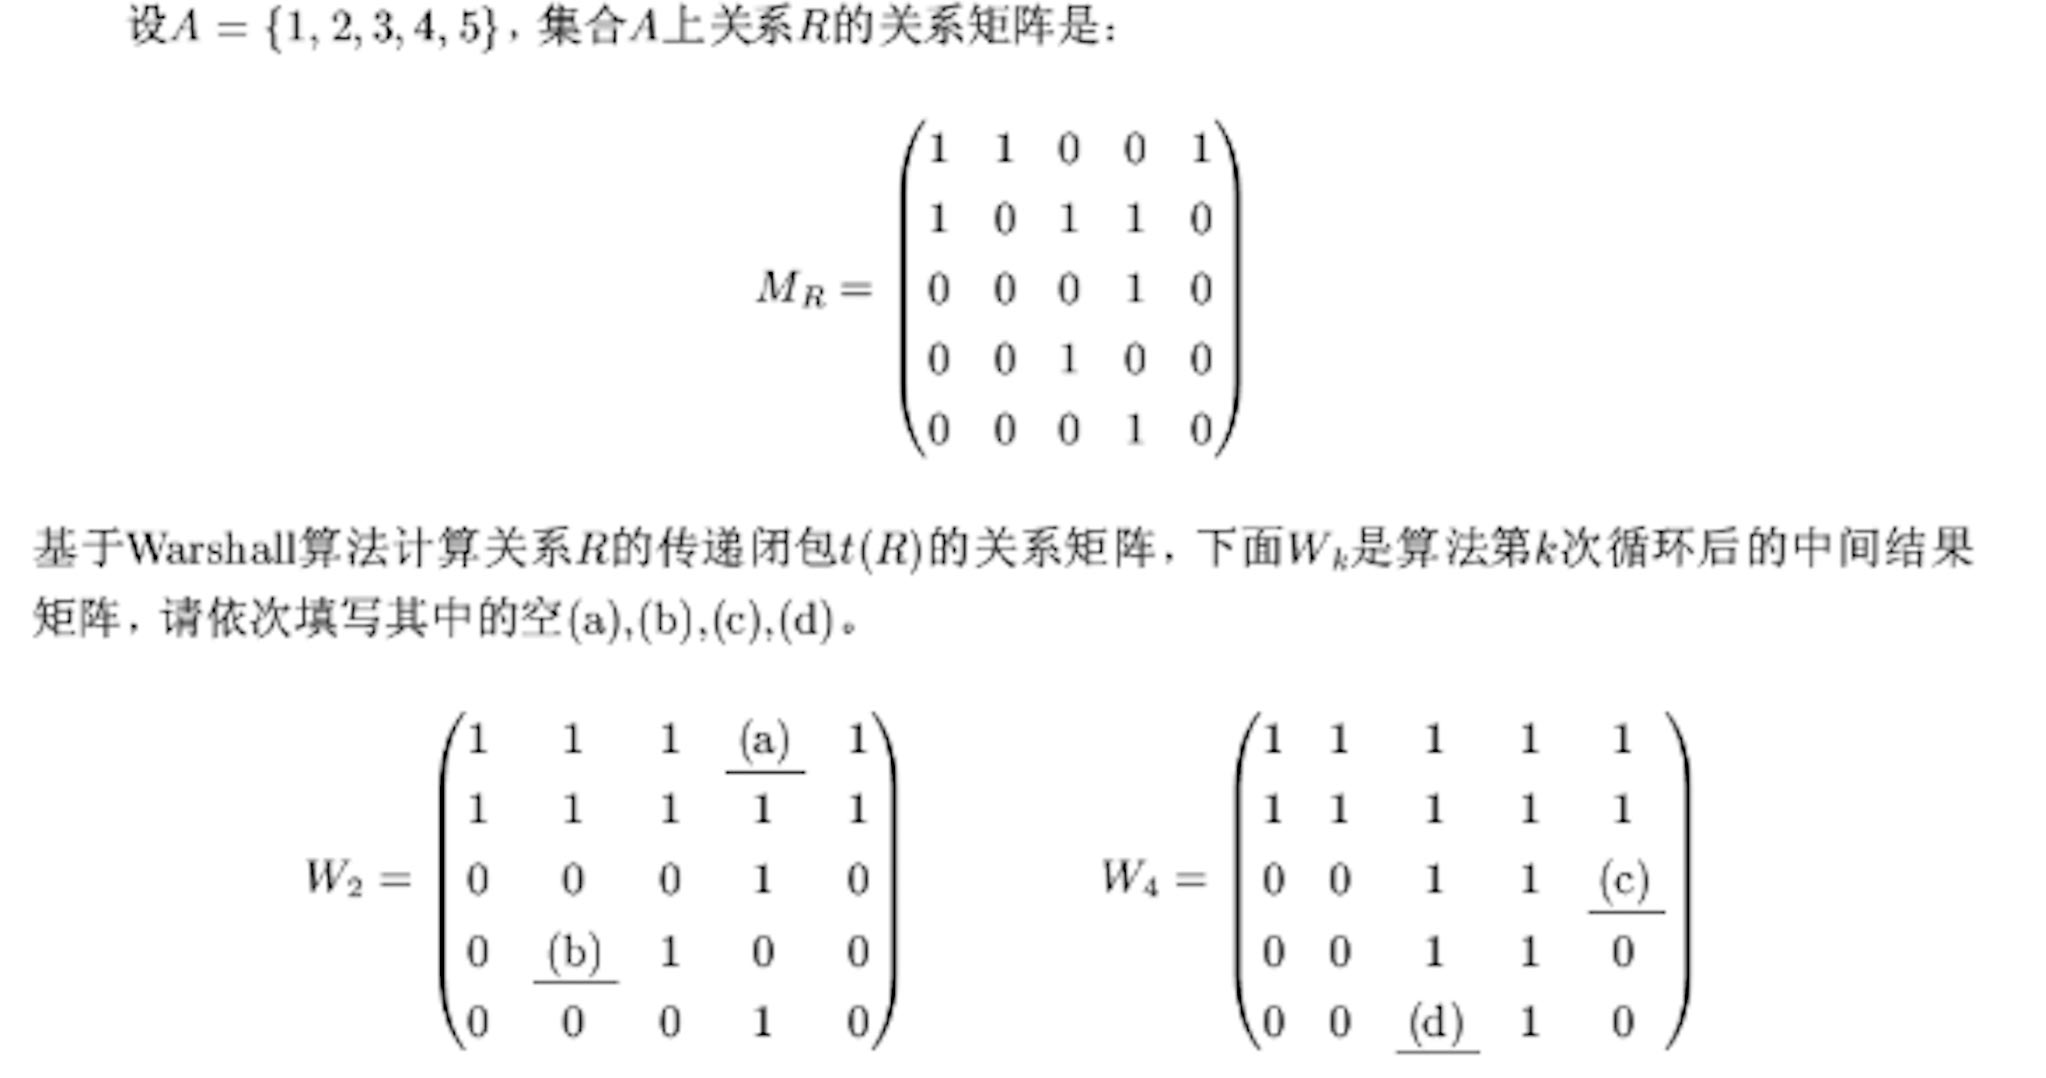
\includegraphics[width=1\textwidth]{6.69.jpg} % 插入图片
  \caption{测验题6.69用图}
\end{figure}

\textcolor{red}{答案:(a)1 (b)0 (c)0 (d) 1}



\subsubsection{测验题6.70}
\begin{figure}[htbp]
    \centering
    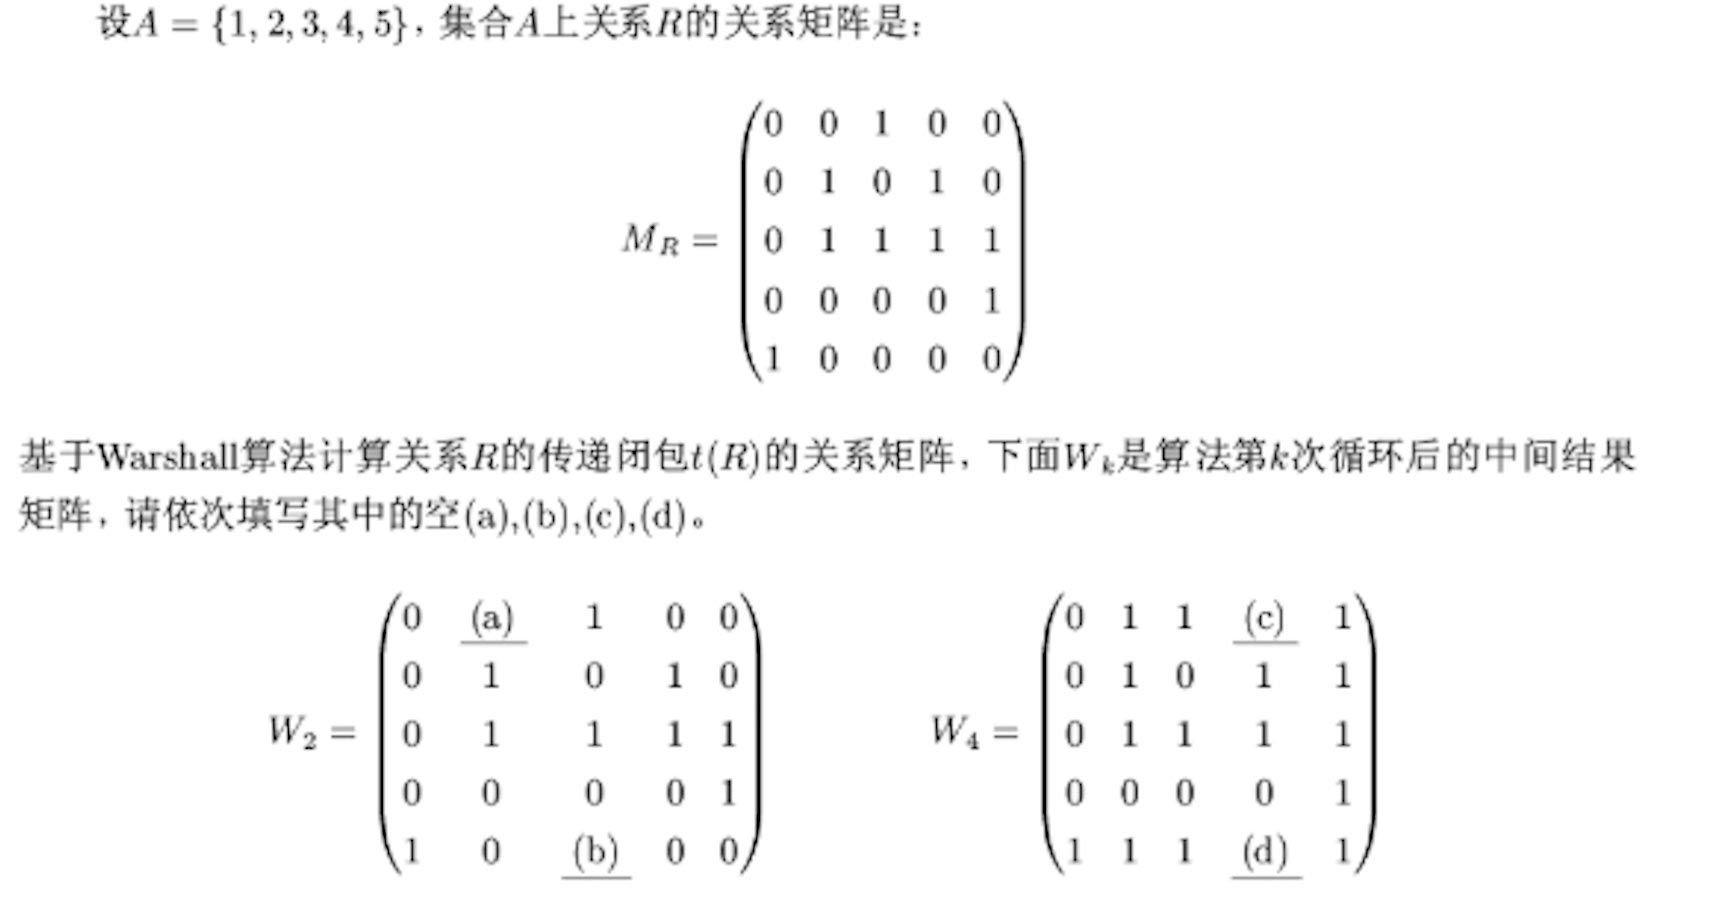
\includegraphics[width=1\textwidth]{6.70.jpg} % 插入图片
    \caption{测验题6.70用图}
\end{figure}

\textcolor{red}{答案:(a)0 (b)1 (c) 1 (d) 1}

\subsubsection{测验题6.72}

设 $R$ 和 $S$ 都是非空集合 $A$ 上的等价关系,下面哪些关系也是等价关系?

A. $R \cup S$

B. $R \cap S$

C. $r(R-S)$

D. $R \circ S$

\textcolor{red}{答案:B}

\textcolor{red}{解析:取$R$为模2同余的关系,$S$为模3同余的关系,则 $\langle 1,3\rangle \in R \cup S$ 且 $\langle 3,6\rangle \in R \cup S$,但是 $\langle 1,6\rangle \notin R \cup S$,所以$R \cup S$不是等价关系,A选项错误;
同理,$\langle 2,4 \rangle \in r(R-S)$且$\langle 4,14 \rangle \in r(R-S)$,但是$\langle 2,14 \rangle \notin r(R-S)$,所以C选项错误。}

\subsubsection{测验题6.73}

设 $A={1,2,3,4}$, 下面哪些关系是集合 $A$ 上的等价关系?

A. $R_1=\{\langle 1,1\rangle,\langle 2,2\rangle,\langle 3,3\rangle,\langle 4,4\rangle\}$

B. $R_2=\Delta_A \cup\{\langle 1,2\rangle,\langle 2,1\rangle\}$

C. 
$R_3=\Delta_A \cup\{\langle 1,2\rangle,\langle 3,4\rangle\}$

D. $R_4=A \times A$

\textcolor{red}{答案:ABD}



\subsubsection{测验题6.74}

设A是中山大学计算机学院所有学生构成的集合,下面哪些关系是集合A上的等价关系?

A. $R_1=\{\langle a, b\rangle \mid a$ 和 $b$ 在相同专业学习 $\}$ (注意每位学生只在学院的一个专业学习)

B. $R_2=\{\langle a, b\rangle \mid a$ 和 $b$ 会用相同编程语言编程 $\}$ (注意一位学生可能会用多门语言编程)

C. $R_3=\{\langle a, b\rangle \mid a$ 和 $b$ 在相同班级学习 $\}$ (注意每位学生只在学院的一个班级学习)

D. $R_4=\{\langle a, b\rangle \mid a$ 和 $b$ 选修了相同课程 $\}$ (注意一位学生可能会选修多门课程)

\textcolor{red}{答案:AC}

\subsubsection{测验题6.75}

下面关于等价类或商集的哪些说法是正确的?

A. 设集合 $A=\{a, b, c\}$ ,则 $A / \Delta_A=\{a, b, c\}$

B. 设集合 $A=\{a, b, c\}$ ,则 $A / A \times A=\{a, b, c\}$

C. 对于集合 $B=\{1,2,3,4\}$ 上的等价关系 $R=\Delta_B \cup\{\langle 2,3\rangle,\langle 3,2\rangle\},[3]_R=\{2,3\}$

D. 对于集合 $B=\{1,2,3,4\}$ 上的关系 $T=\{\langle 1,2\rangle\}$ ,设 $S$ 是包含 $T$ 的最小等价关系,则 $[3]_S=\{3,4\}$

\textcolor{red}{答案:C}


\subsubsection{测验题6.76}

对集合 $A=\{0,1,2,3,4,5\}$ 上的关系 $R=\{(1,2),(4,5)\}$, 设 $T$ 是包含 $R$ 的最小等价关系. 下面关于 $T$ 的等价类的计算哪些是正确的?

A. $[0]_T=\{0,3\}$

B. $[1]_T=\{1,2\}$

C. $[2]_T=\{1,2,4,5\}$

D. $[3]_T=\{3\}$

\textcolor{red}{答案:BD}

\subsubsection{测验题6.80}

在正整数对集 $\mathbb{Z}^{+} \times \mathbb{Z}^{+}$上定义关系 $R=\{\langle\langle a, b\rangle,\langle c, d\rangle\rangle \mid a d=b c\}$ ,可证明 $R$ 是等价关系,下面关于 $R$ 的等价类的说法哪些是正确的?

A. $[1]_R=\mathbb{Z}^{+}$

B. $[\langle 1,1\rangle]_R=\left\{\langle a, a\rangle \mid a \in \mathbb{Z}^{+}\right\}$

C. $\langle 2,1\rangle \in[\langle 1,2\rangle]_R$

D. $\langle 3,9\rangle \in[\langle 1,3\rangle]_R$

\textcolor{red}{答案:BD}

\subsubsection{测验题6.82}

设集合A是所有长度为8的所有三进制串构成的集合,下面哪些集合族是A的划分?

A. $\mathcal{F}_1=\{$ 所有以 0 开头的串构成的集合,所有以 1 开头的串构成的集合,所有以 20 开头的串构成的集合, 所有以 21 开头的串构成的集合, 所有以 22 开头的串构成的集合 $\}$

B. $\mathcal{F}_2=\{$ 所有包含饸好一个 0 的串构成的集合,所有包含恰好一个 1 的串构成的集合,所有包含恰好一个 2 的串构成的集合 $\}$

C. $\mathcal{F}_3=\{$ 所有以 00 结尾的串构成的集合, 所有以 01 结尾的串构成的集合, 所有以 02 结尾的串构成的集合,所有以 1 结尾的串构成的集合,所有以 2 结尾的串构成的集合 $\}$

D. $\mathcal{F}_4=\{$ 所有恰好含有偶数个 0 的串构成的集合,所有恰好含有偶数个 1 的串构成的集合, 所有恰好含有偶数个 2 的串构成的集合 $\}$

\textcolor{red}{答案:A}

\subsubsection{测验题6.83}
设集合 $A={0,1,2,3,4,5}$, 下面哪些集合族是 $A$ 的划分?

A. $\mathcal{F}_1=\{0,1,2,3,4,5\}$

B. $\mathcal{F}_2=\{\{0,1\},\{4,5\}\}$

C. $\mathcal{F}_3=\{\{0,1,2\},\{3,4,5\}\}$

D. $\mathcal{F}_4=\{\{0\},\{1\},\{2\},\{3\}\}$

\textcolor{red}{答案:C}

\subsubsection{测验题6.86}

设 $R$ 和 $S$ 都是非空集合 $A$ 上的偏序关系,下面哪些关系也是A上的偏序关系?

A. $R \cap S$

B. $R \cup S$

C. $r(R-S)$

D. $R \circ S$

\textcolor{red}{答案:A}


\subsubsection{测验题6.87}

设 $A=\{1,2,3,4\}$ ,下面哪些关系是集合 $A$ 上的偏序关系?


A. $
R_1=\{\langle 1,1\rangle,\langle 2,2\rangle,\langle 3,3\rangle,\langle 4,4\rangle\}
$

B. $R_2=\Delta_A \cup\{\langle 1,2\rangle,\langle 2,1\rangle\}$

C. $R_3=\Delta_A \cup\{\langle 1,2\rangle,\langle 3,4\rangle\}$

D. $R_4=A \times A$

\textcolor{red}{答案:AC}

\subsubsection{测验题6.90}

设A是偏序集,下面哪些说法是正确的?

A. 偏序集A的极大元存在的话一定也是它的最大元

B. 偏序集A的最小元存在的话一定也是它的极小元

C. 偏序集A至多存在一个最小元

D. 偏序集A可能同时存在无穷多个极大元和极小元

\textcolor{red}{答案:BCD}

\subsubsection{测验题6.91}

设A是偏序集,S是A的子集,下面哪些说法是正确的?

A. 子集S如果存在最大元,则S必存在上确界

B. 子集S如果存在一个属于S的下界,则S必存在下确界

C. 子集 $S$ 的所有上界都必然属于 $S$

D. 如果A存在最小元,则S一定有下确界

\textcolor{red}{答案:AB}

\subsubsection{测验题6.93}

设集合 $A=\{n \in N \mid n$ 是 60 的正因子 $\}$ 以整除关系为偏序构成偏序集,下面㗖些说法是正确的?

A. 偏序集A的最小元是1

B. 偏序集A的最大元是 60

C.  $60,30,20,10$ 都是偏序集A的极大元

D. $1,2,3,4,5$ 都是偏序集 $A$ 的极小元

\textcolor{red}{答案:AB}




\clearpage

\section{函数}


\subsubsection{测验题7.6}

下面定义的集合 $A$ 到 $B$ 的函数哪些是单函数?

A. 集合 $A=\{1,2,3,4,5\}, B=\{a, b, c, d\}$ ,函数 $f_1=\{\langle 1, b\rangle,\langle 2, c\rangle,\langle 3, a\rangle,\langle 4, c\rangle,\langle 5, c\rangle\}$

B. 集合 $A=\{1,2,3,4,5\}, B=\{a, b, c, d\}$ ,函数 $f_2=\{\langle 1, d\rangle,\langle 2, b\rangle,\langle 3, b\rangle,\langle 4, c\rangle,\langle 5, a\rangle\}$

C. 集合 $A=\{1,2,3,4\}, B=\{a, b, c, d\}$ ,函数 $f_3=\{\langle 1, a\rangle,\langle 2, d\rangle,\langle 3, c\rangle,\langle 4, b\rangle\}$

D. 集合 $A=\{1,2,3\}, B=\{a, b, c, d, e\}$ ,函数 $f_4=\{\langle 1, e\rangle,\langle 2, d\rangle,\langle 3, b\rangle\}$

\textcolor{red}{答案:CD}

\subsubsection{测验题7.11}

下面定义从自然数集$\mathbb{N}$到整数集$\mathbb{Z}$的函数哪些是双函数?

A. 函数 $f_1(n)=2 n+1$

B. 函数 $f_2(n)=\lfloor(n+1) / 2\rfloor$

C. 函数 $f_3(n)=\lceil(2 n+1) / 2\rceil$

D. 函数 $f_4(n)= \begin{cases}-k & \text { 若 } n=2 k-1, k \geq 1 \\ k & \text { 若 } n=2 k\end{cases}$

\textcolor{red}{答案:D}

\subsubsection{测验题7.12}

下面函数都是实数集$\mathbb{R}$上的函数,下面哪些对函数性质的判断是正确的?

A. 函数 $f_1(x)=x^2$ 是单函数

B. 函数 $f_2(x)=x^3$ 是单函数

C. 函数 $f_3(x)=\lfloor x\rfloor$ 是满函数

D. 函数 $f_4(x)=2 x+1$ 是满函数

\textcolor{red}{答案:BD}

\subsubsection{测验题7.13}

下面函数都是从自然数对集 $\mathbb{N} \times \mathbb{N}$ 到自然数集 $\mathbb{N}$ 的函数,下面哪些对函数性质的判断是正确的?

A. 函数 $f_1(m, n)=m^2+n^2$ 是单函数

B. 函数 $f_2(m, n)=|m-n|$ 是单函数

C. 函数 $f_3(m, n)=\lfloor(m+n) / 2\rfloor$ 是满函数

D. 函数 $f_4(m, n)=m$ 是满函数

\textcolor{red}{答案:CD}

\subsubsection{测验题7.15}

设下面对函数$f$和$g$所做的函数复合都是可行的,下面哪些说法是正确的?

A. 函数 $g \circ f$ 是单函数,则函数 $f$ 和 $g$ 也都是单函数

B. 函数 $f$ 和 $g$ 都是满函数,则函数 $g \circ f$ 也是满函数

C. 函数 $g \circ f$ 是双函数,则函数 $f$ 是双函数

D. 函数 $g \circ f$ 是满函数,则函数 $g$ 也是满函数

\textcolor{red}{答案:BD}

\subsubsection{测验题7.22*}

下面哪些说法是正确的?

A. 所有偶自然数构成的集合是自然数集的子集,因此它不与自然数集等势

B. 实数集的开区间 $(0,1)$ 是开区间 $(-1,1)$ 的子区间,因此这两个区间不等劸

C. 所有偶自然数构成的集合与所有 3 的倍数的自然数构成的集合等势

D. 然数集与正整数集等势

\textcolor{red}{答案:CD}

\subsubsection{测验题7.24*}

下面关于有穷集的哪些说法是正确的?

A. 有穷集与某个自然数等势

B. 如果一个集合的任意真子集都是有穷集,则这个集合也是有穷集

C. 如果一个集合的某个真子集是有穷集,则这个集合就是有穷集

D. 有穷集不与它的任何真子集等势

\textcolor{red}{答案:ABD}


\subsubsection{测验题7.26*}

下面关于可数集和不可数集的哪些说法是正确的?

A. 可数集一定是有穷集

B. 不可数集一定是无穷集

C. 有穷集一定是可数集

D. 无穷集一定是不可数集

\textcolor{red}{答案:BC}

\subsubsection{测验题7.28*}

下面哪些集合是可数集?

A. 空集 $\varnothing$

B. 自然数 $n$

C. 自然数集 $\mathbb{N}$

D. 自然数集的幂集 $\wp(\mathbb{N})$

\textcolor{red}{答案:ABC}

\subsubsection{测验题7.29*}

下面哪些集合不是可数集?

A. 自然数对集 $\mathbb{N} \times \mathbb{N}$

B. 有理数对集 $\mathbb{Q} \times \mathbb{Q}$

C. 实数对集 $\mathbb{R} \times \mathbb{R}$

D. 正整数集上的所有函数构成的集合 $\mathbb{Z}^Z$

\textcolor{red}{答案:CD}

\subsubsection{测验题7.34}

假设下面函数都是数集上的函数,哪些函数是 $O(x)$ ?

A. $f_1(x)=100$

B. $f_2(x)=100 x+123$

C. $f_3(x)=x^2+2 x+1$

D. $f_4(x)=2 \log x+1$

\textcolor{red}{答案:ABD}

\subsubsection{测验题7.38}

下面哪些说法是正确的?

A. $ n \log n \in O\left(n^3\right)$

B. $2^n \in O(n!)$

C. $n^2 \in O\left(n^4\right)$

D. $ n \in O\left(\log n^2\right)$

\textcolor{red}{答案:ABC}

\subsubsection{测验题7.40}

对于函数 $f(n)=\left(n^4+n^2 \log n\right) /\left(n^2+(\log n)^2\right)$ ,下面哪些说法是正确的?

A. $ f \in O\left(n^4\right)$

B. $ f \in O\left(n^2\right)$

C. $ f \in O(n \log n)$

D. $f \in O(n)$

\textcolor{red}{答案:AB}


\subsubsection{测验题7.41}

对于函数 $f(x)=\left(x \log x+x^2\right)(x+2)$ ,下面吸些说法是正确的?

A. $ f \in O(x \log x)$

B. $f \in O\left(x^2 \log x\right)$

C. $f \in O\left(x^3 \log x\right)$

D. $ f \in O\left(x^3\right)$

\textcolor{red}{答案:CD}

\subsubsection{测验题7.44}

对于函数 $f(x)=\left(2 x^4+4 x^2+2 x\right) /\left(x^3+3 x^2+1\right)$ ,下面哪些说法是正确的?

A. $f \in O(x)$ 且 $f \notin O(1)$

B. $f \in O\left(x^2\right)$ 且 $f \notin O(x)$

C. $f \in O\left(x^3\right)$ 且 $f \notin O\left(x^2\right)$

D. $\quad f \in O\left(x^4\right)$ 且 $f \notin O\left(x^3\right)$

\textcolor{red}{答案:A}




\clearpage
\section{计数与组合}

\subsubsection{测验题8.1}

设全集U是四位数(这一题所说的数都是指自然数)构成的集合,A是四位数奇数构成的集合,B是四位数偶数构成的集合,
C是含有奇数数字的四位数构成的集合,D是含有偶数数字的四位数构成的集合,E是只含有奇数数字的四位数构成的集合,F是只含有偶数数字的四位数构成的集合。下面哪些说法是正确的?

A. 根据加法原理, $|U|=|A|+|B|$

B. 根据加法原理, $|U|=|C|+|D|$

C. 根据加法原理, $|U|=|E|+|F|$

D. 根据加法原理, $|U|=|C|+|F|$

\textcolor{red}{答案:AD}

\subsubsection{测验题8.2}

设全集U是长度为8的小写英文字母串构成的集合,A是U中含有元音字母的串构成的集合,B是U中含有辅音字母的串构成的集合,C是U中以元音字母开头的串构成的集合,D是U中以辅音字母开头的串构成的集合,E是U中只含有元音字母的串构成的集合,F是U中只含有辅音字母的串构成的集合。下面哪些说法是正确的?

A. 根据加法原理, $|U|=|A|+|B|$

B. 根据加法原理, $|U|=|C|+|D|$

C. 根据加法原理, $|U|=|E|+|F|$

D. 根据加法原理, $|U|=|A|+|F|$

\textcolor{red}{答案:BD}

\subsubsection{测验题8.3}

设计算机学院有计算机系统、计算机软件和计算机应用三个专业。令全集U是从计算机学院这三个专业学生中推选10位学生干部的所有不同方案构成的集合,A是U中含有计算机系统专业学生的方案构成的集合,B是U中含有计算机软件专业学生的方案构成的集合,C是U中含有计算机应用专业学生的方案构成的集合,D是U中只含有计算机系统专业学生的方案构成的集合,E是U中只含有计算机软件专业学生的方案构成的集合,F是U中只含有计算机应用专业学生的方案构成的集合,G是U中恰好含有一个专业学生的方案构成的集合,H是U中恰好含有两个专业学生的方案构成的集合,I是U中恰好含有三个专业学生的方案构成的集合。下面哪些说法是正确的?

A. 根据加法原理, $|U|=|A|+|B|+|C|$

B. 根据加法原理, $|U|=|D|+|E|+|F|$

C. 根据加法原理, $|U|=|G|+|H|+|I|$

D. 根据加法原理, $|G|=|D|+|E|+|F|$

\textcolor{red}{答案:CD}
\subsubsection{测验题8.4}
计算只含奇数数字的四位数个数,将确定四位数的个位、十位、百位和千位看做子任务,下面哪些说法是正确的?

A. 按照确定个位、十位、百位、千位的顺序考虑,这些子任务之间具有相关性。

B. 按照确定千位、百位、十位、个位的顺序考虑,这些子任务之间具有相关性。

C. 按照确定个位、十位、百位、千位的顺序考虑,这些子任务之间具有独立性。

D. 按照确定千位、百位、十位、个位的顺序考虑,这些子任务之间具有独立性。

\textcolor{red}{答案:CD}

\subsubsection{测验题8.5}

计算只含偶数数字的四位数个数,将确定四位数的个位、十位、百位和千位看做子任务,下面哪些说法是正确的?

A. 按照确定个位、十位、百位、千位的顺序考虑,这些子任务之间具有相关性。

B. 按照确定千位、百位、十位、个位的顺序考虑,这些子任务之间具有相关性。

C. 按照确定个位、十位、百位、千位的顺序考虑,这些子任务之间具有独立性。

D. 按照确定千位、百位、十位、个位的顺序考虑,这些子任务之间具有独立性。

\textcolor{red}{答案:CD}

\subsubsection{测验题8.6}

计算只含奇数数字且数字不同的四位数个数,将确定四位数的个位、十位、百位和千位看做子任务,下面哪些说法是正确的?

A. 按照确定个位、十位、百位、千位的顺序考虑,这些子任务之间具有相关性。

B. 按照确定千位、百位、十位、个位的顺序考虑,这些子任务之间具有相关性。

C. 按照确定个位、十位、百位、千位的顺序考虑,这些子任务之间具有独立性。

D. 按照确定千位、百位、十位、个位的順序考虑,这些子任务之间具有独立性。

\textcolor{red}{答案:ABCD}

\subsubsection{测验题8.7}
计算只含偶数数字且数字不同的四位数个数,将确定四位数的个位、十位、百位和千位看做子任务,下面哪些说法是正确的?

A. 按照确定个位、十位、百位、千位的顺序考虑,这些子任务之间具有相关性。

B. 按照确定千位、百位、十位、个位的顺序考虑,这些子任务之间具有相关性。

C. 按照确定个位、十位、百位、千位的顺序考虑,这些子任务之间具有独立性。

D. 按照确定千位、百位、十位、个位的顺序考虑,这些子任务之间具有独立性。

\textcolor{red}{答案:ABD}

\subsubsection{测验题8.8}
计算数字不同的四位数, 下面哪些说法是正确的?

A. 可以按确定个位、十位、百位、千位的顺序考虑, 分别有 $10,9,8,7$ 个可选数字, 因此共有 $10^* 9 ^* 8^* 7$ 个。

B. 可以按确定千位、百位、十位、个位的顺序考虑, 分别有 $9,9,8,7$ 个可选数字,因此共有 $9^* 9^* 8^* 7$ 个。

C. 可以按确定个位、千位、百位、十位的顺序考虑, 分别有 $10,8,8,7$ 个可选数字, 因此共有 $10^* 8^* 8^* 7$ 个。

D. 可以按确定千位、个位、百位、十位的顺序考虑,分别有 $9,9,8,7$ 个可选数字,因此共有 $9^* 9^* 8^* 7$ 个。

\textcolor{red}{答案:BD}

\subsubsection{测验题8.9}

计算数字不同的四位数奇数,下面哪些说法是正确的?

A. 可以按确定个位、十位、百位、千位的顺序考虑,分别有 $5,9,8,6$ 个可选数字,因此共有 $5^* 9^* 8^* 6$ 个。

B. 可以按确定千位、百位、十位、个位的顺序考虑, 分别有 $9,9,8,5$ 个可选数字, 因此共有 $9 ^* 9 ^* 8 ^* 5$ 个。

C. 可以按确定个位、千位、百位、十位的顺序考虑,分别有 $5,8,8,7$ 个可选数字,因此共有 $5 ^* 9 ^* 8 ^* 7$ 个。

D. 可以按确定千位、个位、百位、十位的顺序考虑, 分别有 $9,5,8,7$ 个可选数字, 因此共有 $9 ^* 5^* 8^* 7$ 个。

\textcolor{red}{答案:C}

\textcolor{red}{解析:C选项的结果应为$5^* 8 ^* 8 ^* 7$}

\subsubsection{测验题8.10}

计算数字不同的四位数偶数,下面哪些说法是正确的?

A. 可以按确定个位、十位、百位、千位的顺序考虑, 分别有 $5,9,8,6$ 个可选数字, 因此共有 $5^* 9^* 8^* 6$ 个。

B. 可以按确定千位、百位、十位、个位的顺序考虑,分别有 $9,9,8,5$ 个可选数字,因此共有 $9^* 9^* 8^* 5$ 个。

C. 可以按确定个位、千位、百位、十位的顺序考虑, 个位选 0 , 则千位、百位、十位分别有 $9,8,7$ 个可选数字, 个位不选 0 , 则个位、千位、百位、十位分别有 $4,8,8,7$ 个可选数字, 因此共有 $1 ^* 9^* 8^* 7+4^* 8^* 8^* 7$ 个。

D. 可以按确定千位、个位、百位、十位的顺序考虑,千位选偶数,则千位、个位、百位、十位分别有 $4,4,8,7$ 个可选数字,千位选奇数,则千位、个位、百位、十位分别有 $5,5,8,7$ 个可选数字, 因此共有 $4^* 4^* 8^* 7+5^* 5^* 8^* 7$ 个。

\textcolor{red}{答案:CD}

\subsubsection{测验题8.11}

使用减法原理计算满足条件的四位数个数,下面哪些是正确的?

A. 用数字不同的四位数总数减去数字不同的四位数奇数个数得到数字不同的四位数偶数个数。

B. 用四位数总数减去含有奇数数字的四位数个数得到含有偶数数字的四位数个数。

C. 用四位数总数减去含有数字 0 的四位数个数得到不含数字 0 的四位数个数。

D. 用四位数总数减去含有数字 0 的四位数个数, 再减去含有数字 1 的四位数个数, 得到不含有数字 0 或不含有数字 1 的四位数个数。

\textcolor{red}{答案:AC}

\subsubsection{测验题8.12}

计算机学院有计算机系统、计算机软件和计算机应用三个专业的学生,要推选10位学生担任学生干部。使用减法原理计算推选方案数,下面哪些是正确的?

A. 总的推选方案数减去含有计算机系统专业学生的推选方案数得到只含有计算机软件或计算机应用专业学生的推选方案数。

B. 总的推选方案数减去含有男生的推选方案数得到只含有女生的推选方案数。

C. 总的推选方案数减去含有计算机系统专业学生的推选方案数, 再减去含有计算机软件专业学生的推选方案数, 得到只含有计算机应用专业学生的推选方案数。

D. 总的推选方案数减去含有计算机系统专业男生的推选方案数得到含有计算机系统专业女生的推选方案数。

\textcolor{red}{答案:AB}

\textcolor{red}{解析:C选项同时选中计算机系统与计算机软件专业的情况被重复减去。}

\subsubsection{测验题8.13}

自然数的三位数中只含奇数数字的有(1)个,只含偶数数字的有(2)个,只含奇数数字且数字不同的有(3)个,只含偶数数字且数字不同的有(4)个(直接填写结果)。

\textcolor{red}{答案:(1) 125 (2) 100 (3) 60 (4) 48}


\subsubsection{测验题8.14}
自然数的三位数中含有奇数数字的有(1)个,含有偶数数字的有(2)个,含有数字0的有(3)个,含有数字1的有(4)个(直接填写结果)。

\textcolor{red}{答案:(1) 800 (2) 775 (3) 171 (4) 252}

\subsubsection{测验题8.15}

自然数中数字不同的三位数有(1)个,数字不同的三位数奇数有(2)个,数字不同的三位数偶数有(3)个(直接填写结果)。

\textcolor{red}{答案:(1) 648 (2) 320 (3) 328}

\subsubsection{测验题8.16}

由0,1,2,3,4这五个数字能组成的三位数有(1)个,其中数字不同的有(2)个。由0,1,2,3,4这五个数字能组成的大于210的三位数有(3)个,其中数字不同的又有(4)个(直接填写结果)。

\textcolor{red}{答案:(1) 100 (2) 48 (3) 69 (4) 32}

\subsubsection{测验题8.17}

计算机学院有计算机软件专业40名学生,其中男女学生各20名,计算机应用专业20名学生,其中男女学生各10名。现在要推选一位学生任学生会主席,则有(1)种推选方法。如果要推选一位学生任主席,
另一位任副主席则有(2)种推选方法,
其中主席和副主席来自不同专业的推选方法有(3)种,而主席和副主席来
自不同专业且性别也不同的推选方法有(4)种(直接填写结果)。

\textcolor{red}{答案:(1) 60 (2) 3540 (3) 1600 (4) 800}

\subsubsection{测验题8.18}

整数 $3^4 \times 5^2 \times 7^6 \times 11$ 有(1)个正因子, 整数 620有 (2)个正因子,
而整数 $10^{10}$ 有(3)个正因子。

\textcolor{red}{答案:(1) 210 (2) 12 (3) 121}

\textcolor{red}{解析:\newline(1)结论:指数加一再连乘。 例如对于$3^4 \times 5^2 \times 7^6 \times 11$,
共有$(4+1) \times (2+1) \times (6+1) \times (1+1)=210$个正因子。
结论的理解也比较直观,对于$3^4$这一项,它能分解出的因子有$3^0,3^1,3^2,3^3,3^4$共5个,对于$5^2$这一项,它能分解出的因子有$5^0,5^1,5^2$共3个,以此类推。
从每一项中选出一种因子分解再乘起来即为答案。\newline (2)$620=2^2 \times 5 \times 31$,共有$(2+1) \times (1+1) \times (1+1)=12$}


\subsubsection{测验题8.19}

假定全集是U,A, B, C都是U的任意子集,下面关于集合元素个数的等式哪些是正确的?

A. $|A \cap \bar{B}|=|A|-|B|$

B. $|\bar{A} \cap \bar{B}|=|U|-|A|-|B|+|A \cap B|$

C. $|A \cap B \cap \bar{C}|=|A \cap B|-|A \cap B \cap C|$

D. $|A \cap \bar{B} \cap \bar{C}|=|A|-|B|-|C|+|B \cap C|$

\textcolor{red}{答案:BC}

\subsubsection{测验题8.20}

假定全集是U,A, B, C都是U的任意子集,下面关于集合元素个数的等式哪些是正确的

A. $|A \cup \bar{B}|=|U|-|B|+|A \cap B|$

B. $|\bar{A} \cup \bar{B}|=|U|-|A \cap B|$

C. $|A \cup B \cup \bar{C}|=|A|+|B|-|C|$

D. $|A \cup \bar{B} \cup \bar{C}|=|A|-|B|-|C|+|B \cap C|$

\textcolor{red}{答案:AB}

\subsubsection{测验题8.21}

假定全集U是正整数集,集合A是能被3整除的正整数集合,集合B是能被5整除的正整数集合,集合C是能被7整除的正整数集合,下面哪些说法是正确的?

A. 能被 3 或 5 整除的正整数集合是 $A \cup B$

B. 能被 $3,5,7$ 之一整除的正整数集合是 $A \cup B \cup C$

C. 不能被 3 或 5 整除的正整数集合是 $\bar{A} \cup \bar{B}$

D. 不能被 3,5 或 7 之一整除的正整数集合是 $\bar{A} \cup \bar{B} \cup \bar{C}$

\textcolor{red}{答案:AB}

\subsubsection{测验题8.22}

假定全集U是正整数集,集合A是能被3整除的正整数集合,集合B是能被5整除的正整数集合,集合C是能被7整除的正整数集合,下面哪些说法是正确的?

A. 能同时被 3 和 5 整除的正整数集合是 $A \cap B$

B. 能被 3 整除, 但不能被 5 整除的正整数集合是 $A \cup \bar{B}$

C. 或者被 3 整除, 或者被 5 整除, 或者不被 7 整除的正整数集合是 $A \cup B \cup \bar{C}$

D. 能同时被 3 和 5 整除, 但不能被 7 整除的正整数集合是 $A \cap B \cup \bar{C}$

\textcolor{red}{答案:AC}
\subsubsection{测验题8.23}

假定全集U是计算机学院所有学生,集合A是选修了数理逻辑课程的学生,集合B是选修了数论课程的学生,集合C是选修了抽象代数课程的学生,下面哪些说法是正确的?

A. 选修了数理逻辑、数论或抽象代数课程的学生集合是 $A \cup B \cup C$

B. 只选修了数理逻辑而没有选修其他两门课程的学生集合是 $A \cap \overline{B \cap C}$

C. 选修了数理逻辑或者没有选修抽象代数课程的学生集合是 $A \cap \bar{C}$

D. 选修了数理逻辑或数论, 但没有选修抽象代数课程的集合是 $(A \cup B) \cap \bar{C}$

\textcolor{red}{答案:AD}

\subsubsection{测验题8.24}
假定全集U是所有三位正整数构成的集合,集合A是能被3整除的正整数集合,集合B是能被5整除的正整数集合,集合C是能被7整除的正整数集合,下面哪些计算是正确的?

A. $|A|=\lfloor(999-100) / 3\rfloor=300$

B. $|B|=\lfloor 999 / 5\rfloor-\lfloor 99 / 5\rfloor=180$

C. $|A \cap \bar{B}|=\lfloor 999 / 3\rfloor-\lfloor 99 / 3\rfloor-\lfloor 999 / 15\rfloor+\lfloor 99 / 15\rfloor=240$

D. $|A \cap \bar{B} \cap \bar{C}|=\lfloor 999 / 3\rfloor-\lfloor 99 / 3\rfloor-\lfloor 999 / 15\rfloor+\lfloor 99 / 15\rfloor-\lfloor 999 / 21\rfloor+\lfloor 99 / 21\rfloor=197$

\textcolor{red}{答案:BC}

\subsubsection{测验题8.25}

假定全集U是所有三位正整数构成的集合,集合A是能被2整除的正整数集合,集合B是能被4整除的正整数集合,集合C是能被6整除的正整数集合,下面哪些计算是正确的?

A. $|A|=\lfloor(999-100) / 2\rfloor=450$

B. $|A \cap B|=\lfloor 999 / 8\rfloor-\lfloor 99 / 8\rfloor=112$

C. $|B \cap C|=\lfloor 999 / 12\rfloor-\lfloor 99 / 12\rfloor=75$

D. $|A \cap B \cap C|=\lfloor 999 / 48\rfloor-\lfloor 99 / 48\rfloor=18$

\textcolor{red}{答案:C}

\textcolor{red}{解析:A选项结果计算正确但是计算过程有误,应该是$|A|=\lfloor 999 / 2\rfloor - \lfloor 99 / 2\rfloor=450$}

\subsubsection{测验题8.26}


能被2或3整除的三位正整数有(1)个,能被5但不能被7整除的三位正整数有(2)个,不能被3或5整除的三位正整数有(3)个(直接填写结果)。

\textcolor{red}{答案:(1) 600 (2) 154 (3) 480}

\subsubsection{测验题8.27}
能被4或6整除的三位正整数有(1)个,能被4但不能被6整除的三位正整数有(2)个
,不能被4整除或者不能被6整除的三位正整数有(3)个(直接填写结果)。

\textcolor{red}{答案:(1) 300 (2) 150 (3) 825}

\subsubsection{测验题8.28}

长度为6的二进制串以1开头的有(1)个,长度为6的二进制串以01结束的有(2)个,长度为6的二进制串以1开头或者以01结束的有(3)个(直接填写结果)。

\textcolor{red}{答案:(1) 32 (2) 16 (3) 40}

\subsubsection{测验题8.29}

长度为5的三进制串以1开头的有(1)个,
长度为5的三进制串以01结束的有(2)个,
长度为5的三进制串以1开头或者以01结束的有(3)个(直接填写结果)。

\textcolor{red}{答案:(1) 81 (2) 27 (3) 99}

\subsubsection{测验题8.30}

计算机学院一个班40名学生中有20人选修数理逻辑课程,15人选取数论课程,
有5人同时选修了这两门课程,则这两门课程都没有选修的学
生有(1)人,只选修数理逻辑而没有选数论课程的学
生有(2)人,只选修了数论而没有选修数理逻辑课程的学生有(3)人。

\textcolor{red}{答案:(1) 10 (2) 15 (3) 10}

\subsubsection{测验题8.31}

假定计算机学院每位学生必须至少选修数理逻辑、
数论和抽象代数三门课程之一。已知选修数理逻辑课程的学生有170人,
选修数论课程的学生有130人,选修抽象代数课程的学生有120人,同时选修
数理逻辑和数论课程的学生有50人,同时选修数理逻辑和抽象代数的学生有20人,同时选
修数论和抽象代数课程的学生有25人,三门课程都选修的学生有5人,则计算机学院总共
有(1)位学生,其中只选修了数理逻辑课程的学生有(2)人,
只选修了数论课程的学生有(3)人,只选修了抽象代数课程的学生有(4)人。

\textcolor{red}{答案:(1) 330 (2) 105 (3) 60 (4) 80}


\subsubsection{测验题8.32}

含有数字0的三位正整数有(1)个,
含有数字1的三位正整数有(2)个,
含有数字0或数字1的三位正整数有(3)个。

\textcolor{red}{答案:(1) 171 (2) 252 (3) 388}

\subsubsection{测验题8.33}

如果一个班级每周班会的时间经常变动,那么需要至少(1)周,才能保证至少有两次班会的时间一周的同一天(例如同是星期一)召开。

\textcolor{red}{答案:(1) 8}


\subsubsection{测验题8.34}

至少需选取(1)个正整数才能保证其中至少有2个正整数的差是10的倍数。

\textcolor{red}{答案:(1) 11}

\subsubsection{测验题8.35}
至少需选取(1)个正整数才能保证其中至少有10个正整数整除7的余数都相同。

\textcolor{red}{答案:(1) 64}

\subsubsection{测验题8.36}
如果选修离散数学课程的学生总共有199人,分为6个班级,那么学生最多的班级至少有(1)人。

\textcolor{red}{答案:(1) 34}

\subsubsection{测验题8.37}

至少选修离散数学课程的学生有(1)人时分6个班级才会使得至少有一个班级的学生人数不会少于30人。

\textcolor{red}{答案:(1) 175}

\subsubsection{测验题8.38}

如果选修离散数学课程的学生总共有199人,至多分为(1)个班级时,才会使得至少有一个班级的学生人数不会少于30人。

\textcolor{red}{答案:(1) 6}


\subsubsection{测验题8.39}

从10本离散数学课程参考书,15本程序设计课程参考书,18本数据结构课程参考书和6本计算机组成原理课程参考书中,至少拿(1)本书才会使得至少有2本是同一个课程的参考书,至少拿(2)本书才会使得至少有8本是同一个课程的参考书。

\textcolor{red}{答案:(1) 5 (2) 28}

\subsubsection{测验题8.40}

从 10 本离散数学课程参考书, 15本程序设计课程参考书, 18本数据结构课程参考书和 6 本计算机组成原理课程参考书中, 至少拿
(1)本书才会使得至少有10本是同一个课程的参考书,至少拿(2)本书才会使得至少有 12 本是同一个课程的参考书。

\textcolor{red}{答案:(1) 34 (2) 39}

\subsubsection{测验题8.41}

下面的计数问题中属于(不允许重复的)排列问题的有哪些?

A. 从班级60位学生中推选3位学生分别担任学生会主席、副主席和书记的方法数。

B. 从班级60位学生中推选3位学生担任学生会干部的方法数。

C. 从班级60位学生中推选3位学生各获得伍仟元奖学金的方法数。

D. 从班级60位学生中推选3位学生分别获得一等奖学金壹万元, 二等奖学金伍仟元和三等奖学金贰仟元的方法数。

\textcolor{red}{答案:AD}

\subsubsection{测验题8.42}

下面的计数问题中属于(不允许重复的)排列问题的有哪些?

A. 由数字1,2,3,4,5,6构成的六位数个数。

B. 由数字1,2,3,4,5,6构成的数字不同的六位数个数。

C. 长度为 6 的小写英文字符事个数。

D. 长度为 6 的不出现重复字符的小写英文字符串个数。

\textcolor{red}{答案:BD}

\subsubsection{测验题8.43}

下面的计数问题中属于(不允许重复的)组合问题的有哪些?

A. 从班级60位学生中推选3位学生分别担任学生会主席、副主席和书记的方法数。

B. 从班级 60 位学生中推选 3 位学生担任学生会干部的方法数。

C. 从班级60位学生中推选3位学生各获得伍仟元奖学金的方法数。

D. 从班级60位学生中推选3位学生分别获得一等奖学金壹万元,二等奖学金伍仟元和三等奖学金顶任元的方法数。

\textcolor{red}{答案:BC}

\subsubsection{测验题8.44}

下面的计数问题中属于(不允许重复的)组合问题的有哪些?

A. 长度为 6 的小写英文字符串个数。

B. 长度为 6 的不出现重复字符的小写英文字符串个数。

C. 长度为 6 的二进制串个数。

D. 长度为 6 的包含 3 个 1 的二进串个数。

\textcolor{red}{答案:D}

\subsubsection{测验题8.45}

计算长度为4,含有字符a且不重复字符的小写英文字符串,下面哪些解题思路是正确的?

A. 字符a在4个位置中确定一个位置, 剩下是25个字符选3个进行排列, 因此答案是4*P(25, 3)。

B. 长度为 4 且不重复字符的字符串总数是 $P(26,4)$, 其中不含字符 $a$ 的不重复字符的字符串有 $P(25,4)$ 个, 因此答案是 $P(26$, 4)-P(25,4)。

C. 不含字符 $a$ 且不重复字符的长度为 3 的字符串共有 $P(25,3)$ 个, 然后在每个三位串再插入一个a, 插入的位置有 4 个, 因此答案是 $4^* \mathrm{P}(25,3)$ 个。

D. 字符a出现在第 1 位、第 2 位、第 3 位和第 4 位的不重复字符的长度为 4 的字符串分别有 $P(25,3), P(25,3), P(25,3)$ 和 $P(2$ $5,3)$ 个, 因此答案是 $4^* P(25,3)$ 。


\textcolor{red}{答案:ABCD}

\subsubsection{测验题8.46}

计算含有数字1且数字不同的四位数正整数个数,下面哪些解题思路是正确的?

A. 数字1在四位数中确定一个位置, 然后剩下是 9 个数字选 3 个进行排列, 因此答案是 $4 * P(9,3)$ 。

B. 数字不同的四位数总数是 $9^* P(9,3)$, 不含数字1的数字不同的四位数有 $8^* P(8,3)$ 个, 因此答案是 $9 * P(9,3)-8^* P(8,3)$ 。

C. 不含数字1的三位数字共有 $9 * 9 * 8$ 个,然后在每个三位数再插入一个 1 ,插入的位置有 4 个,因此答案是 $4^* 9^* 9 * 8$ 个。

D. 数字1出现在千位、百位、个位和十位的数字不同的四位数分别有 $P(9,3), 8^* P(8,2), 8^* P(8,2)$ 和 $8^* P(8,2)$ 个,因此答案是 $P(9,3)+3^* 8^* P(8,2)$ 。

\textcolor{red}{答案:BD}

\subsubsection{测验题8.47}

由数字1,2,3,4,5,6构成的数字不同的四位数有(1)个,其中含有数字1的有
(2), 含有数字 2 的有(3)个,含有数字1或数字2的有(4)个 (直接填写结果)。

\textcolor{red}{答案:(1) 360 (2) 240 (3) 240 (4) 336}

\subsubsection{测验题8.48}

由数字 $0,1,2,3,4,5,6$ 构成的数字不同的四位数有 (1)个, 其中含有数字 0 的有
(2), 含有数字1的有(3)个,含有数字 0 或数字 1 的有(4)个 (直接填写结果)。

\textcolor{red}{答案:(1) 720 (2) 360 (3) 420 (4) 600}

\subsubsection{测验题8.49}
由数字1,2,3,4,5,6构成的数字不同且不包含12作为子串的四位数有(1)个,由数字1,2,3,4,5,6构成的数字不同且包含12作为子串的四位数有(2)个(直接填写结果)。

\textcolor{red}{答案:(1) 324 (2) 36}

\subsubsection{测验题8.50}

下面哪些是对组合数C(n, r)的正确解释?

A. 从有 $n$ 个一模一样的球的袋子中选取 $r$ 个球的方法数。

B. 从有 $n$ 个元素的集合中选取 $r$ 个元素的方法数。

C. 从有 $n$ 位学生的班级中推选 r 位学生担任学生代表的方法数。

D. 长度为 $n$ 且含有 $r$ 个 0 的二进制串个数。

\textcolor{red}{答案:BCD}

\subsubsection{测验题8.51}

下面对于组合数的计算假些是正确的?

A. $C(8,4)=\left(8^* 7^* 6^* 5^* 4\right) /\left(4^* 3^* 2^* 1\right)=280$

B. $C(7,5)=(7 * 6 * 5) /(1 * 2)=105$

C. $C(6,3)=6!(2 * 3!)=60$

D. $C(9,4)=\left(9 * 8 * 7^* 6\right) /(1 * 2 * 3 * 4)=126$

\textcolor{red}{答案:D}

\subsubsection{测验题8.52}
下面使用组合数对计数问题进行求解哪些是正确的?

A. 长度为 10 含有 5 个元音字母的英文小写字符串的个数是 $C(26,10) * C(10,5)$ 。

B. 长度为 10 含有 5 个 1 的二进制串的个数是 $C(10,5)$

C. 从 10 个学生中推选 5 位学生任学生代表的方法数是 $C(10,5)$

D. 从 10 个学生中推选 5 位学生依次发言的方法数是 $C(10,5)$

\textcolor{red}{答案:BC}

\subsubsection{测验题8.53}

下面使用组合数对计数问题进行求解哪些是正确的?

A. 长度为 10 至多含有 3 个 1 的二进制串的个数是 $C(10,0)+C(10,1)+C(10,2)+C(10,3)$

B. 长度为 10 至少含有 3 个 1 的二进制串的个数是 $C(10,0)+C(10,1)+C(10,2)+C(10,3)$

C. 长度为 10 恰好含有 3 个 1 的二进制串的个数是 $C(10,0)+C(10,1)+C(10,2)+C(10,3)$

D. 长度为 10 而且没有 3 个 1 的二进制串的个数是 $2^{10}-C(10,3)$

\textcolor{red}{答案:A}

\subsubsection{测验题8.54}
下面使用组合数对计数问题进行求解哪些是正确的?

A. 长度为 8 且恰好含有 3 个 0 的三进制串有 $C(8,3)$ 个。

B. 长度为 8 且至少含有 3 个 0 的三进制串有 $3^8-\left(2^8+C(8,1) * 2^7+C(8,2) * 2^6\right)$ 个。

C. 长度为 8 且至多含有 3 个 0 的三进制串有 $C(8,0)+C(8,1)+C(8,2)+C(8,3)$ 个.

D. 长度为 8 且没有含有 3 个 0 的三进制串有 $2^8+C(8,1) * 2^7+C(8,2) * 2^6$ 个。

\textcolor{red}{答案:BD}

\subsubsection{测验题8.55}

下面使用组合数对计数问题进行求解哪些是正确的?

A. 从计算机学院 40 位学生、 10 位教师中推选佮好包含 3 位教师的 8 位代表的方法数有 $C(50,8)$ 种。

B. 从计算机学院20位男生, 15 位女生中推选至少包含 3 位女生的 8 位代表的方法数有 $C(15,3) * C(20+12,5)$ 种。

C. 从计算机学院 20 位男生、 15 位女生中推选至多包含 3 位女生的 8 位代表的方法数有 $C(20,5) * C(15+15,3)$ 种。

D. 从计算机学院20位软件专业学生、15位系统专业学生和10位应用专业学生推选恰好
包含 3 位软件专业、2位系统专业和3位应用专业共 8 位学生代表的方法数有 $C(20,3) *$ $C(15,2) * C(10,3)$ 种

\textcolor{red}{答案:D}

\subsubsection{测验题8.56}

计算长度为4,含有字符a且允许重复字符的小写英文字符串,下面哪些解题思路是正确的?

A. 字符a在 4 个位置中确定一个位置, 剩下每个位置都可是其他任意字符, 因此答案是 $4 * 25^3$ 

B. 长度为 4 的字符串有 $26^4$ 个, 其中不含字符 a 的有 $25^4$ 个, 因此答案是 $26^4-25^4$ 。

C. 不含字符 a 且长度为 3 的字符串共有 $25^3$ 个, 然后在每个三位串再插入一个 a , 插入的位置有 4 个, 因此答案是 $4 * 25^3$ 个。

D. 字符a出现在第 1 位、第 2 位、第 3 位和第 4 位的长度为 4 的字符串分别有 $25^3, 25^3, 25^3$ 和 $25^3$ 个,因此答案是 $4 * 25^3$ 。

\textcolor{red}{答案:B}

\subsubsection{测验题8.57}
计算含有数字1的四位数正整数个数, 下面哪些解题思路是正确的?

A. 数字 1 在四位数中确定一个位置. 然后剩下是 9 个数字选 3 个, 因此答案是 $4 * C(9,3)$ 。

B. 四位数总数是 9000 个, 不含数字 1 的四位数有 $8 * 9^3$ 个, 因此答案是 $9000-8 * 9^3$ 。

C. 不含数字 1 的三位数字共有 $8 * 9^2$ 个, 然后在每个三位数再插入一个 1 , 插入的位置有 4 个, 因此答案是 $4 * 8 * 9^2$ 个。

D. 数字1出现在千位、百位、个位和十位的四位数分别有 $9^3, 8 * 9^2, 8 * 9^2$ 和 $8 * 9^2$ 个, 因此答案是 $9^3+3 * 8 * 9^2$ 。

\textcolor{red}{答案:B}

\subsubsection{测验题8.58}

长度为10且恰好含有3个0的二进制串有
(1)个,长度为10且至少含有3个0的二进制串
有(2)个,长度为10且至多含有3个0的二进制串有
(3)个(直接填写结果)。

\textcolor{red}{答案:(1) 120 (2) 968 (3) 176}

\textcolor{red}{解析:(2)$2^{10}-\textbf{C(10,0)}-C(10,1)-C(10,2)=968$}

\subsubsection{测验题8.59}

长度为6且恰好含有3个0的三进制串有(1)个,长度为6且至少含有3个0的三进制串有(2)个,长度为6且至多含有3个0的三进制串有(3)个(直接填写结果)。

\textcolor{red}{答案:(1) 160 (2) 233 (3) 656}

\subsubsection{测验题8.60}

在长度为8的三进制串中,
有(1)个恰好含有2个0且恰好含有2个1,又有(2)个至少含有2个0或至少含有2个1,
又有(3)个至多含有2个0或至多含有2个1(直接填写结果)。

\textcolor{red}{答案:(1) 420 (2) 6488 (3) 5259}

\textcolor{red}{解析:(3)即求0和1的数量不同时多于两个的字符串的数量,它的反面是0和1的数量同时大于2,只有这几种情况:(3,3)、(3,4)、(3,5)、(4,3)、(4,4)、(5,3)
。因此总数为$3^8-C(8,3)\times C(5,3)-C(8,3)\times C(5,4)-C(8,3)\times C(5,5)-C(8,4)\times C(4,3)-C(8,4)\times C(4,4)-C(8,5)\times C(3,3)=5259$}


\subsubsection{测验题8.61}

从计算机学院10位男生、8位女生中推选5位学生代表,其中
有(1)种推选方法恰好有2位女生,又有
(2)种推选方法至少有2位女生,
又有(3)个推选方法至多有2位女生(直接填写结果)。

\textcolor{red}{答案:(1) 3360 (2) 6636 (3) 5292}

\subsubsection{测验题8.62}
从计算机学院10位软件专业学生、8位系统专业学生和6为应用专业学生中推选5位学生代表,
其中有(1)种方法推选的代表恰好全由
其中一个专业的学生构成,又有(2)种方法推选的代表恰好全由其中两个专业的学生构成(直接填写结果)。

\textcolor{red}{答案:(1) 314 (2) 14310}

\textcolor{red}{解析:第二问要记得减去由一个专业学生构成的情况:$C(18,5)+C(16,5)+C(14,5)-2\times 314 = 14310$(每一次计算两个专业的时候都算了一次仅含一个专业的,因此要减去两倍的314)。}

\subsubsection{测验题8.63}
从计算机学院10位软件专业学生、
8位系统专业学生和6为应用专业学生中推选5位学生代表,
其中有(1)种推选方法恰好有2位软件专业学生,又有(2)种推选方法每个专业都至少有一位学生(直接填写结果)。

\textcolor{red}{答案:(1) 16380 (2) 27880}


\subsubsection{测验题8.64}

A. $C(n-1, k-1) C(n, k) C(n+1, k+1)=C(n-1, k) C(n, k+1) C(n+1, k-1), n \geq 1,1 \leq k<n$

B. $ C(n, m) C(m, k)=C(n, k) C(n-k, m-k), n \geq 0, m \geq 0, k \geq 0, k \leq m \leq n$

C. $ k * C(n, k)=n * C(n-1, k-1),  n \geq 0, k \geq 0,1 \leq k<n$

D. $ k * C(n, k)=(n-k+1) C(n, n-k+1), n \geq 0, k \geq 0,1 \leq k<n$

\textcolor{red}{答案:BCD}

\subsubsection{测验题8.65}

下面哪些组合等式是正确的?

A. $C(n, k)=C(n-1, k-1)+C(n-1, k-1),  n \geq 1, k \geq 1$

B. $ \sum_{k=0}^n C(k, m)=C(n+1, m+1),  n \geq 0, m \geq 0$

C. $C(n, 2)+n^2=C(2 n, 2),  n \geq 0$

D. $ \sum_{k=0}^r C(m, r-k) C(n, n-k)=C(m+n, r), m \geq 0, n \geq 0,0 \leq r \leq m, 0 \leq r \leq n$

\textcolor{red}{答案:BD}

\subsubsection{测验题8.66}

下面哪些组合等式是正确的?

A. $ \sum_{k=1}^n C(k, 1)=C(n+1,2), n \geq 1$

B. $\sum_{k=1}^n k C(n, k)=n * 2^n, n \geq 1$

C. $ \sum_{k=1}^n k[C(n, k)]^2=n * C(2 n-1, n-1), n \geq 1$

D. $ \sum_{k=1}^n C(n, k) C(n, k-1)=C(2 n+1, n+1) / 2-C(2 n, n), n \geq 1$

\textcolor{red}{答案:AC}

\textcolor{red}{解析:D选项应为$ \sum_{k=1}^n C(n, k) C(n, k-1)=C(2 n+1, n+1)-C(2 n, n) = C(2n,n+1), n \geq 1$
详细证明见课本\textit{练习题8.33}(要注意练习题的题干写错了,应为$\sum_{k=1}^n\binom{n}{k}\binom{n}{k-1}=\binom{2 n+2}{n+1} / 2-\binom{2 n}{n}$。课本写的与D选项一致。正确的式子和证明可以直接查看课本答案。)}

\subsubsection{测验题8.67}

下面的计数问题中属于允许重复的排列问题的有㗇些?

A. 由数字1,2,3,4,5,6构成的六位数个数。

B. 由数字1, 2, 3, 4, 5, 6构成的数字不同的六位数个数。

C. 长度为 6 的小写英文字符串个数。

D. 长度为6的不出现重复字符的小写英文字符串个数。

\textcolor{red}{答案:AC}


\subsubsection{测验题8.68}

下面的计数问题中属于允许重复的排列问题的有哪些?

A. 从班级 60 位学生中推选5位代表进行依次发言的方法数。

B. 从班级60位学生中推选3位学生获得一等奖学金壹万元,5学生获得二等奖学金伍仟元和10位学生获得三等奖学金讲仟元的方法数。

C. 从班级60位学生中推选8位学生担任学生会干部的方法数。

D. 从班级60位学生中推选8位学生各获得伍仠元奖学金的方法数。

\textcolor{red}{答案:B}

\subsubsection{测验题8.69}

下面的计数问题中属于允许重复的组合问题的有哪些?

A. 从 10 种苹果中选取 3 种苹果的方法数。

B. 从一堆苹果、一堆梨子和一堆橙子中选20个水果的方法数。

C. 从 10 个苹果、 20 个梨子和 30 个橙子中选 20 个水果的方法数。

D. 从10位软件专业学生, 20位系统专业学生和30位应用专业学生选20位学生作为代表的方法数。

\textcolor{red}{答案:BC}


\subsubsection{测验题8.70}

下面的计数问题中属于允许重复的组合问题的有哪些?

A. 将编号为 1 到 $n$ 的 $n$ 个球放到编号为 1 到 $m$ 的盒子的方法数。

B. 将编号为 1 到 $n$ 的 $n$ 个球放到不可区别的 $m$ 个盒子的方法数。

C. 将 $n$ 个不可区别的球放到编号为 1 到 $m$ 的盒子的方法数。

D. 将 $n$ 个不可区别的球放到不可区别的 $m$ 个盒子的方法数。

\textcolor{red}{答案:C}

\subsubsection{测验题8.71}

对于从个数不限的 $n$ 类物体允许重复地选$r$个物体的方法数, 下面哪些说法是正确的?

A. 这等于将 $n$ 个不可区别的球放到 $r$ 个可区别的盒子中的方法数。

B. 这等于将个不可区别的球放到 $n$ 个可区别的盒子中的方法数。

C. 这等于由 $n$ 个 1 和 $r$ 个 0 能构成的二进制串的个数。

D. 这等于不定方程 $x_1+\cdots+x_n=r$ 的正整数解个数。

\textcolor{red}{答案:B}

\subsubsection{测验题8.72}

对于从一堆苹果、一堆梨子、一堆橙子和一堆橘子中选10个水果的方法数,下面哪些说法是正确的?

A. 这等于将 10 个不可区别的球放到 4 个可区别的盒子中的方法数。

B. 这等于长度为 14 且含有 10 个 1 的二进制串个数。

C. 这等于长度为 13 且含有 3 个 0 的二进制串个数。

D. 这等于不定方程 $x_1+\cdots+x_4=10$ 的正整数解个数。

\textcolor{red}{答案:AC}

\subsubsection{测验题8.73}

对于从一叠语文书、一叠数学书、一叠历史书和一叠政治书中选10本书的方法数,下面哪些说法是正确的?

A. 这等于将10本作业本分别放到标有语文、数学、历史和政治的袋子中的方法数。

B. 这等于用 3 个 0 将 10 个 1 分隔成 4 段而构成的长度为 13 的二进制串个数。

C. 这等于 10 个星星和 3 条坚线排成一行的不同排列个数。

D. 这等于不定方程 $x_1+\cdots+x_4=10$ 的正整数解个数。

\textcolor{red}{答案:ABC}

\subsubsection{测验题8.74}

对于从一堆苹果、一堆梨子、一堆橙子和一堆橘子中选10个水果且至少要有2个苹果、3个梨子的方法数,下面哪些说法是正确的?

A. 这等于从这4堆水果中选 5 个水果的方法数, 因此等于 $\mathrm{C}(5,4)$ 。

B. 这等于长度为 13 含有 3 个 0 且第一个 0 之前至少 2 个 1 , 第一个 0 和第二 0 之间至少 3 个 1 的二进制串个数。

C. 这等于长度为 9 且含有 5 个 1 的二进制串个数, 即等于C(9, 5)。

D. 这等于不定方程 $x_1+\cdots+x_4=10$ 满足 $x_1 \geq 2, x_2 \geq 3$ 的非负整数解个数。

\textcolor{red}{答案:BD}

\subsubsection{测验题8.75}

从 8 个苹果, 10 个梨子, 12 个橙子和 14 个橋子中选 6 个水果的方法数是

A. $ C(44,6)$

B. $ C(10,6)$

C. $ C(9,6)$

D. $ C(11,6)$

\textcolor{red}{答案:C}


\subsubsection{测验题8.76}

从 10 本语文书, 10本数学书, 10本历史书和 10 本政治书中选 6 本书的方法数是

A. $\mathrm{C}(40,6)$

B. $\mathrm{C}(12,6)$

C. $\mathrm{C}(10,6)$

D. $\mathrm{C}(9,6)$

\textcolor{red}{答案:D}

\subsubsection{测验题8.77}

对于不等式 $x_1+x_2+x_3+x_4<15$ 满足 $x_1 \geq 2, x_2 \geq 3$ 的非负整数解个数. 下面哪个说法是正确的?

A. 这等于不定方程 $x_1+x_2+x_3+x_4=15$ 满足 $x_1 \geq 2, x_2 \geq 3$ 的非负整数解个数。

B. 这等于不定方程 $x_1+x_2+x_3+x_4+x_5=15$ 满足 $x_1 \geq 2, x_2 \geq 3$ 的非负整数解个数。

C. 这等于不定方程 $x_1+x_2+x_3+x_4+x_5=14$ 满足 $x_1 \geq 2, x_2 \geq 3$ 的非负整数解个数。

D. 这等于不定方程 $x_1+x_2+x_3+x_4=10$ 的非负整数解个数。

\textcolor{red}{答案:C}

\subsubsection{测验题8.78}

对于不等式 $x_1+x_2+x_3 \leq 15$ 满足 $x_1 \leq 4, x_2 \leq 5$ 的非负整数解个数, 下面哪个说法是正确的?

A. 这等于 $x_1+x_2+x_3=15$ 满足 $x_1 \leq 4, x_2 \leq 5$ 的非负整数解个数。

B. 这等于 $x_1+x_2+x_3+x_4=15$ 的非负整数解总数减去其中满足 $x_1>4$ 或 $x_2>5$ 的解个数。

C. 这等于 $x_1+x_2+x_3 \leq 15$ 的非负整数解总数减去其中满足 $x_1 \geq 4$ 且 $x_2 \geq 5$ 的解个数。

D. 这等于 $x_1+x_2+x_3 \leq 15$ 的非负整数解总数减去其中满足 $x_1 \geq 4$ 或 $x_2 \geq 5$ 的解个数。

\textcolor{red}{答案:B}

\subsubsection{测验题8.79}

对于不定方程 $x_1+x_2+x_3+x_4=12$ 满足 $x_1<5, x_2<6$ 的非负整数解个数, 下面哪个说法是正确的?

A. 这等于 $x_1+x_2+x_3+x_4=12$ 的非负整数解总数減去其中满足 $x_1 \geq 5$ 的解个数。

B. 这等于 $x_1+x_2+x_3+x_4=12$ 的非负整数解总数减去其中满足 $x_2 \geq 6$ 的解个数。

C. 这等于 $x_1+x_2+x_3+x_4=12$ 的非负整数解总数减去其中满足 $x_1 \geq 5$ 且 $x_2 \geq 6$ 的解个数。

D. 这等于 $x_1+x_2+x_3+x_4=12$ 的非负整数解总数减去其中满足 $x_1 \geq 5$ 或 $x_2 \geq 6$ 的解个数。

\textcolor{red}{答案:D}

\subsubsection{测验题8.80}

对于不定方程 $x_1+x_2+x_3+x_4+x_5=15$ 满足 $2 \leq x_1 \leq 6,3 \leq x_2 \leq 8$ 的非负整数解个数, 下面哪个说法是正确的?

A. 
这等于不定方程 $x_1+x_2+x_3+x_4+x_5=10$ 的非负整数解总数减去其中满足 $x_1 \geq 7$ 或 $x_2 \geq$ 9 的解个数。

B. 
这等于不定方程 $x_1+x_2+x_3+x_4+x_5=10$ 的非负整数解总数减去其中满足 $x_1 \geq 6$ 或 $x_2 \geq$ 8 的解个数。

C. 这等于不定方程 $x_1+x_2+x_3+x_4+x_5=15$ 满足 $x_1 \leq 6$ 且 $x_2 \leq 8$ 的非负整数解个数。

D. 这等于不定方程 $x_1+x_2+x_3+x_4+x_5=15$ 的非负整数解总数减去其中满足 $x_1 \geq 6$ 且 $x_2 \geq$ 8 的解个数。

\textcolor{red}{答案:A}

\subsubsection{测验题8.81}

用3个字母a,2个字母b和5个c能组成(1)个长度为10的字母串。

\textcolor{red}{答案:(1) 2520}

\subsubsection{测验题8.82}
用数6688822211中的数字能组成(1)个10位数。

\textcolor{red}{答案:(1) 25200}

\subsubsection{测验题8.83}

从8个苹果,8个梨子和8个橙子中选6个水果的方法数是(1),而从8个苹果,8个梨子和8个橙子中选10个水果的方法数是(2)。

\textcolor{red}{答案:(1) 28 (2) 57}

\textcolor{red}{解析:(2)这道题可以先算出所有的情况再减去三种之中有任意一种多于8个的情况。
这些情况包含:(9,1,0)以及(10,0,0),前者有6种排列,后者有三种。因此答案为$C(12,2)-6-3=57$.}
\subsubsection{测验题8.84}

从6本语文书,6本数学书和6本物理书中选4本书的方法数是(1),而从6本语文书,6本数学书和6本物理书中选8本书的方法数是(2)。

\textcolor{red}{答案:(1) 15 (2) 36}

\textcolor{red}{解析:(1)注意不是$C(18,4)$,这里考虑的每种书都是一样的。(2)同理不是$C(18,8)$。}


\subsubsection{测验题8.85}

不等式 $x_1+x_2+x_3 \leq 12$ 的非负整数解中, 有(1)个满足 $x_1 \geq 5$ 且 $x_2 \geq 2$ 的解, 有(2)个满足 $x_1 \geq 5$ 且 $x_2 \geq 5$ 的解, 有 (3)个满足 $2 \leq x_1 \leq 4$ 且 $2 \leq x_2 \leq 4$ 的解。

\textcolor{red}{答案:(1) 56 (2) 10 (3) 63}


\subsubsection{测验题8.86}

不定方程 $x_1+x_2+x_3+x_4=16$ 的非负整数解中, 有 (1)个满足 $x_1 \geq 6$ 且 $x_2 \geq 3$ 的解,有 (2)
(2)个满足 $x_1 \geq 6$ 且 $x_2 \geq 6$ 的解, 有 (3)个满足 $3 \leq x_1 \leq 5$ 且 $3 \leq x_2 \leq 5$ 的解。

\textcolor{red}{答案:(1) 120 (2) 35 (3) 81}

\subsubsection{测验题8.87}
设集合S = {1,2,3,4,5,6,7,8},下面哪些数字串是集合S的6排列?

A. 563471

B. 346325

C. 132518

D. 458671

\textcolor{red}{答案:AD}

\subsubsection{测验题8.88}

设集合S = {1,2,3,4,5,6,7,8},下面哪些数字串是集合S的6组合?

A. 563471

B. 134567

C. 133566

D. 234678

\textcolor{red}{答案:BD}

\textcolor{red}{解析:注意 1、非降序 2、默认情况下不重复(例如测验题8.89明确说明了允许重复才可以重复)。}

\subsubsection{测验题8.89}

设集合 $S=\{1,2,3,4,5,6,7,8\}$, 下面哪些数字串可表示从集合S允许重复选6个数字的组合?

A. 563471

B. 134567

C. 133566

D. 468871

\textcolor{red}{答案:BC}

\textcolor{red}{解析:数字的组合要求数字以非降序进行排列。}



\subsubsection{测验题8.90}

设集合 $S=\{1,2,3,4,5,6,7,8\}$, 下面作为 $S$ 的全排列的数字串哪个是以 15 开头的最大串?

A. 15672348

B. 15876342

C. 15678243

D. 15876432

\textcolor{red}{答案:D}

\subsubsection{测验题8.91}

设集合 $S=\{1,2,3,4,5,6,7,8\}$, 下面作为 $S$ 的全排列的数字串哪个是以 15 开头的最小串?

A. 15672348

B. 15234876

C. 15234678

D. 15876432

\textcolor{red}{答案:C}

\subsubsection{测验题8.92}

设集合S = {1,2,3,4,5,6,7,8},在基于词典序的S全排列生成中,数字串15234876的下一个串是哪个?

A. 15243678

B. 15236478

C. 15234678

D. 15876432

\textcolor{red}{答案:B}

\subsubsection{测验题8.93}

设集合 $S=\{1,2,3,4,5,6,7,8\}$, 在基于词典序的S全排列生成中, 数字串 15876432 的下一个串是哪个?

A. 15243678

B. 15236478

C. 16234578

D. 16875432

\textcolor{red}{答案:C}

\subsubsection{测验题8.94}
设集合S = {1,2,3,4,5,6,7,8},在基于词典序的S的5组合生成中,数字串12478的下一个串是哪个?

A. 13456

B. 14578

C. 12578

D. 12567

\textcolor{red}{答案:D}


\subsubsection{测验题8.95}

设集合 $S=\{1,2,3,4,5,6,7,8\}$, 在基于词典序的 $S$ 的 5 组合生成中, 数字串24678的下一个串是哪个?

A. 34678

B. 25678

C. 24671

D. 28765

\textcolor{red}{答案:B}

\subsubsection{测验题8.96}

下面关于递推关系式说法正确的有哪些?

A. 等式 $a_n=\left(a_{n+1}+a_{n-1}\right) / 2, n \geq 1$ 是序列 $a_n$ 的一个递推关系式。

B. 等式 $a_n=\left(a_{n-1}=a_{n-2}\right) / 2, n \geq 2$ 是序列 $a_n$ 的一个递推关系式。

C. 等式 $a_n=3^n+4^{n-1}+a_{n-1}$ 是序列 $a_n$ 的一个递推关系式的封闭公式解。

D. 等式 $a_n=2^n$ 是序列 $a_n$ 的递推关系式 $a_n=a_{n-1}+2 a_{n-2}$ 的封闭公式解。

\textcolor{red}{答案:BD}

\textcolor{red}{解析:猜测B选项应为$a_n=\left(a_{n-1}+a_{n-2}\right) / 2, n \geq 2$}

\subsubsection{测验题8.97}

记长度为 $n$ 且不含有连续两个 0 的二进制串个数为 $a_n$, 且其中以 0 开始的串个数记为 $a_n^0$, 以 1 开始的串个数记为 $a_n^1$, 即 $a_n=a_n^0+a_n^1$, 下面关于序列 $\left\{a_n\right\}$ 的说法哪些是正确的?

A. 长度为 $n$ 且不含有连续两个 0 , 以 0 开头的二进制串在开头的 0 之后可以是任意长度为 $n-1$ 且不含有连续两个 0 的二进制串, 因此 $a_n^0=a_{n-1}, n \geq 1$ 。

B. 长度为 $n$ 且不含有连续两个 0 , 以 1 开头的二进制串在开头的 1 之后必须是长度为 $n-1$ 且不含有连续两个 0 以 0 开头的二进制串, 因此 $a_n^1=a_{n-1}^0, n \geq 1$ 。

C. 长度为 $n$ 且不含有连续两个 0 , 以 0 开头的二进制串在开头的 0 之后必须是长度为 $n-1$ 且不含有连续两个 0 以 1 开头的二进制串, 因此 $a_n^0=a_{n-1}^1, n \geq 1$ 。

D. 序列 $\left\{a_n\right\}$ 的一个递推关系式是 $a_n=a_n^0+a_n^1=a_{n-2}+a_{n-1}, n \geq 2$, 且 $a_0=1, a_1=2$ 。

\textcolor{red}{答案:CD}

\subsubsection{测验题8.98}

记长度为 $n$ 且含有子串 01 的二进制串个数为 $a_n$, 且其中以 0 开始的串个数记为 $a_n^0$, 以 1 开始的串个数记为 $a_n^1$, 即 $a_n=a_n^0+a_n^1$, 下面关于序列 $\left\{a_n\right\}$ 的说法哪些是正确的?

A. 
长度为 $n$ 且含有子串 01 , 以 0 开头的二进制串在开头的 0 之后可以是任意长度为 $n-1$ 且含有子串 01 的二进制串, 因此 $a_n^0=a_{n-1}, n \geq 1$ 。

B. 
对长度为 $n$ 且含有子串 01 , 以 0 开头的二进制串个数, 有 $a_n^0=a_{n-1}^0+2^{n-2}$, 从而 $a_n^0=2^{n-1}-1, n \geq 1$

C. 
长度为 $n$ 且含有子串 01 , 以 1 开头的二进制串在开头的 1 之后可以是任意长度为 $n-1$ 且含有子串 01 的二进制串, 因此 $a_n^1=a_{n-1}, n \geq 1$ 。

D. 
序列 $\left\{a_n\right\}$ 的一个递推关系式是 $a_n=a_n^0+a_n^1=a_{n-1}+2^{n-1}-1, n \geq 1$, 且 $a_0=0$ 。

\textcolor{red}{答案:BCD}


\subsubsection{测验题8.99}

记长度为 $n$ 且含有连续两个 0 的三进制串个数为 $a_n$, 且其中以 0 开始的串个数记为 $a_n^0$, 以 1 开始的串个数记为 $a_n^1$, 以 2 开始的串个数记为 $a_n^2$, 即 $a_n=a_n^0+a_n^1+a_n^2$, 下面关于序列 $\left\{a_n\right\}$ 的说法哪些是正确的?

A. 对以 0 开头长度为 $n$ 且含有连续两个 0 个数, 有 $a_n^0=3^{n-2}+a_{n-1}^1+a_{n-1}^2$ 。

B. 对以 1 开头长度为 $n$ 且含有连续两个 0 个数, 有 $a_n^1=3^{n-2}+a_{n-1}^0+a_{n-1}^2$ 。

C. 对以 2 开头长度为 $n$ 且含有连续两个 0 个数, 有 $a_n^2=3^{n-2}+a_{n-1}^0+a_{n-1}^1$ 。

D. 序列 $\left\{a_n\right\}$ 的一个递推关系式是 $a_n=a_n^0+a_n^1+a_n^2=2 a_{n-1}+2 a_{n-2}+3^{n-2}, n \geq 2$,且 $a_0=0, a_1=0$ 。


\textcolor{red}{答案:AD}

\subsubsection{测验题8.100}

记长度为 $n$ 且不含有连续两个 0 也不含有连续两个 1 的三进制串个数为 $a_n$, 且其中以 0 开始的串个数记为 $a_n^0$, 以 1 开始的串个数记为 $a_n^1$, 以 2 开始的串个数记为 $a_n^2$, 即 $a_n=a_n^0+a_n^1+a_n^2$, 下面关于序列 $\left\{a_n\right\}$ 的说法哪些是正确的?

A. 
对以 0 开头长度为 $n$ 且不含有连续两个 0 也不含有连续两个 1 的三进制串个数, 有 $a_n^0=$ $a_{n-1}^1+a_{n-1}^2$.

B. 对以 1 开头长度为 $n$ 且不含有连续两个 0 也不含有连续两个 1 的三进制串个数, 有 $a_n^1=a_{n-1}^0+a_{n-1}^2$.

C. 对以 2 开头长度为 $n$ 且不含有连续两个 0 也不含有连续两个 1 的三进制串个数, 有 $a_n^2=$ $a_{n-1}^0+a_{n-1}^1$.

D. 序列 $\left\{a_n\right\}$ 的一个递推关系式是 $a_n=a_n^0+a_n^1+a_n^2=2 a_{n-1}+a_{n-2}, n \geq 2$, 且 $a_0=$ $1, a_1=3$.

\textcolor{red}{答案:ABD}

\textcolor{red}{解析:C选项应为$a_n^2=a_{n-1}^0+a_{n-1}^1+a_{n-2}$,长度为n的字符串以2开头分为三种情况:1. 以0开头,长度为n-1,2. 以1开头,长度为n-1,3. 以2开头,长度为n-2。
前两者的个数分别为$a_{n-1}^0$和$a_{n-1}^1$,第三种情况相当于长度为n的字符串开头为两个2,只需后面的n-2个字符满足条件即可,个数为$a_{n-2}$。
}

\subsubsection{测验题8.101}

面哪些递推关系式是常系数线性齐次递推关系式?

A. 序列 $\left\{a_n\right\}$ 的递推关系式 $a_n=a_{n-1}+(n-1),  n \geq 1$

B. 序列 $\left\{b_n\right\}$ 的递推关系式 $b_n=2 b_{n-1}+b_{n-2},  n \geq 2$

C. 序列 $\left\{c_n\right\}$ 的递推关系式 $c_n=c_0 c_{n-1}+c_1 c_{n-2}+\cdots+c_{n-1} c_0,  n \geq 1$

D. 序列 $\left\{d_n\right\}$ 的递推关系式 $d_n=2 d_{n-1}+2 d_{n-2}+3^{n-2},  n \geq 2$

E. 序列 $\left\{e_n\right\}$ 的递推关系式 $e_n=(n-1)\left(e_{n-1}+e_{n-2}\right),  n \geq 2$

F. 序列 $\left\{f_n\right\}$ 的递推关系式 $f_n=-4 f_{n-1}-9 f_{n-2},  n \geq 2$

G. 序列 $\left\{g_n\right\}$ 的递推关系式 $g_n=3 g_{n-1}-5 g_{n-2}+1, n \geq 2$

\textcolor{red}{答案:BF}

\subsubsection{测验题8.102}

下面哪些递推关系式是常系数线性非齐次递推关系式?

A. 
序列 $\left\{a_n\right\}$ 的递推关系式 $a_n=a_{n-1}+(n-1), n \geq 1$

B. 
序列 $\left\{b_n\right\}$ 的递推关系式 $b_n=2 b_{n-1}+b_{n-2}, n \geq 2$

C. 
序列 $\left\{c_n\right\}$ 的递推关系式 $c_n=c_0 c_{n-1}+c_1 c_{n-2}+\cdots+c_{n-1} c_0, n \geq 1$

D. 
序列 $\left\{d_n\right\}$ 的递推关系式 $d_n=2 d_{n-1}+2 d_{n-2}+3^{n-2}, n \geq 2$

E. 
序列 $\left\{e_n\right\}$ 的递推关系式 $e_n=(n-1)\left(e_{n-1}+e_{n-2}\right), n \geq 2$

F.
序列 $\left\{f_n\right\}$ 的递推关系式 $f_n=-4 f_{n-1}-9 f_{n-2}, n \geq 2$

G.
序列 $\left\{g_n\right\}$ 的递推关系式 $g_n=3 g_{n-1}-5 g_{n-2}+1, n \geq 2$

\textcolor{red}{答案:ADG}

\subsubsection{测验题8.103}

对于序列 $\left\{a_n\right\}$ 的递推关系式 $a_n=10 a_{n-1}-24 a_{n-2}$ 和初始条件 $a_0=1, a_1=0$, 下面哪些说法是正确的?

A. 
该递推关系式的特征方程是 $x^2+10 x-24=0$ 。

B. 
令序列 $b_n=a_n-4 a_{n-1}, n \geq 1$, 则 $b_n=-4 \cdot 6^{n-1}, n \geq 2$ 。

C. 
该递推关系式的解具有形式 $\beta_1 n 6^n+\beta_2 4^n$, 其中 $\beta_1, \beta_2$ 是待定系数。

D. 
序列 $a_n$ 的通项公式是 $a_n=3 \cdot 4^n-2 \cdot 6^n$ 。

\textcolor{red}{答案:BD}

\subsubsection{测验题8.104}

对于序列 $\left\{a_n\right\}$ 的递推关系式 $a_n=4 a_{n-1}-4 a_{n-2}$ 和初始条件 $a_0=1, a_1=2$, 下面哪些说法是正确的?

A. 该递推关系式的特征方程是 $x^2-4 x+4=0$ 。

B. 令序列 $b_n=a_n-2 a_{n-1}, n \geq 1$, 则 $b_n=2^n, n \geq 2$ 。

C. 该递推关系式的解具有形式 $\beta_1 n 2^n+\beta_2 2^n$, 其中 $\beta_1, \beta_2$ 是待定系数。

D. 序列 $a_n$ 的通项公式是 $a_n=2^n$ 。

\textcolor{red}{答案:ACD}

\subsubsection{测验题8.105}

下面关于线性非齐次递推关系式的特解的说法哪些是正确的?

A. 递推关系式 $a_n=8 a_{n-2}-16 a_{n-4}+2^n$ 的一个特解是 $p_0 2^n$, 其中 $p_0$ 是待定系数。

B. 递推关系式 $a_n=8 a_{n-2}-16 a_{n-4}+n^2 2^n$ 的一个特解是 $n^2\left(p_0+p_1 n+p_2 n^2\right) 2^n$, 其中 $p_0, p_1, p_2$ 是待定系数。

C. 递推关系式 $a_n=8 a_{n-2}-16 a_{n-4}+n^2 4^n$ 的一个特解是 $n^2 p_0 2^n$, 其中 $p_0$ 是待定系数。

D. 递推关系式 $a_n=8 a_{n-2}-16 a_{n-4}+2$ 的一个特解是 $p_0$, 其中 $p_0$ 是待定系数。

\textcolor{red}{答案:BD}

\subsubsection{测验题8.106}

下面关于线性非齐次递推关系式的特解的说法哪些是正确的?

A. 递推关系式 $a_n=2 a_{n-1}-a_{n-2}+2^n$ 的一个特解是 $p_0 2^n$, 其中 $p_0$ 是待定系数。

B. 递推关系式 $a_n=2 a_{n-1}-a_{n-2}+n^2 2^n$ 的一个特解是 $n^2\left(p_0+p_1 n+p_2 n^2\right) 2^n$, 其中 $p_0, p_1, p_2$ 是待定系数。

C. 递推关系式 $a_n=2 a_{n-1}-a_{n-2}+n^2$ 的一个特解是 $p_0 n^2$, 其中 $p_0$ 是待定系数。

D. 递推关系式 $a_n=2 a_{n-1}-a_{n-2}+2$ 的一个特解是 $p_0$, 其中 $p_0$ 是待定系数。

\textcolor{red}{答案:A}

\subsubsection{测验题8.107}
对于序列 $\left\{a_n\right\}$ 的递推关系式 $a_n=2 a_{n-1}+2 n^2, n \geq 1$ 和初始条件 $a_0=1$, 下面哪些说法是正确的?

A. 该递推关系式的伴随齐次递推关系式的特征方程是 $x=2+2 n^2$.

B. 该递推关系式的一个特解具有形式 $2 n^2$.

C. 为确定该递推关系式的一个特解 $p_0 n^2$ 中的待定系数 $p_0$, 利用初始条件 $a_0=1$ 则可解得 $p_0$.

D. 将该递推关系式的一个特解 $p_0+p_1 n+p_2 n^2$ 代入得
$$
\left(p_0+p_1 n+p_2 n^2\right)=2\left(p_0+p_1(n-1)+p_2(n-1)^2\right)+2 n^2
$$

整理可得 $\left(p_2+2\right) n^2+\left(p_1-4 p_2\right) n+\left(2 p_2-2 p_1+p_0\right)=0$, 这个等式对于所有大于 1 的 $n$ 成立,因此 $p_2+2=0, p_1-4 p_2=0$ 且 $2 p_2-2 p_1+p_0=0$ ,从而可解得 $p_2=-2, p_1=-8, p_0=-12$, 因此该递推关系式的一个特解是 $-12-8 n-2 n^2$.


\textcolor{red}{答案:D}

\subsubsection{测验题8.108}

对于序列 $\left\{a_n\right\}$ 的递推关系式 $a_n=6 a_{n-1}-9 a_{n-2}+3^n, n \geq 2$ 和初始条件 $a_0=0, a_1=1$, 下面哪些说法是正确的?

A. 该递推关系式的伴随齐次递推关系式的特征方程是 $x^2=6 x-9$ 。

B. 该递推关系式的一个特解具有形式 $p_0 3^n$ 。

C. 为确定该递推关系式的一个特解 $p_0 3^n$ 中的待定系数 $p_0$, 利用初始条件 $a_0=0, a_1=$ 1 则可解得 $p_0$ 。

D. 将该递推关系式的一个特解 $n^2 p_0 3^n$ 代入得到
$$
n^2 p_0 3^n=6(n-1)^2 p_0 3^{n-1}-9(n-2)^2 p_0 3^{n-2}+n 3^n
$$

整理可得 $9-18 p_0=0$, 从而 $p_0=1 / 2$, 因此该递推关系式的一个特解是 $\frac{n^2 3^n}{2}$ 。

\textcolor{red}{答案:AD}

\textcolor{red}{解析:D选项其实有问题,代入特解后的最后一项应该是$3^n$,而不是$n3^n$。但是算出的$p_0=1/2$是没有问题的。}


\subsubsection{测验题8.109}

对于序列 $\left\{a_n\right\}$ 的递推关系式 $a_n=6 a_{n-1}-9 a_{n-2}+n 3^n, n \geq 2$ 和初始条件 $a_0=0, a_1=1$, 下面哪些说法是正确的?

A. 该递推关系式的伴随齐次递推关系式的特征方程是 $x^2=6 x-9+n 3^n$ 。

B. 该递推关系式的一个特解具有形式 $\left(p_1 n+p_0\right) 3^n$ 。

C. 为确定该递推关系式的一个特解 $n^2\left(p_1 n+p_0\right) 3^n$ 中的待定系数 $p_1, p_0$, 利用初始条件 $a_0=0, a_1=1$ 则可解得 $p_1, p_0$ 。

D. 将该递推关系式的一个特解 $n^2\left(p_1 n+p_0\right) 3^n$ 代入得到
$$
n^2\left(p_1 n+p_0\right) 3^n=6(n-1)^2\left(p_1(n-1)+p_0\right) 3^{n-1}-9(n-2)^2\left(p_1(n-2)+p_0\right) 3^{n-2}+n 3^n
$$

整理可得到等式 $\left(9-54 p_1\right) n+\left(54 p_1-18 p_0\right)=0$, 该等式对于所有大于 1 的 $n$ 成立, 因此有 $9-54 p_1=0$ 且 $54 p_1-18 p_0=0$, 从而可解得 $p_1, p_0$ 。


\textcolor{red}{答案:D}

\subsubsection{测验题8.110}

对于满足递推关系是 $f(n)=2 f(n / 3)+n$ 的函数 $f$, 根据主定理给出它的一个大O估计是?

A. $O\left(n^2\right)$

B. $O(n)$

C. $O(n \log n)$

D. $O\left(n^{\log _3 2}\right)$

\textcolor{red}{答案:B}

\subsubsection{测验题8.111}

对于满足递推关系是 $f(n)=4 f(n / 3)+n$ 的函数 $f$, 根据主定理给出它的一个大 O 估计是?

A. $O\left(n^2 \log n\right)$

B. $O(n)$

C. $O(n \log n)$

D. $O\left(n^{\log _3 4}\right)$

\textcolor{red}{答案:D}

\subsubsection{测验题8.112}

对于满足递推关系是 $f(n)=4 f(n / 2)+n^2$ 的函数 $f$, 根据主定理给出它的一个大O估计是?

A. $O\left(n^2 \log n\right)$

B. $O\left(n^2\right)$

C. $O(n \log n)$

D. $O\left(n^{\log _2 4}\right)$

\textcolor{red}{答案:A}

\subsubsection{测验题8.113}

自然数的三位数中,含有偶数数字的有多少个?

A. 840

B. 800

C. 775

D. 450

\textcolor{red}{答案:C}

\textcolor{red}{解析:这道题来源于第三次小测的第三题。测验题8.14有与这道题完全相同的题目,不清楚为什么又在这里出现。}



\clearpage

\section{图与树}


\subsubsection{测验题9.4}

给定无向图 $G=(V, E)$ ,其中 $V=\left\{v_1, v_2, v_3, v_4, v_5, v_6\right\}, E=\left\{e_1=\left(v_1, v_2\right), e_2=\left(v_1, v_3\right), e_3=\right.$ $\left(v_1, v_3\right), e_4=\left(v_2, v_3\right), e_5=\left(v_3, v_4\right), e_6=\left(v_2, v_4\right), e_7=\left(v_2, v_5\right), e_8=\left(v_4, v_5\right), e_9=\left(v_5, v_6\right), e_{10}=$ $\left.\left(v_4, v_6\right), e_{11}=\left(v_2, v_2\right), e_{12}=\left(v_4, v_4\right)\right\}$ ,下面对于图 $G$ 的顶点度数,计算正确的有哪些?

A. $d\left(v_2\right)=5$

B. $d\left(v_3\right)=4$

C. $d\left(v_4\right)=6$

D. $ d\left(v_5\right)=2$

\textcolor{red}{答案:BC}

\subsubsection{测验题9.6}

下面哪些说法是正确的?

A. 如果图$G$是一个n阶3正则图,则n必定是一个偶数。

B. 完全图$K_6$是一个5正则图。

C. 完全图$K_6$总共有 36 条边。

D. 如果图$G$是一个 16 阶 4 正则图,则图$G$总共有 32 条边。

\textcolor{red}{答案:ABD}

\subsubsection{测验题9.7}

下面哪些说法是正确的?

A. 圈图 $C_n$ 是 $n$ 阶 2 正则图,总共有 $n$ 条边。

B. 轮图 $W_n$ 是 $n$ 阶 3 正则图,总共有 $2 n$ 条边。

C. 立方体图 $Q_n$ 是 $2^n$ 阶 $n$ 正则图,总共有 $n 2^{n-1}$ 条边。

D. 完全二部图 $K_{n, n}$ 是 $2 n$ 阶 $n$ 正则图,总共有 $n^2$ 条边。

\textcolor{red}{答案:ACD}

\subsubsection{测验题9.10}

给定有向图 $G=(V, E)$ ,其中 $V=\left\{v_0, v_1, v_2, v_3, v_4, v_5, v_6\right\}, E=\left\{e_0=\left\langle v_3, v_3\right\rangle, e_1=\left\langle v_0, v_1\right\rangle, e_2=\right.$ $\left\langle v_5, v_6\right\rangle, e_3=\left\langle v_6, v_4\right\rangle, e_4=\left\langle v_0, v_0\right\rangle, e_5=\left\langle v_1, v_6\right\rangle, e_6=\left\langle v_4, v_2\right\rangle, e_7=\left\langle v_4, v_3\right\rangle, e_8=\left\langle v_6, v_2\right\rangle, e_9=\left\langle v_6, v_0\right\rangle, e_{10}=$ $\left.\left\langle v_2, v_5\right\rangle, \epsilon_{11}=\left\langle v_3, v_2\right\rangle\right\}$ ,对于图 $G$ 中的有向通路或有向回路,下面哪些说法是正确的?

A. $\Gamma_1=v_0 e_1 v_1 e_5 v_6 e_8 v_2 e_{10} v_5 e_2 v_6 e_9 v_0$ 是长度为 6 的有向回路。

B. $\Gamma_2=v_0 e_4 v_0 e_3 v_4 e_7 v_3 e_0 v_3 e_{11} v_2 e_{10} v_5 e_2 v_6 e_8 v_2$ 是长度为 8 的有向简单通路。

C. $\Gamma_3=v_0 e_1 v_1 e_5 v_6 e_9 v_0 e_3 v_4 e_6 v_2 e_{10} v_5 e_2 v_6$ 是长度为 7 的初级有向通路。

D. $\Gamma_4=v_2 e_{10} v_5 e_2 v_6 e_9 v_0 e_4 v_0 e_3 v_4 e_7 v_3 e_{11} v_2$ 是长度为 7 的初级有向回路。

\textcolor{red}{答案:AB}

\subsubsection{测验题9.16}

对于下图的边割集,下面哪些说法是正确的?

\begin{figure}[htbp]
    \centering
    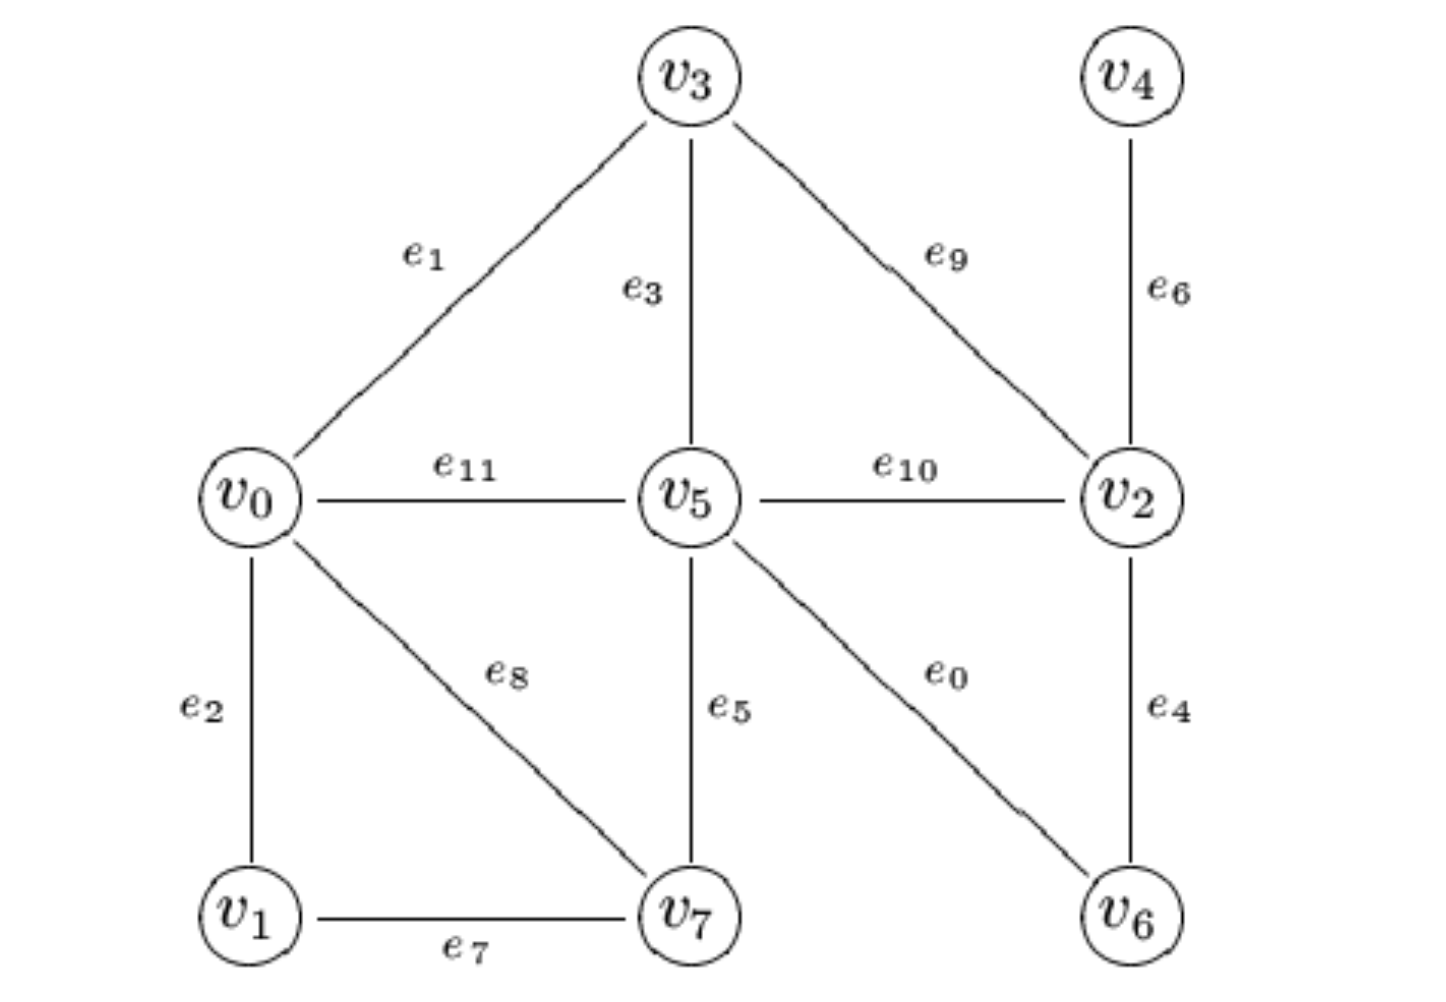
\includegraphics[width=0.4\textwidth]{9.16.png} % 插入图片
    \caption{测验题9.16用图}
\end{figure}

A. 顶点集 $E_1=\left\{e_0, e_5, e_9, e_{10}\right\}$ 是上图的一个边割集。

B. 顶点集 $E_2=\left\{e_2, e_7\right\}$ 是上图的一个边割集。

C. 顶点集 $E_3=\left\{e_1, e_5, e_{11}\right\}$ 是上图的一个边割集。

D. 上图的边连通度是2。

\textcolor{red}{答案:BC}

\subsubsection{测验题9.23}

使用广度优先策略从顶点$v_1$开始对下面的无向图进行顶点遍历,下面哪些说法是正确的?

\begin{figure}[htbp]
  \centering
  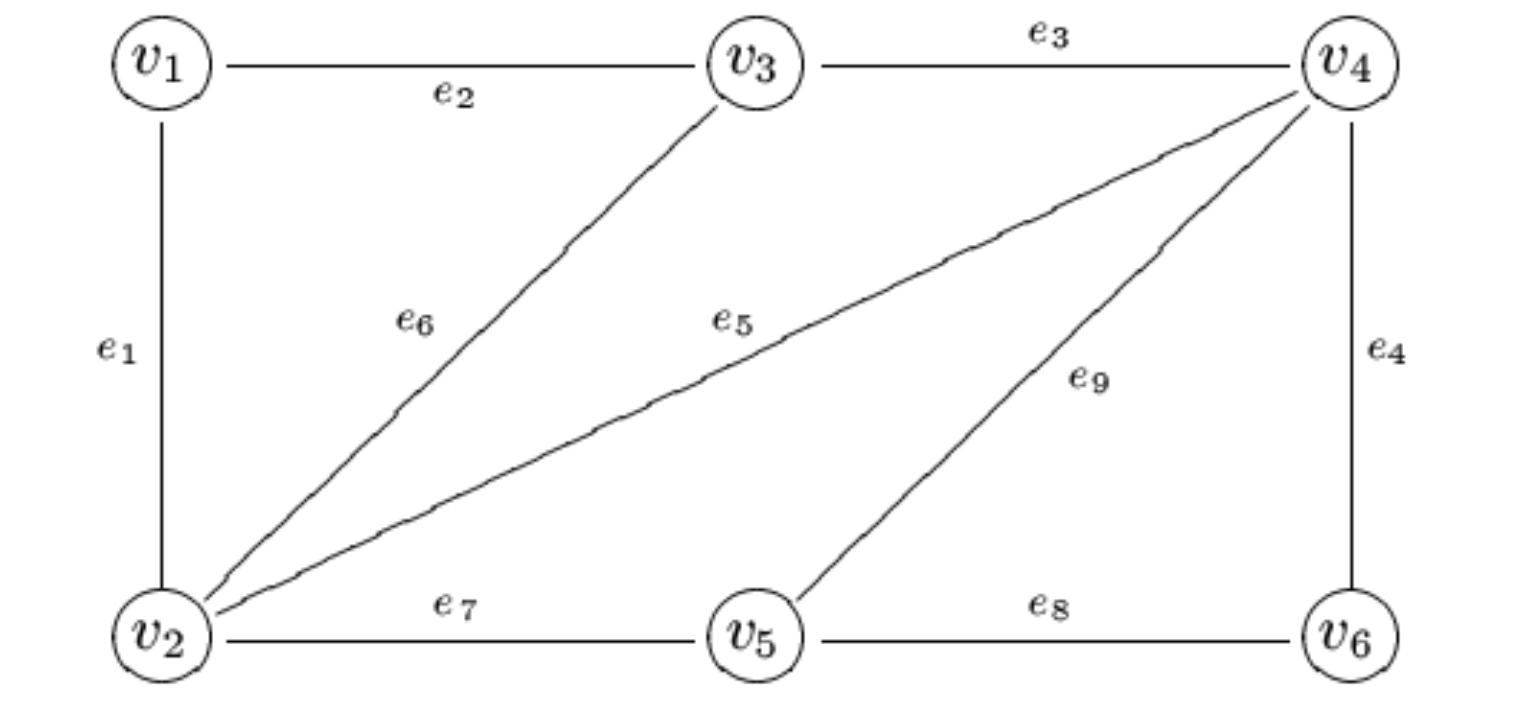
\includegraphics[width=0.4\textwidth]{9.23.png} % 插入图片
  \caption{测验题9.23用图}
\end{figure}


A. 顶点序列 $v_1 v_2 v_3 v_4 v_6 v_5$ 是一个可能的先广遍历结果。

B. 顶点序列 $v_1 v_3 v_2 v_4 v_5 v_6$ 是一个可能的先广遍历结果。

C. 顶点序列 $v_1 v_2 v_5 v_4 v_3 v_6$ 是一个可能的先广遍历结果。

D. 顶点序列 $v_1 v_2 v_3 v_5 v_4 v_6$ 是一个可能的先广遍历结果。

\textcolor{red}{答案:BD}

\subsubsection{测验题9.27}

关于无向树的基本性质,下面哪些说法是正确的?

A.无向树删除一条边之后总是得到两个连通分支。

B,无向树在任意两个不相邻顶点增加一条新边总得到唯一一个回路。

C.如果一个无向图的边数等于顶点数减1,则这个图是一棵无向树。

D,如果一个无向图的每条边都是桥,则这个图是一棵无向树。

\textcolor{red}{答案:AB}

\subsubsection{测验题9.34}

如果T是一棵满3叉树(满3元树),且有13片叶子,则它总共有(1)个顶点,其中有(2)个内部顶点。

\textcolor{red}{答案:(1) 19, (2) 6}

\subsubsection{测验题9.36}

如果T是一棵平衡满3叉树(平衡满3元树),且总共有64个顶点,则它有(1)个内部顶点和(2)片叶子,且树高为(3)。

\textcolor{red}{答案:(1) 21, (2) 43, (3) 4}

\subsubsection{测验题9.37}

如果对下面二叉树顶点实施广度优先遍历策略,则遍历结果是?

\begin{figure}[htbp]
  \centering
  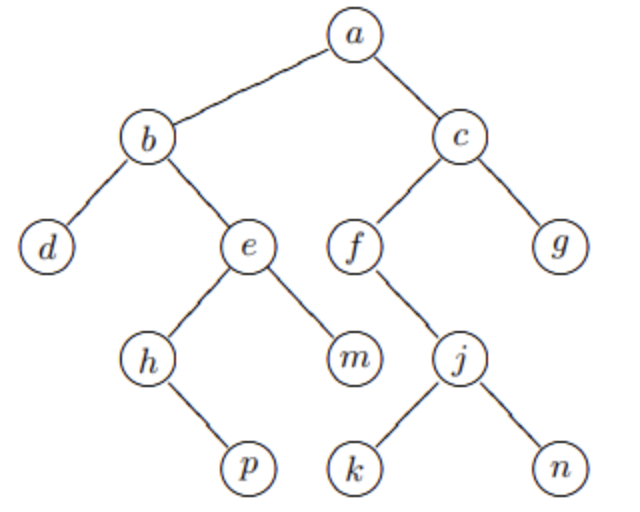
\includegraphics[width=0.35\textwidth]{9.37.png} % 插入图片
  \caption{测验题9.37用图}
\end{figure}


A. 顶点序列: $a \quad b \quad c \quad d \quad e \quad f \quad g \quad h \quad m \quad j \quad p \quad k \quad n$

B. 顶点序列: $a \quad b \quad d \quad e \quad h \quad m \quad p \quad c \quad f \quad g \quad j \quad k \quad n$

C. 顶点序列: $a \quad b \quad d \quad e \quad h \quad p \quad m \quad c \quad f \quad j \quad k \quad n \quad g$

D. 顶点序列: $a \quad b \quad d \quad h \quad p \quad e \quad m \quad f \quad k \quad j \quad n \quad c \quad g$

\textcolor{red}{答案:A}

\subsubsection{测验题9.39}

下面二叉树顶点的前序遍历结果是?

\begin{figure}[htbp]
  \centering
  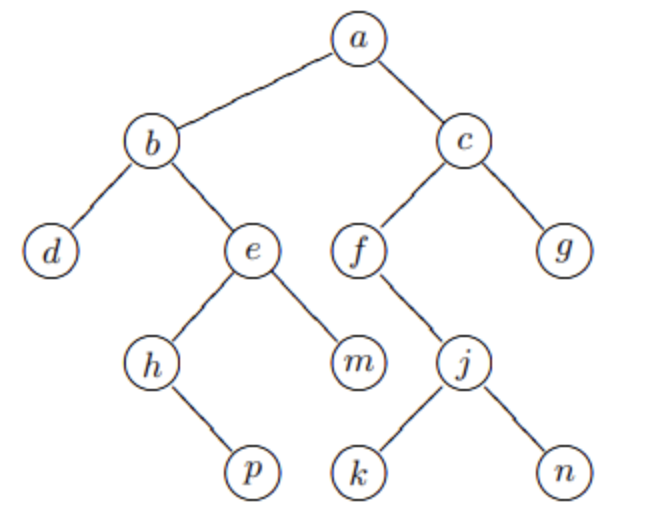
\includegraphics[width=0.35\textwidth]{9.39.png} % 插入图片
  \caption{测验题9.39用图}
\end{figure}

A. 顶点序列: $a \quad b \quad c \quad d \quad e \quad f \quad g \quad h \quad m \quad j \quad p \quad k \quad n$

B. 顶点序列: $a \quad b \quad d \quad e \quad h \quad m \quad p \quad c \quad f \quad j \quad k \quad n \quad g$

C. 顶点序列: $a \quad b \quad d \quad e \quad h \quad m \quad p \quad c \quad f \quad g \quad j \quad k \quad n$

D. 顶点序列: $a \quad b \quad d \quad h \quad p \quad e \quad m \quad f \quad k \quad j \quad n \quad c \quad g$

\textcolor{red}{答案:B}

\subsubsection{测验题9.61}

下面哪些图是极大平面图?

\begin{figure}[htbp]
    \centering
    \begin{minipage}[t]{0.35\textwidth}
        \centering
        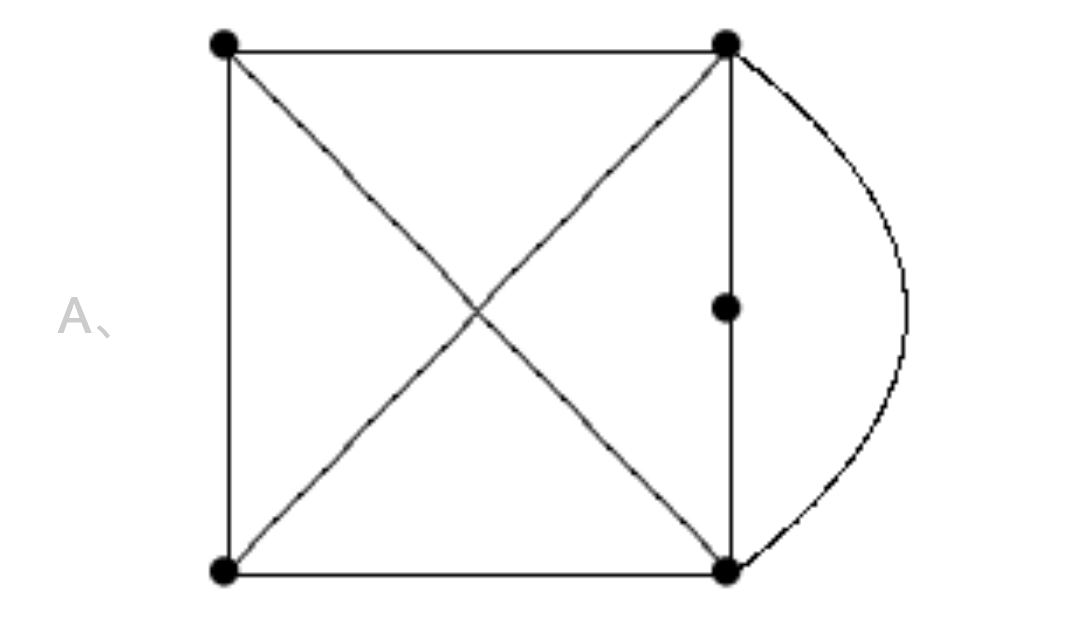
\includegraphics[width=1\textwidth]{9.61_1.png} % 插入图片
	      \vspace{-0.3cm}
        \caption{测验题9.61 A选项}
    \end{minipage}
    % \hfill
	  \hspace{0.1\textwidth} % 调整这里的值来改变两张图片之间的间距
    \begin{minipage}[t]{0.35\textwidth}
        \centering
        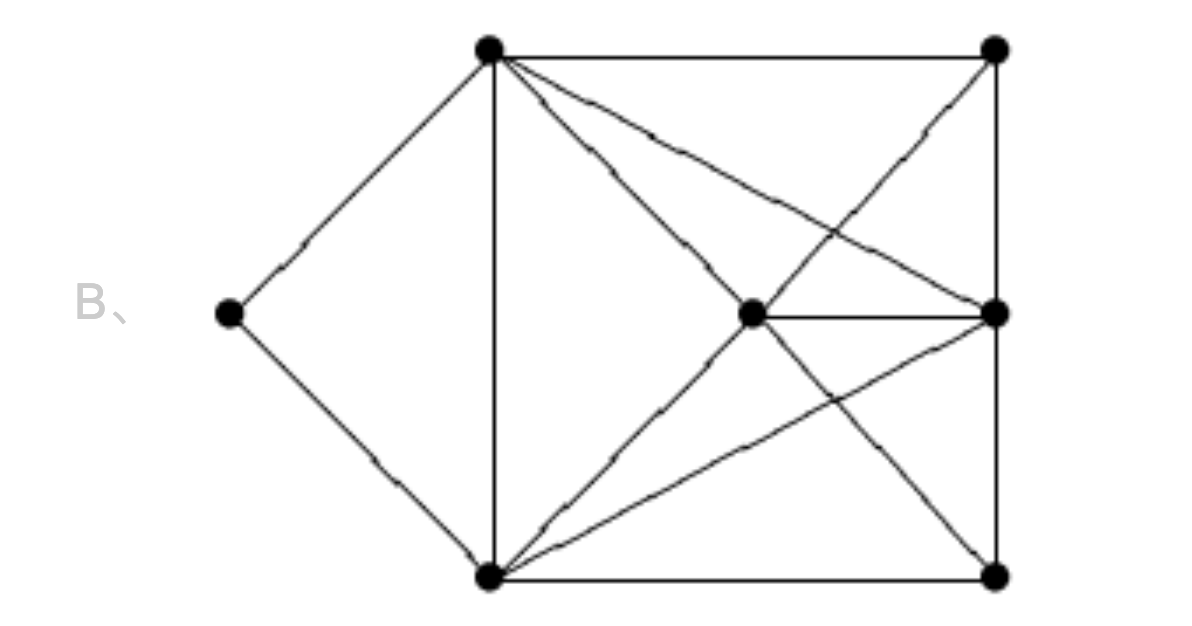
\includegraphics[width=1\textwidth]{9.61_2.png} % 插入图片
	      \vspace{-0.3cm}
        \caption{测验题9.61 B选项}
\end{minipage}
\end{figure}

\begin{figure}[htbp]
    \centering
    \begin{minipage}[t]{0.35\textwidth}
        \centering
        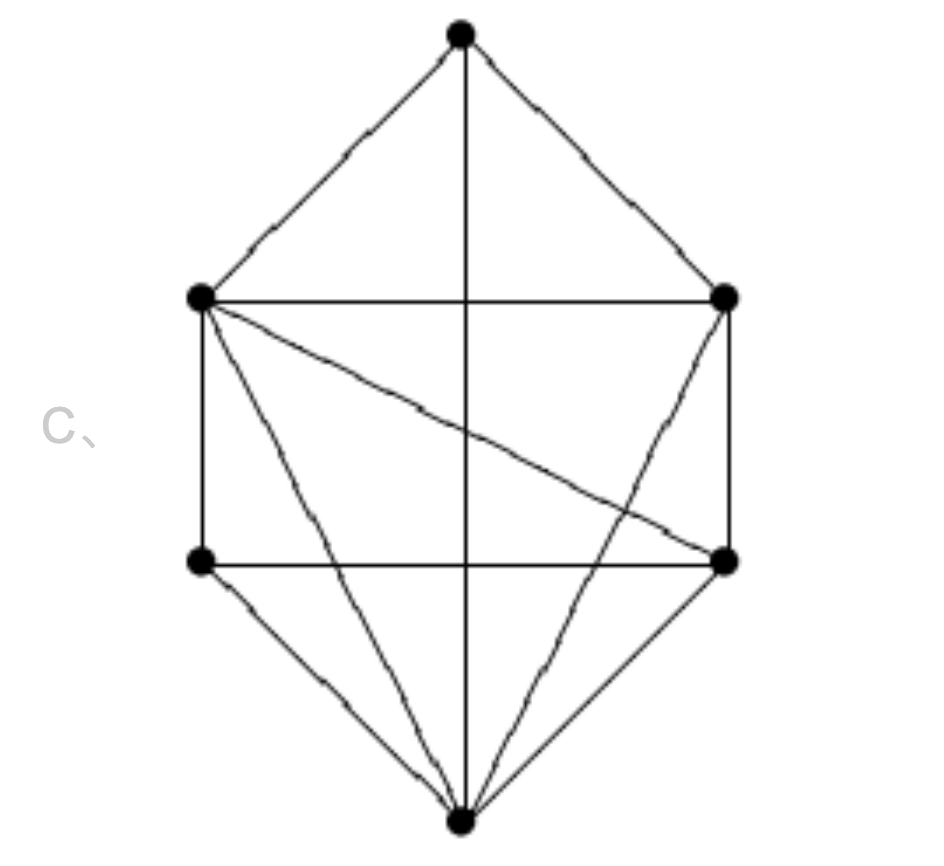
\includegraphics[width=1\textwidth]{9.61_3.png} % 插入图片
	      \vspace{-0.3cm}
        \caption{测验题9.61 C选项}
    \end{minipage}
    % \hfill
	  \hspace{0.1\textwidth} % 调整这里的值来改变两张图片之间的间距
    \begin{minipage}[t]{0.35\textwidth}
        \centering
        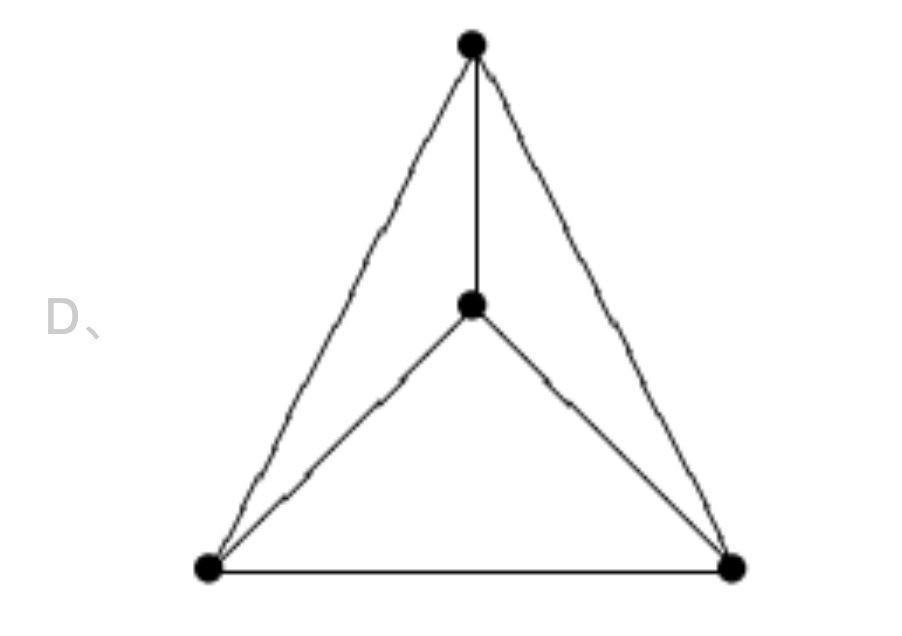
\includegraphics[width=1\textwidth]{9.61_4.png} % 插入图片
	      \vspace{-0.3cm}
        \caption{测验题9.61 D选项}
\end{minipage}
\end{figure}

\textcolor{red}{答案:CD}

\subsubsection{测验题9.64}

设平面图$G$的顶点数是$n$,边数是$m$,面数是$d$,下面哪些说法是正确的?

A. 若 $G$ 是极大平面图,则 $m=3 n-6$ 且 $d=2 n-4$ 。

B. 若 $m=3 n-6$ 且 $d=2 n-4$ ,则 $G$ 是极大平面图。

C. 对于任意平面图 $G$ ,总有 $n-m+d=2$ 。

D. 对于任意平面图 $G$ ,总有 $m \leq 3 n-6$ 且 $d \leq 2 n-4$ 。

\textcolor{red}{答案:A}

\subsubsection{测验题9.65}

设图G是连通的简单平面图,顶点数n = 6,且所有顶点的度数之和是24,则图G有(1)个面,且其中外部面的度数是(2)。

\textcolor{red}{答案:(1) 8, (2) 3}

\subsubsection{测验题9.69}

A. 完全图$K_6$

B. 圈图$C_6$

C. 轮图$W_6$

D. 完全二部图$K_{6,6}$

\textcolor{red}{答案:BD}

\subsubsection{测验题9.72}

下面哪些图是哈密顿图?

A. 完全图$K_6$

B. 圈图$C_6$

C. 轮图$W_6$

D. 完全二部图$K_{6,6}$

\textcolor{red}{答案:ABCD}

\clearpage

\section{代数系统*}


\end{document}
